\documentclass{report}
\usepackage[colorinlistoftodos,prependcaption,textsize=tiny,color=green!40,linecolor=black!50]{todonotes}
%\usepackage[table,xcdraw]{xcolor}
%%%%%%%%%%%%%%%%%%%%%%%%%%%%%%%%%%%%%%%%%%%%%%%%
% Language, Encoding and Fonts
% http://en.wikibooks.org/wiki/LaTeX/Internationalization
%%%%%%%%%%%%%%%%%%%%%%%%%%%%%%%%%%%%%%%%%%%%%%%%
% Select encoding of your inputs. Depends on
% your operating system and its default input
% encoding. Typically, you should use
%   Linux  : utf8 (most modern Linux distributions)
%            latin1 
%   Windows: ansinew
%            latin1 (works in most cases)
%   Mac    : applemac
% Notice that you can manually change the input
% encoding of your files by selecting "save as"
% an select the desired input encoding. 
\usepackage[utf8]{inputenc}
\DeclareUnicodeCharacter{0176}{\^Y}


% Make latex understand and use the typographic
% rules of the language used in the document.
\usepackage[danish,english]{babel}
% Use the palatino font
\usepackage[sc]{mathpazo}
\linespread{1.05}         % Palatino needs more leading (space between lines)
% Choose the font encoding
\usepackage[T1]{fontenc}
\usepackage{float}
%%%%%%%%%%%%%%%%%%%%%%%%%%%%%%%%%%%%%%%%%%%%%%%%
% Graphics and Tables
% http://en.wikibooks.org/wiki/LaTeX/Importing_Graphics
% http://en.wikibooks.org/wiki/LaTeX/Tables
% http://en.wikibooks.org/wiki/LaTeX/Colors
%%%%%%%%%%%%%%%%%%%%%%%%%%%%%%%%%%%%%%%%%%%%%%%%
% load a colour package
\usepackage{xcolor}
\definecolor{aaublue}{RGB}{33,26,82}% dark blue
% The standard graphics inclusion package
\usepackage{graphicx}
% Set up how figure and table captions are displayed
\usepackage{caption}
\captionsetup{%
  font=footnotesize,% set font size to footnotesize
  labelfont=bf % bold label (e.g., Figure 3.2) font
}
% Make the standard latex tables look so much better
\usepackage{array,booktabs}
% Enable the use of frames around, e.g., theorems
% The framed package is used in the example environment
\usepackage{framed}


\setlength{\parindent}{0em}
\setlength{\parskip}{1em}

%%%%%%%%%%%%%%%%%%%%%%%%%%%%%%%%%%%%%%%%%%%%%%%%
% Mathematics
% http://en.wikibooks.org/wiki/LaTeX/Mathematics
%%%%%%%%%%%%%%%%%%%%%%%%%%%%%%%%%%%%%%%%%%%%%%%%
% Defines new environments such as equation,
% align and split 
\usepackage{amsmath}
% Adds new math symbols
\usepackage{amssymb}
% Use theorems in your document
% The ntheorem package is also used for the example environment
% When using thmmarks, amsmath must be an option as well. Otherwise \eqref doesn't work anymore.
\usepackage[framed,amsmath,thmmarks]{ntheorem}

%%%%%%%%%%%%%%%%%%%%%%%%%%%%%%%%%%%%%%%%%%%%%%%%
% Page Layout
% http://en.wikibooks.org/wiki/LaTeX/Page_Layout
%%%%%%%%%%%%%%%%%%%%%%%%%%%%%%%%%%%%%%%%%%%%%%%%
% Change margins, papersize, etc of the document
\usepackage[
  inner=29mm,% left margin on an odd page
  outer=29mm,% right margin on an odd page
  bmargin=40mm,
  ]{geometry}
% Modify how \chapter, \section, etc. look
% The titlesec package is very configureable
\usepackage{titlesec}
%\titleformat{\chapter}[display]{\normalfont\huge\bfseries}{\chaptertitlename\ \thechapter}{20pt}{\Huge}
%\titleformat*{\section}{\normalfont\Large\bfseries}
%\titleformat*{\subsection}{\normalfont\large\bfseries}
%\titleformat*{\subsubsection}{\normalfont\normalsize\bfseries}
\usepackage[T1]{fontenc}
\usepackage{titlesec, blindtext, color}
\definecolor{gray75}{gray}{0.75}
\newcommand{\hsp}{\hspace{20pt}}
\titleformat{\chapter}[hang]{\Huge\bfseries}{\thechapter\hsp\textcolor{gray75}{|}\hsp}{0pt}{\Huge\bfseries}


%\titleformat*{\paragraph}{\normalfont\normalsize\bfseries}
%\titleformat*{\subparagraph}{\normalfont\normalsize\bfseries}

% Clear empty pages between chapters
\let\origdoublepage\cleardoublepage
\newcommand{\clearemptydoublepage}{%
  \clearpage
  {\pagestyle{empty}\origdoublepage}%
}
\let\cleardoublepage\clearemptydoublepage

% Change the headers and footers
\usepackage{fancyhdr}
\pagestyle{fancy}
\fancyhf{} %delete everything
\renewcommand{\headrulewidth}{0pt} %remove the horizontal line in the header
%\fancyhead[RE]{\small\nouppercase\leftmark} %even page - chapter title
%\fancyhead[LO]{\small\nouppercase\rightmark} %uneven page - section title
\fancyfoot[C]{\thepage} %page number on all pages
% Do not stretch the content of a page. Instead,
% insert white space at the bottom of the page
\raggedbottom
% Enable arithmetics with length. Useful when
% typesetting the layout.
\usepackage{calc}

%%%%%%%%%%%%%%%%%%%%%%%%%%%%%%%%%%%%%%%%%%%%%%%%
% Bibliography
% http://en.wikibooks.org/wiki/LaTeX/Bibliography_Management
%%%%%%%%%%%%%%%%%%%%%%%%%%%%%%%%%%%%%%%%%%%%%%%%
\usepackage[sorting=none]{biblatex}
\addbibresource{AAUImport/bib/mybib.bib}

%%%%%%%%%%%%%%%%%%%%%%%%%%%%%%%%%%%%%%%%%%%%%%%%
% Misc
%%%%%%%%%%%%%%%%%%%%%%%%%%%%%%%%%%%%%%%%%%%%%%%%
% Add bibliography and index to the table of
% contents
\usepackage[nottoc]{tocbibind}
% Add the command \pageref{LastPage} which refers to the
% page number of the last page
\usepackage{lastpage}

\usepackage{tabularx}
\usepackage{rotating}
\usepackage{tikz}
% Add todo notes in the margin of the document
  
\usepackage{minted}
\colorlet{shadecolor}{gray!15}
\newcommand{\tabitem}{~~\llap{\textbullet}~~}
\usepackage{csquotes}
\usepackage{xcolor}
\usepackage[toc,page]{appendix}
\usepackage{amssymb}
\usepackage{diagbox}

%%%%%%%%%%%%%%%%%%%%%%%%%%%%%%%%%%%%%%%%%%%%%%%%
% Hyperlinks
% http://en.wikibooks.org/wiki/LaTeX/Hyperlinks
%%%%%%%%%%%%%%%%%%%%%%%%%%%%%%%%%%%%%%%%%%%%%%%%
% Enable hyperlinks and insert info into the pdf
% file. Hypperref should be loaded as one of the 
% last packages
\usepackage{hyperref}
%\usepackage[notocbib]{apacite}
\hypersetup{ 
	%pdfpagelabels=true,%
	plainpages=false,%
	pdfauthor={Author(s)},%
	pdftitle={Title},%
	pdfsubject={Subject},%
	bookmarksnumbered=true,%
	colorlinks=false,%
	citecolor=black,%
	filecolor=black,%
	linkcolor=black,% you should probably change this to black before printing
	urlcolor=black,%
	pdfstartview=FitH%
}


\usepackage{wrapfig}
\usepackage{afterpage}
\usepackage{lscape}


% Fixme notes. http://madsn.net/index.php?title=FiXme
\usepackage[footnote,draft,danish,silent,nomargin]{fixme}


\usepackage[smartEllipses]{markdown}

%--------------- FOR TIP AND AVOID BOXES --------------------
\usepackage[framemethod=default]{mdframed}

%--------------- FOR TIP BOX --------------------
\newenvironment{tip}{\begin{erBox}}{\hfill{\tiny}\end{erBox}}

\definecolor{wrongexample}{RGB}{238,41,18}

\newmdenv[skipabove=7pt,
skipbelow=7pt,
rightline=false,
leftline=true,
topline=false,
bottomline=false,
backgroundcolor=rightexample!10,
linecolor=rightexample,
innerleftmargin=5pt,
innerrightmargin=5pt,
innertopmargin=5pt,
innerbottommargin=5pt,
leftmargin=0cm,
rightmargin=0cm,
linewidth=4pt]{erBox}
%--------------- END TIP BOX --------------------


%--------------- FOR AVOID BOX --------------------
\newenvironment{avoid}{\begin{ewBox}}{\hfill{\tiny}\end{ewBox}}

\definecolor{rightexample}{RGB}{31,181,0}

\newmdenv[skipabove=7pt,
skipbelow=7pt,
rightline=false,
leftline=true,
topline=false,
bottomline=false,
backgroundcolor=wrongexample!10,
linecolor=wrongexample,
innerleftmargin=5pt,
innerrightmargin=5pt,
innertopmargin=5pt,
innerbottommargin=5pt,
leftmargin=0cm,
rightmargin=0cm,
linewidth=4pt]{ewBox}
%--------------- END AVOID BOX --------------------

\newenvironment{issuebox}{\begin{eiBox}}{\hfill{\tiny}\end{eiBox}}

\definecolor{issue}{RGB}{0,142,204}
%\definecolor{issueexample}{RGB}{31,181,0}

\newmdenv[skipabove=7pt,
skipbelow=7pt,
rightline=false,
leftline=true,
topline=false,
bottomline=false,
backgroundcolor=issue!10,
linecolor=issue,
innerleftmargin=5pt,
innerrightmargin=5pt,
innertopmargin=5pt,
innerbottommargin=5pt,
leftmargin=0cm,
rightmargin=0cm,
linewidth=4pt]{eiBox}


\newenvironment{goal}{\begin{egBox}}{\hfill{\tiny}\end{egBox}}

\definecolor{goalcolor}{rgb}{0.44, 0.16, 0.39}
%\definecolor{issueexample}{RGB}{31,181,0}


\newmdenv[skipabove=7pt,
skipbelow=7pt,
rightline=false,
leftline=true,
topline=false,
bottomline=false,
backgroundcolor=goalcolor!10,
linecolor=goalcolor,
innerleftmargin=5pt,
innerrightmargin=5pt,
innertopmargin=5pt,
innerbottommargin=5pt,
leftmargin=0cm,
rightmargin=0cm,
linewidth=4pt]{egBox}




% ¤¤ Opsaetning af listings ¤¤ %
\definecolor{commentGreen}{RGB}{34,139,24}
\definecolor{stringPurple}{RGB}{208,76,239}

% ¤¤ Misc. ¤¤ %
\usepackage{listings}						% Placer kildekode i dokumentet med \begin{lstlisting}...\end{lstlisting}

\usepackage{xcolor} 
% farver til syntax highlighting i vores sprog

\usepackage{euscript}

\definecolor{brickred}{rgb}{0.8, 0.25, 0.33}
\definecolor{brightgreen}{rgb}{0.2539, 0.793, 0.3633}
\definecolor{corn}{rgb}{0.98, 0.93, 0.36}


\newcommand\codeil{\lstinline}
\newcommand\codeilblack{\lstinline[keywordstyle={}]}

\newcommand*{\todoerror}[1]{\todo[color=brickred]{#1}}
\newcommand*{\todowarning}[1]{\todo[color=corn]{#1}}
\newcommand*{\todomessage}[1]{\todo[color=brightgreen]{#1}}


% see, e.g., http://en.wikibooks.org/wiki/LaTeX/Formatting#Hyphenation
% for more information on word hyphenation
\hyphenation{ex-am-ple hy-phen-a-tion short}
\hyphenation{long la-tex}

% see, e.g., http://en.wikibooks.org/wiki/LaTeX/Customizing_LaTeX#New_commands
% for more information on how to create macros

%%%%%%%%%%%%%%%%%%%%%%%%%%%%%%%%%%%%%%%%%%%%%%%%
% Macros for the titlepage
%%%%%%%%%%%%%%%%%%%%%%%%%%%%%%%%%%%%%%%%%%%%%%%%
%Creates the aau titlepage
\newcommand{\aautitlepage}[3]{%
  {
    %set up various length
    \ifx\titlepageleftcolumnwidth\undefined
      \newlength{\titlepageleftcolumnwidth}
      \newlength{\titlepagerightcolumnwidth}
    \fi
    \setlength{\titlepageleftcolumnwidth}{0.4\textwidth-\tabcolsep}
    \setlength{\titlepagerightcolumnwidth}{\textwidth-2\tabcolsep-\titlepageleftcolumnwidth}
    %create title page
    \thispagestyle{empty}
    \noindent%
    \begin{tabular}{@{}ll@{}}
      \parbox{\titlepageleftcolumnwidth}{
        \iflanguage{danish}{%
          \includegraphics[width=\titlepageleftcolumnwidth]{"AAUImport/figures/aau_logo_da"}
        }{%
          \includegraphics[width=125pt]{"AAUImport/figures/aau_logo_en"}
        }
      } &
      \parbox{\titlepagerightcolumnwidth}{\raggedleft\sf\small
        #2
      }\bigskip\\
       #1 &
      \parbox[t]{\titlepagerightcolumnwidth}{%
      \textbf{Abstract:}\bigskip\par
        \fbox{\parbox{\titlepagerightcolumnwidth-2\fboxsep-2\fboxrule}{%
          #3
        }}
      }\\
    \end{tabular}
    \vfill
    \iflanguage{danish}{%
      \noindent{\footnotesize\emph{Rapportens indhold er frit tilgængeligt, men offentliggørelse (med kildeangivelse) må kun ske efter aftale med forfatterne.}}
    }{%
      \noindent{\footnotesize\emph{The content of this report is freely available, but publication (with reference) may only be pursued due to agreement with the author.}}
    }
    \clearpage
  }
}

%Create english project info
\newcommand{\englishprojectinfo}[8]{%
  \parbox[t]{\titlepageleftcolumnwidth}{
    \textbf{Title:}\\ #1\bigskip\par
    \textbf{Theme:}\\ #2\bigskip\par
    \textbf{Project Period:}\\ #3\bigskip\par
    \textbf{Project Group:}\\ #4\bigskip\par
    \textbf{Participants:}\\ #5\bigskip\par
    \textbf{Supervisor:}\\ #6\bigskip\par
    %\textbf{Copies:} #7\bigskip\par
    \textbf{Page Numbers:} \pageref{LastPage}\bigskip\par
    \textbf{Date of Completion:}\\ #8
  }
}

%Create danish project info
\newcommand{\danishprojectinfo}[8]{%
  \parbox[t]{\titlepageleftcolumnwidth}{
    \textbf{Titel:}\\ #1\bigskip\par
    \textbf{Tema:}\\ #2\bigskip\par
    \textbf{Projektperiode:}\\ #3\bigskip\par
    \textbf{Projektgruppe:}\\ #4\bigskip\par
    \textbf{Deltager(e):}\\ #5\bigskip\par
    \textbf{Vejleder(e):}\\ #6\bigskip\par
    \textbf{Oplagstal:} #7\bigskip\par
    \textbf{Sidetal:} \pageref{LastPage}\bigskip\par
    \textbf{Afleveringsdato:}\\ #8
  }
}

%%%%%%%%%%%%%%%%%%%%%%%%%%%%%%%%%%%%%%%%%%%%%%%%
% An example environment
%%%%%%%%%%%%%%%%%%%%%%%%%%%%%%%%%%%%%%%%%%%%%%%%
\theoremheaderfont{\normalfont\bfseries}
\theorembodyfont{\normalfont}
\theoremstyle{break}
\def\theoremframecommand{{\color{gray!50}\vrule width 5pt \hspace{5pt}}}
\newshadedtheorem{exa}{Example}[chapter]
\newenvironment{example}[1]{%
		\begin{exa}[#1]
}{%
		\end{exa}
}

\newcounter{defcounter}
\setcounter{defcounter}{0}
\newenvironment{hypothesis}{%
\addtocounter{equation}{-1}
\refstepcounter{defcounter}
\renewcommand\theequation{H.\thedefcounter}
\begin{equation}}
{\end{equation}}

\newcounter{subcounter}
\setcounter{subcounter}{0} % Problemet er hvis man f.eks skal lave en ny subhypotese til H7, så vil den første være H.7.3 nu, for. Jo hvis det er casen, så er det no stress
%Ja, men tror du ikke det kun er hyp 5 der får subhyps?
%Ellers laver vi bare en subhypothesis2 command med en ny counter <--- trueeeee
%Nice fix *highfive*
%Nice *fistbump*
%Hvorfor fistbumper du en highfive din retard?
%Shit det var akavet, nu tør jeg ikke tage i grupperummet igen :S
%Nej du må hellere blive væk for evigt
% *græder*
%*griner*
%*grinder*? - nej
%Og så levede de lykkeligt til deres dages ende <- det her

\newenvironment{subhypothesis}{%
%\addtocounter{equation}{0}
\refstepcounter{subcounter} %denne linie incrementer subcounter, tror jeg
\renewcommand\theequation{H.5.\thesubcounter}
\begin{equation}}
{\end{equation}}

% \newcounter{snippetcounter}
% \setcounter{snippetcounter}{0}
% \newenvironment{pythonsnippet}{%
% \addtocounter{figure}{-1}
% \refstepcounter{snippetcounter}
% \renewcommand\thefigure{Code Snippet \thesnippetcounter}
% \begin{figure}[H]
% \begin{cmintedlinenos}[linenos]{python}}
% {\end{cmintedlinenos}\end{figure}}

%\usepackage{subcaption}
\usepackage{booktabs}
\usepackage[norule]{footmisc} %used to remove rule from footnotes
\usepackage{longtable} %used for the semantic rule tables
\usepackage{floatflt,amsmath,amssymb} %used to make the semantic fractions
\usepackage[ligature, inference]{semantic}
\usepackage{graphicx}
\usepackage{caption}
\usepackage{wrapfig, tikz}
\usepackage{floatflt}
%\usepackage{subfig}
\usepackage{afterpage}
\usepackage{listings}

\usepackage{morewrites}

\usepackage{xpatch,letltxmacro}
\usepackage{longtable}
\usepackage{pgfplots}
\usepackage{pdfpages}
\usepackage{lipsum}
\usepackage{pdfpages}
\usepackage{glossaries}
%\usepackage{glossaries-extra}
\usepackage{xcolor}
\usepackage{tabularx}
\usepackage[color, leftbars]{changebar}
\usepackage{multicol}
\usepackage{amssymb}
\usepackage{amsmath}
\usepackage{figsize}



\definecolor{OliveGreen}{rgb}{0,0.6,0}
\definecolor{myorange}{rgb}{1.0, 0.63, 0.48}
\definecolor{mygreen}{rgb}{0.74, 0.85, 0.34}
\definecolor{myblue}{rgb}{0, 240, 240}

\setlength\changebarsep{5pt}

\makeglossaries
\loadglsentries{glossaries.tex}

\pgfplotsset{width=10cm,compat=1.9}

\usemintedstyle{}
\newcommand\mynumberformat{\def\FancyVerbFormamtLine##1{{\theFancyVerbLine} ##1}}
\LetLtxMacro{\cmintedlinenos}{\minted}
\let\endcmintedlinenos\endminted
\xpretocmd{\cmintedlinenos}{\setminted{linenos=true}\RecustomVerbatimEnvironment{Verbatim}{BVerbatim}{formatcom=\mynumberformat}{}}{}{}

\LetLtxMacro{\cminted}{\minted}
\let\endcminted\endminted
\xpretocmd{\cminted}{\RecustomVerbatimEnvironment{Verbatim}{BVerbatim}{}}{}{}
\newcommand{\changelocaltocdepth}[1]{%
  \addtocontents{toc}{\protect\setcounter{tocdepth}{#1}}%
  \setcounter{tocdepth}{#1}%
}

\lstset{
 % basicstyle=\itshape,
  xleftmargin=3em,
  literate={->}{$\rightarrow$}{2}
           {α}{$\alpha$}{1}
           {δ}{$\delta$}{1}
           {lambda}{{$\lambda$}}{1}
}
\newcommand\Tstrut{\rule{0pt}{4ex}}         % = `top' strut
\newcommand\Bstrut{\rule[-4ex]{0pt}{0pt}}   % = `bottom' strut
\newcommand{\ldb}{\mathopen{\lbrack\!\lbrack}} 
\newcommand{\rdb}{\mathclose{\rbrack\!\rbrack}}
\newcommand\blankpage{%
    \null
    \thispagestyle{empty}%
    \addtocounter{page}{-1}%
    \newpage}

\usepackage{etoolbox}
\usepackage{hyperref}
\addto\extrasenglish{
    \def\chapterautorefname{Chapter}
    \def\sectionautorefname{Section}
    \def\subsectionautorefname{Section}
    \def\subsubsectionautorefname{Section}
    \def\tableautorefname{Table}
    \def\figureautorefname{Figure}
}
\makeatletter
\pretocmd{\part}{\addtocontents{toc}{\protect\addvspace{-8\p@}}}{}{}
\pretocmd{\chapter}{\addtocontents{toc}{\protect\addvspace{-5\p@}}}{}{}
\pretocmd{\section}{\addtocontents{toc}{\protect\addvspace{-6\p@}}}{}{}
\pretocmd{\subsection}{\addtocontents{toc}{\protect\addvspace{-7\p@}}}{}{}
\makeatother

\usepackage{listings}
\usepackage{xcolor}

\definecolor{codegreen}{rgb}{0,0.6,0}
\definecolor{codegray}{rgb}{0.5,0.5,0.5}
\definecolor{codepurple}{rgb}{0.58,0,0.82}
\definecolor{backcolour}{rgb}{0.95,0.95,0.92}

\lstdefinestyle{mystyle}{
    commentstyle=\color{codegreen},
    keywordstyle=\color{magenta},
    numberstyle=\tiny\color{codegray},
    stringstyle=\color{codepurple},
    basicstyle=\ttfamily\footnotesize,
    breakatwhitespace=false,         
    breaklines=true,                 
    captionpos=b,                    
    keepspaces=true,                 
    numbers=left,                    
    numbersep=5pt,                  
    showspaces=false,                
    showstringspaces=false,
    showtabs=false,                  
    tabsize=2
}

\lstset{style=mystyle}

\begin{document}
\pagestyle{empty} %disable headers and footers
\pagenumbering{roman} %use roman page numbering in the frontmatter

%\includepdf[width=1.38\textwidth, pages=-]{Report/WORST.pdf}
\pdfbookmark[0]{Front page}{label:frontpage}%
\begin{titlepage}
  \addtolength{\hoffset}{0.5\evensidemargin-0.5\oddsidemargin} %set equal margins on the frontpage - remove this line if you want default margins
  \noindent%
  \begin{tabular}{@{}p{\textwidth}@{}}
    \toprule[2pt]
    \midrule
    \vspace{0.2cm}
    \begin{center}
    \Huge{\textbf{
      8th Semester Project Title% insert your title here
    }}
    \end{center}
    \begin{center}
      \Large{     
      Subtitle% insert your subtitle here
      }
    \end{center}
    \vspace{0.2cm}\\
    \midrule
    \toprule[2pt]
  \end{tabular}
  \begin{center}
  
    \vspace{12cm}
    {\large
      Project Report%Insert document type (e.g., Project Report)
    }\\
    %\vspace{0cm}
    {\Large
      SW  E21%Insert your group name or real names here
    }

  \end{center}
  \vfill
  \begin{center}
  Aalborg University\\
  Department of Computer Science
  \end{center}
\end{titlepage}
\clearpage
%
\newpage
\pdfbookmark[0]{English title page}{label:titlepage_en}
\aautitlepage{%
  \englishprojectinfo{
    \textit{Indoor Position Estimation in Multi-Level Buildings}%title
  }{%
    8th Semester Project (Mobility) %theme
  }{%
    Spring Semester 2021 %project period
  }{%
    SW807F21
  }{%
    %list of group members
    Abiram Mohanaraj, \\
    Cecilie Hyrup Madsen,\\
    Elisabeth Niemeyer Laursen, \\
    Martin Pekár Christensen, \\
    Melanie Selman,\\
    Mikkel Filip Jensen\\
  }{%
    %list of supervisors
    Dalin Zhang
  }{%
    1 % number of printed copies
  }{%
    27th of May, 2021 % date of completion
  }%
}{%department and address
  \textbf{Department of Computer Science}\\
  Aalborg University\\
  \href{http://www.aau.dk}{http://www.aau.dk}
}{
%\todo{Husk ikke at bruge passive voice. Derudover er projektet ikke basered rundt om Kaggle. Vi bruger bare deres dataset.}
In this project, we investigate the task of indoor positioning in multi-level buildings. This can be a complex task as there currently are no optimal solutions. Therefore, the goal of this project is to predict indoor positions based on real-time sensor data from smartphones. 
To meet this goal, we conduct several experiments to find the most accurate solution. We also propose three hybrid architectures, which incorporates Pedestrian Dead Reckoning (PDR) and Location Fingerprinting (LFP). Our experiments consist of multiple algorithms within LFP and IMU based methods, and lastly our proposed hybrid methods. To evaluate these methods, we use a dataset provided by the Indoor Navigation \& Location competition at Kaggle, which consists of a variety of sensor data from smartphones and location data.
\\

We also evaluate the positioning methods by comparing the Mean Position Error (MPE). We also conclude that a hybrid approach, combining the IMU method Pedestrian Dead Reckoning (PDR) as primary with Gradient Boosting Decision Tree (GBDT) as support yields the best performance with a Mean Position Error (MPE) of 18.59. GBDT was chosen since it performed best with a MPE of 23.21. The performance of our best hybrid solution performed 19.91\% better compared to GBDT.
}
%\cleardoublepagehttps://www.overleaf.com/project/5f51e9d829099c000199193c
%\afterpage{\blankpage}%
%\newpage
%Insert Preface text

\section*{Reading Guide}
%
%% MOTIVATION
\todo{Mangler kilde(r).}
There are many reasons why indoor positioning is worth exploring. Since \gls{gps} are not accurate enough in terms of indoor navigation, the indoor positioning can be used for several different occasions, for instance indoor navigation, location-based notifications, and optimisation of work efficiency.

Indoor navigation could be used for helping the user navigate through office buildings, airports, hospitals etc. This could help users save time and give them a better experience. When the location of the user is known, it is also possible to send them messages based on their location in the airport, store etc. For instance, you could send them a message about an offer on a product when you can see that they are in the duty-free shop in the airport. 

By using indoor location, you could also gain insight into the movement behaviour of people in a certain place. With this information, you could for instance see if your staff always takes the shortest path, or if there are areas of your store that people do not visit. With this information, we could create a more intuitive architecture of our buildings.\cite{IPSMapsPeople}
%https://blog.mapspeople.com/mapsindoors/indoor-positioning-101
%\newpage

\cleardoublepage
\pdfbookmark[0]{Contents}{label:contents}
\pagestyle{fancy} %enable headers and footers again
\pagenumbering{roman}

\setcounter{tocdepth}{1}
\tableofcontents
%\afterpage{\blankpage}

\newpage\pagenumbering{arabic}


\chapter{Data Standard}
\section{Feature Engineering}\label{sec:feature_eng}
In this section, we will elaborate on the feature engineering for the experiments. Feature engineering concerns extracting useful features from the dataset.  %The idea behind data pipeline is to automate the workflow for training and testing a model. A data pipeline consists of a sequence of data processing components, where the output of one component would be the input to another. For the position estimation in this project, we need a data pipeline to model the different scene analysis algorithms and evaluate them as well as the \gls{imu}-based algorithms. The responsibility of the data pipeline to process the data from the preprocessing step to a format directly usable by the different algorithms.
For the position estimation in this project, we need a feature engineering component to model the raw training data for the different location fingerprinting algorithms and evaluate them, as well as the \gls{imu}-based algorithms. This is necessary as the raw training data is not directly usable for the location fingerprinting algorithms. %The responsibility of the data pipeline to process the data from the preprocessing step to a format directly usable by the different algorithms.

During the training and evaluation of the algorithms and models, we will only be considering the data from the sites in the test dataset provided by the competition. This limitation is imposed due to time constraints and the increased complexity. We expect that these chosen sites are representative of them all. Considering that we will be creating separate models for each site, this is a reasonable approach to sample the dataset. The sites in question are 24 out of 204 sites in the training dataset.

The formats usable by the estimation algorithms can roughly be classified into three types. The first type is an \gls{rssi} dataset, which is a dataset of feature samples and ground truth for the samples. In another type, the data format is used by algorithms specialised for time series data. A third type of data format is for the \gls{imu}-based methods. The last type of data format is for the hybrid. Implementation-wise, this is a combination of the features engineering for the \gls{rssi} and \gls{imu} data. The output format for the hybrid feature engineering should be a map for each path from timestamp to the features.
%In this format, the ordering of the feature samples and ground truth data does not matter, and this format is also mainly used by most of the location fingerprinting algorithms discussed in \textbf{\autoref{sec:scene_analysis}}. 
%In another type, the data format is used by algorithms specialised for time series data. This means that the feature samples should be organised into series, where each series contains a sequence of feature samples. These series should be organised into an list-based structure, and the corresponding ground truth data should be stored into another list-based structure, where \textit{i}th entry in feature series corresponds to the \textit{i}th entry in the ground truth series. 
%The last type of data format is for the \gls{imu}-based methods. The purpose of the formatting of the data for the \gls{imu}-based methods is purely for evaluating the methods as no optimization of a model is necessary for this type of indoor position estimation.

%The features will be generated separately for each site in the dataset. This implies that the models trained and algorithms used will be specific for each site.

% \begin{enumerate}
%     \item One type of data pipeline is necessary for the \gls{imu}-based algorithms as this type of algorithm requires information regarding \gls{imu} sensor and a starting GPS location.
%     \item Another type of data pipeline is necessary for the some of the scene analysis methods. Here, radio frequence data like Wi-Fi or Bluetooth is necessary as features for the algorithms. Furthermore, to train the models used by the different algorithms the actual positions for each feature is necessary. 
%     \item A third type of data pipeline concerns with processing the data for scene analysis algorithm which makes use of time series data. This means that after constructing the features from the dataset with the radio frequence data, the data should also be ordered according to the timestamp.
% \end{enumerate}
\subsection{RSSI Dataset Creation} \todo{RETTELSER HER. Beskriv intuition bag algoritmen fremfor uddybende tekst}
In \gls{rssi}-labeled dataset, the ordering of the feature samples and ground truth data does not matter, and this format is also mainly used by most of the location fingerprinting algorithms discussed in \textbf{\autoref{sec:scene_analysis}}.
The overall feature engineering data flow for the \gls{rssi}-dataset is shown in \textbf{\autoref{fig:feat_labeled}}, while the algorithm is shown in \textbf{\autoref{alg:rssi}}. The dataset outputted by the Data Preprocessing step is organised into text files where each line in the file corresponds to a sensor measurement. This is shown by the top-most box in \textbf{\autoref{fig:feat_labeled}}.

\begin{figure}[H]
    \centering
    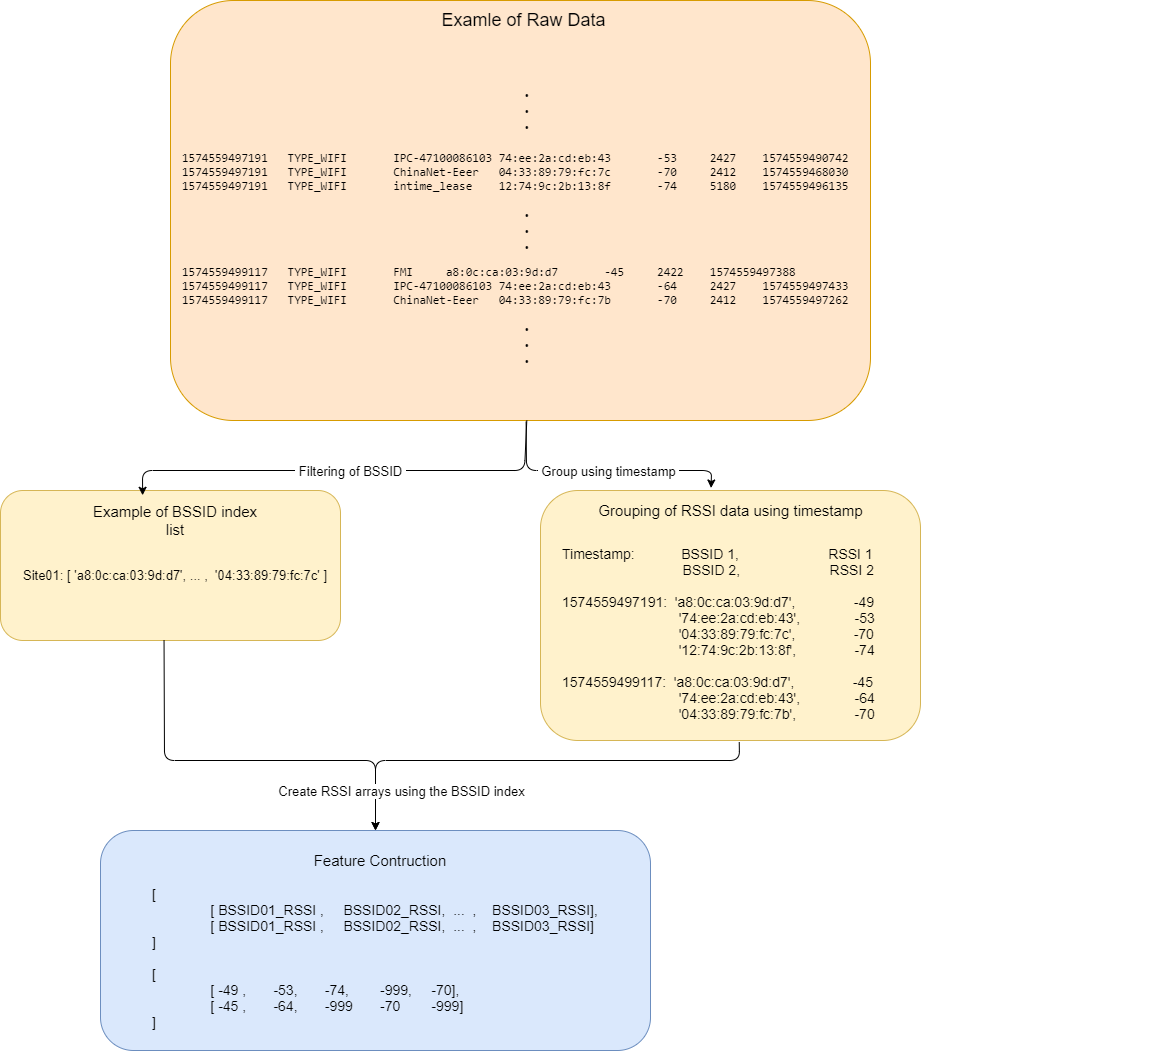
\includegraphics[width=1\textwidth]{Images/DataStandard/feat_eng_labeled (1).png}
    \caption{Labeled Dataset construction. The orange box shows a snippet of the raw dataset. }
    \label{fig:feat_labeled}
\end{figure}

As shown in \textbf{\autoref{alg:rssi}}, the feature engineering algorithm consists of a for-loop that will iterate all sites in the training data. This for-loop consists of two other for-loops, where the first will iterate through all the paths in a given site, and retrieve the relevant information. %It will hereafter append all the Wi-Fi measurements to a list, and all the waypoints to another list. 
The relevant information (\textit{wifi\_list}) will be grouped according to its timestamps, and these groups will be iterated through in the next for-loop on line 15, where the waypoint with the least difference between the group and each waypoint in the \textit{waypoints} list will be saved as the \textit{ground} result, which will be appended to the \textit{ground\_truth} list. The \gls{rssi} values from the group will be re-indexed and saved in \textit{feat}, which will be appended to the \textit{train\_data} list. As seen on line 21, the yield statement is used instead of a return statement. The yield statement indicates that we are working with a generator function. When working with a return statement, the statement would terminate the function entirely, whereas the yield statement will pause the function and save all of the states before continuing to successive calls.

\begin{algorithm}[H]
\SetAlgoLined
\SetKw{KwIn}{in}
\SetKwInOut{Input}{Input}
\Input{$\text{train\_data}$ which is organised into sites and further into paths}
\KwResult{($\text{site}_{x}$, $\text{train\_data}_{x}$, $\text{ground\_truth}_{x}$)}
 \For{$\text{site}_{x}$ \KwIn $\text{train\_data}$}{
  $\text{train\_data}_{x}$ = [], $\text{ground\_truth}_{x}$=[]\;
  Create $bssid\_index$ which is the set of BSSID values in the data for $\text{site}_{x}$\;
  \For{$\text{path}_{x}$ \KwIn $\text{site}_{x}$}{
    $wifi\_list$ = [], $waypoints$=[]\;
    \For{$measurement$ \KwIn $\text{path}_{x}$}{
        \If{$measurement$["type"]== $\text{TYPE\_WIFI}$}{
            $wifi\_list$.append($measurement$)\;
        }\ElseIf{$measurement$["type"]== $\text{waypoint}$}{
            $waypoints$.append($measurement$)
        }
    }
    Group $wifi\_list$ according to the timestamp into $grouped\_measmts$\;
    \For{$group$ \KwIn $grouped\_measmts$}{
        Calculate waypoint with least difference in timestamps between the $group$ and each waypoint in $waypoints$ and save the result as $ground$\;
        Take the RSSI-values from $group$ and reindex according to $bssid\_index$ and save in $feat$\;
        $\text{train\_data}_{x}$.append($feat$),$\text{ground\_truth}_{x}$.append($ground$)\;
    }
  }
  yield $\text{site}_{x}$,$\text{train\_data}_{x}$, $\text{ground\_truth}_{x}$\;
 }
 \caption{\gls{rssi}-labeling.}
 \label{alg:rssi}
\end{algorithm}

To create the features consisting of \gls{rssi} values, it is necessary to ensure that \gls{rssi} values are ordered such that the \textit{i}th value in a specific feature sample corresponds to data collected from one device (\gls{bssid}). This step is encapsulated by line 3 in \textbf{\autoref{alg:rssi}}. To this end, we use the \gls{bssid} values to uniquely distinguish the \gls{rssi} values from each other. Therefore, a pass over all data for a particular site is first made, where the \gls{bssid} values are collected to be used in the Feature Construction step in \textbf{\autoref{fig:feat_labeled}}. The \gls{bssid} values with less than a specific amount are then removed. This specific amount is set to 1000, but can be changed. The idea behind this filtering is that \gls{rssi} values with few occurrences will likely not contribute to the training of the models and might make it harder for the models to generalise. By performing this filtering, we observed that for approximately 5 \% of the features, all \gls{rssi} values were removed. To combat this, we include \gls{rssi} values from the test data when filtering. For the missing or unknown \gls{rssi} values, it will be set to -999 in the resulting feature. The result of collecting and filtering the \gls{bssid} values is shown \textit{Example of BSSID index} in \textbf{\autoref{fig:feat_labeled}}. 
The resulting \gls{bssid} set will be used as an index for the features. %To construct the features, a second pass over the data is made, where the measurement data is grouped by the timestamp. For each group, the \gls{rssi} values are extracted and an array is created by using the \gls{bssid} list and the \gls{rssi} values. For the \gls{bssid} indices with \gls{rssi} value in the group, the value will be set to -999.%The intuition behind this is to include a logarithmic activation function or a similar function to the input layer such that the values with -999 will have a small value. 

To gather multiple \gls{rssi} sensor measurements, we use the timestamp property in the measurements to group them together. This phase occurs in the right yellow box in \textbf{\autoref{fig:feat_labeled}}, and lines 14 to 19 in \textbf{\autoref{alg:rssi}}. The goal of location fingerprinting is to estimate the location given measurements at a certain time, making it reasonable to group with the timestamp. We will be using \gls{rssi} data, and this means that Wi-Fi and Bluetooth data can be used. As the Wi-Fi data is more prevalent in the dataset, we will be starting with this data. 
%After grouping the measurement data by the timestamp for each group, the \gls{rssi} values are extracted, and an feature sample is created by using a \gls{bssid} index for a site. For the \gls{bssid} indices without a \gls{rssi} value in the group, the value will be set to -999. To find the ground truth for each group, the temporally nearest waypoint to the group is found and treated as the ground truth along with the floor number which is specified in the file path to the data.

% \begin{wrapfigure}{r}{0.5\textwidth}
%   \begin{center}
%     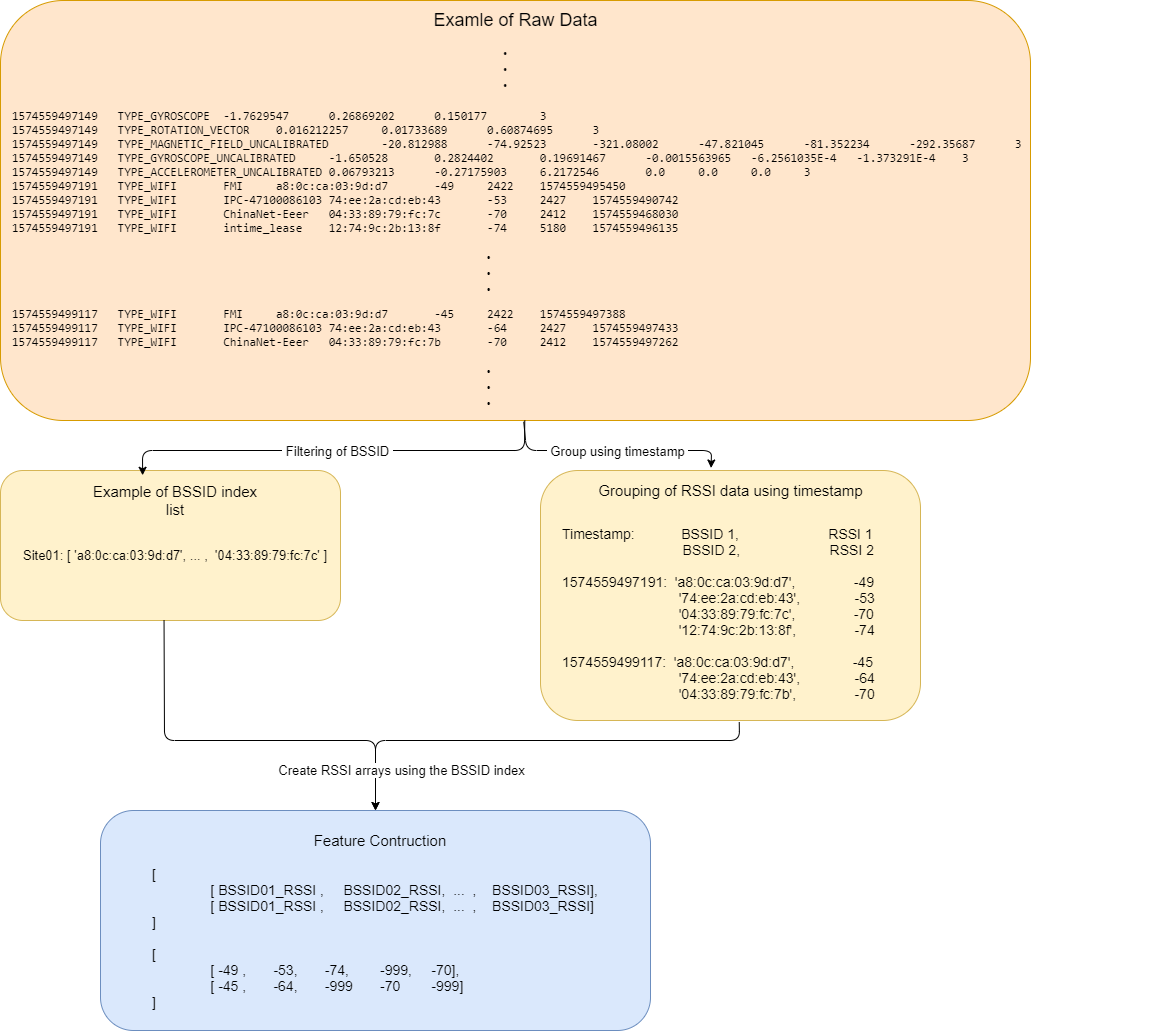
\includegraphics[width=0.48\textwidth]{Images/DataStandard/feat_eng_labeled.png}
%   \end{center}
%   \caption{Labeled Dataset Constuction}
% \end{wrapfigure}

\subsection{Time Series Data Formatting}

The time series dataset is similar to the RSSI-dataset other than the fact that the ordering of the measurements matter. 

Time-series data refers to a set of observations recorded over a given period of time at equally spaced time intervals. Time-series data is a type of sequence data, but in a time-series dataset, the observations are recorded based on timestamps. For instance, in a DNA sequence the order is important, but it is not ordered based on a timestamp \cite{Yalcın2021}. Time-series data gives us the opportunity to track changes over time, and in our case, the measurements given in the Kaggle dataset gives us the ability to track the movement of a device. 

This means that the feature samples should be organised into series, where each series contains a sequence of feature samples. These series should be organised into an list-based structure, and the corresponding ground truth data should be stored into another list-based structure, where \textit{i}th entry in feature series corresponds to the \textit{i}th entry in the ground truth series.

The algorithm for the time series labeling is very similar to the one presented in \textbf{\autoref{alg:rssi}}. The difference lies in line 5 and 21 in \textbf{\autoref{alg:time_series}}, where two new arrays are being created to hold the time series data, and afterwards appended to the training data and the ground truth data.

\begin{algorithm}[H]
\SetAlgoLined
\SetKw{KwIn}{in}
\SetKwInOut{Input}{Input}
\Input{$\text{train\_data}$ which is organised into sites and further into paths}
\KwResult{($\text{site}_{x}$, $\text{train\_data}_{x}$, $\text{ground\_truth}_{x}$)}

 \For{$\text{site}_{x}$ \KwIn $\text{train\_data}$}{
  $\text{train\_data}_{x}$ = [], $\text{ground\_truth}_{x}$=[]\;
  Create $bssid\_index$ which is the set of BSSID values in the data for $\text{site}_{x}$\;
  \For{$\text{path}_{x}$ \KwIn $\text{site}_{x}$}{
    $time\_series$ = [], $ts\_ground$=[]\;
    $wifi\_list$ = [], $waypoints$=[]\;
    \For{$measurement$ \KwIn $\text{path}_{x}$}{
        \If{$measurement$["type"]== $\text{TYPE\_WIFI}$}{
            $wifi\_list$.append($measurement$)\;
        }\ElseIf{$measurement$["type"]== $\text{waypoint}$}{
            $waypoints$.append($measurement$)
        }
    }
    Group $wifi\_list$ according to the timestamp into $grouped\_measmts$\;
    \For{$group$ \KwIn $grouped\_measmts$}{
        Calculate waypoint with least difference in timestamps between the $group$ and each waypoint in $waypoints$ and save the result as $ground$\;
        Take the RSSI-values from $group$ and reindex according to $bssid\_index$ and save in $feat$\;
        $time_series$.append($feat$),$ts_ground$.append($ground$)\;
    }
    $\text{train\_data}_{x}$.append($time\_series$),  $\text{ground\_truth}_{x}$.append($ts\_ground$)
  }
  yield $\text{site}_{x}$,$\text{train\_data}_{x}$, $\text{ground\_truth}_{x}$\;
 }
 \caption{Time Series labeling.}
 \label{alg:time_series}
\end{algorithm}
%https://online.stat.psu.edu/stat510/lesson/1/1.1



\subsection{Inertial Measurement Unit Dataset Creation}
The \gls{imu} dataset creation is for the \gls{imu}-based methods. The purpose of the formatting of the data for the \gls{imu}-based methods is purely for evaluating the methods as no learning is necessary for this type of indoor position estimation.
The basic idea with the feature engineering for the \gls{imu}-based methods is similar to the \gls{rssi}-based feature enginnering in that we once more group the \gls{imu} data according to timestamp. After the grouping, we will extract the relevant information into a list, which can then included as features.

\begin{algorithm}[H]
\SetAlgoLined
\SetKw{KwIn}{in}
\SetKwInOut{Input}{Input}
\Input{$\text{train\_data}$ which is organised into sites and further into paths}
\KwResult{($\text{path}_{x}$, $\text{train\_data}_{x}$, $\text{ground\_truth}_{x}$)}
 \For{$\text{site}_{x}$ \KwIn $\text{train\_data}$}{
  $\text{train\_data}_{x}$ = [], $\text{ground\_truth}_{x}$=[]\;
  \For{$\text{path}_{x}$ \KwIn $\text{site}_{x}$}{
    $imu\_list$ = [], $waypoints$=[]\;
    \For{$measurement$ \KwIn $\text{path}_{x}$}{
        \If{$measurement$["type"]== $\text{TYPE\_ACCELEROMETER}$}{
            $imu\_list$.append($measurement$)\;
        }\ElseIf{$measurement$["type"]== $\text{TYPE\_MAGNETIC\_FIELD}$}{
            $imu\_list$.append($measurement$)\;
        }\ElseIf{$measurement$["type"]== $\text{TYPE\_GYROSCOPE}$}{
            $imu\_list$.append($measurement$)\;
        }\ElseIf{$measurement$["type"]== $\text{waypoint}$}{
            $waypoints$.append($measurement$)
        }
    }
    Group $imu\_list$ according to the timestamp into $grouped\_measmts$\;
    \For{$group$ \KwIn $grouped\_measmts$}{
        Calculate waypoint with least difference in timestamps between the $group$ and each waypoint in $waypoints$ and save the result as $ground$\;
        $\text{train\_data}_{x}$.append($feat$),$\text{ground\_truth}_{x}$.append($ground$)\;
    }
  yield $\text{site}_{x}$,$\text{train\_data}_{x}$, $\text{ground\_truth}_{x}$\;  
  }
 }
 \caption{\gls{imu}-labeling.}
 \label{alg:imu}
\end{algorithm}


\subsection{Min-Max Normalisation} \label{sec:minmaxnormalisation}
Min-max normalisation scales features so that all features are equally significant. Although, the one disadvantage is that it handles feature outliers poorly.
Min-max normalisation is a data normalisation method described by \textbf{\autoref{eq:min_max_normalisation}}. Functions $min_A$ and $max_A$ compute the minimum and maximum value of an attribute, $A$, respectively. Given a value $v_i$ of an attribute $A$ as input, min-max normalisation computes value $v_{i}'$ in the range $[new\_min_A, new\_max_A]$.\cite{Han_Kamber_2012}

\begin{equation}
    v_{i}' = \frac{v_i - min_A}{max_A - min_A} (new\_max_A - new\_min_A) + new\_min_A
    \label{eq:min_max_normalisation}
\end{equation}

\chapter{Indoor Position Methods Theory}
\section{Pedestrian Dead Reckoning (PDR)} \label{sec:pdr}

\gls{pdr} is a positioning method, where the traveled distance and a heading are added to the known starting position \cite{pdr_smartphonebased}. The \gls{pdr} method is described in \cite{HybridPositioningPaper} and uses the \gls{imu} for positioning. The tracking of the pedestrian can be accomplished through performing step detection, step length estimations and heading estimation. Tracking a pedestrian is done in iterations, where computing a position is based on the previous position computed.

As seen in many papers, such as in \cite{pdr_smartphonebased, HybridPositioningPaper, 6987239, 6782540}, \gls{pdr} is a common solution for position estimation, and we have therefore chosen to experiment with this method. Our method is constructed with inspiration from multiple works. A graphical presentation of the method is shown in \textbf{\autoref{fig:pdr}}. The Z-axis dispersion and step detection is acquired from \cite{peakdetection}, and the step length estimation is from \cite{HybridPositioningPaper}. For the heading estimation, the toolkit \gls{ahrs} is used, where different filters from the toolkit have been researched. The different components of the method will be elaborated further on in the following sections. Each of the components have a dedicated number from 1 to 5 to make the process easier to explain. 
\\

\begin{figure}[H]
    \centering
    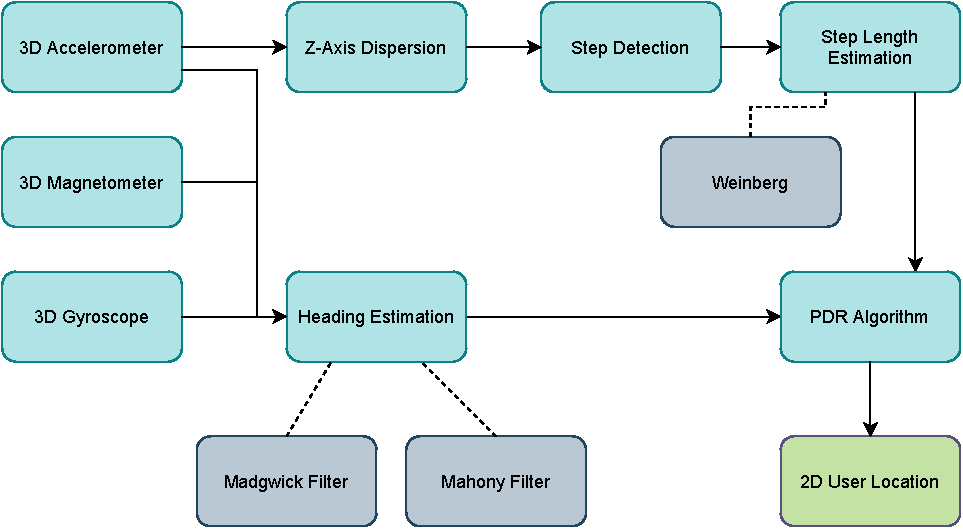
\includegraphics[scale=0.7]{Images/Experiments/pdr.pdf}
    \caption{PDR implementation architecture.}
     \label{fig:pdr}
\end{figure}

% Tag elementer fra filen geometry_based.tex fra 1.Problem_analysis til forklaring af PDR.

\subsection{Step Detection}

The general idea of step detection of a pedestrian with a smartphone is by measuring the accelerometer sensor and observe the increases and decreases in the acceleration pattern\cite{HybridPositioningPaper}. We have chosen to follow the algorithm proposed in \cite{peakdetection}. This is due to the fact that it is the only solution implementable for smartphones in a walking scenario.

The algorithm is based on the principle of dispersion, which is the extent to which a distribution is stretched or squeezed \cite{dispersion}. As seen in figure \textbf{\autoref{fig:pdr}}, the Z-axis dispersion is computed before the step detection. This step includes smoothening of the data to remove noise. This is included in the first step in \textbf{\autoref{fig:pdr}}, which is denoted by the number \textbf{1}.

For the step detection, which is \textbf{step 2} in \textbf{\autoref{fig:pdr}}, the algorithm will return a signal value if a new datapoint is a specific amount of deviations away from a moving mean. This amount of deviations is also called the z-score. The algorithm creates a separate moving mean and deviation, and signals can therefore not corrupt the threshold. The algorithm takes 3 inputs: \textit{lag}, \textit{threshold} and \textit{influence}. \textit{Lag} determines how much the input data is to be smoothened. Therefore, low lag values result in the algorithm being quicker at adapting to the input data. Since the input data for step detection vary a lot, the lag value will be low. The \textit{threshold} is the z-score at which the algorithm will return a signal. Lastly, the \textit{influence} is the impact of new signals on the mean and deviation. The influence can be between 0 and 1. If 0 is chosen as the influence, signals would be completely ignored for recalculation of a new threshold. This choice would assume stationarity, meaning that the statistical properties of a process, such as the mean, variance and the structure of the autocorrelation, do not change over time\cite{stationarity}. In our case, we are working with data from walking people in a shopping mall. Since random walking is not a stationary process, we will use a nonzero value\cite{peakdetection}. The \textit{threshold} value is set to 10, since this is the value we deemed as giving the best result for detecting steps for our data set by trial-and-error. The \textit{threshold} value is found by using a subset of the data provided by Indoor Location \& Navigation Competition from Kaggle that corresponds to a single step to evaluate when the algorithm signals a step. The \textit{lag} value is set to 2, and is found in the same way as the \textit{threshold} value.

\subsection{Step Length Estimation}

For step length estimation, there exists two methods: static and dynamic. The static method assumes a person is walking at a constant velocity, whereas the dynamic method makes use of an accelerator for dynamic estimation. Weinberg is one method for dynamic step length estimation. We have decided to use the Weinberg method due to its low error compared to other methods \cite{HybridPositioningPaper}. This is executed in \textbf{step 3} in \textbf{\autoref{fig:pdr}}.  

The Weinberg method is defined in \textbf{\autoref{eq:weinberg}}\cite{weinberg}.

\begin{equation} \label{eq:weinberg}
    l = k \sqrt[4]{a_{LPF, peak} - a_{LPF, valley}}
\end{equation}

In \textbf{\autoref{eq:weinberg}}, $k$ is a constant factor for unit conversion, $a_{LPF, peak}$ is the maximum acceleration in the z-axis and $a_{LPF, valley}$ is the minimum acceleration in the z-axis. The value $k = 0.5$ is used in \cite{HybridPositioningPaper}, and we also found that this value yielded the best result by error-and-trial.

\subsection{Heading Estimation}
\textbf{Step 4} is the heading estimation. The heading estimation is accomplished using \gls{ahrs}, which is a Python toolkit for estimation attitude containing several functions and utilities for the attitude estimations\cite{ahrs, FastAHRS}. According to \cite{MultisensorComparison}, Madgwick and Mahony perform best in comparison to other alternative algorithms, both of which are provided by \gls{ahrs}. But since Madgwick outperforms Mahony according to \cite{Ludwig2018ComparisonOA}, we have decided to experiment with Madgwick. The Extended Kalman Filter is also implemented because of it being one of the most widely used algorithms\cite{ahrs}. Both of these algorithms compute a set of quaternions, given a set of acceleration data and gyroscope data, from which a heading can be computed. Quaternions is a way of representing 3D rotations\cite{quaternion_math}.

\subsection{Position Estimation}

\textbf{Step 5} is the last step before achieving the 2D user location using equations \textbf{\autoref{eq:pdr_X}} and \textbf{\autoref{eq:pdr_Y}}.

\begin{equation} \label{eq:pdr_X}
    x_t = x_{t - 1} + l_t\cos(\theta_t)
\end{equation}

\begin{equation} \label{eq:pdr_Y}
    y_t = y_{t - 1} + l_t\sin(\theta_t)
\end{equation}

\textbf{\autoref{eq:pdr_X}} and \textbf{\autoref{eq:pdr_Y}} are the central equations to compute in order to estimate a location $(x_t, y_t)$ at time $t$, given a previous location $(x_{t - 1}, y_{t - 1})$, a step length $l_t$ and a heading $\theta_t$ in radian.
\section{Gradient Boosting Decision Trees}
As also mentioned in the Problem Statement in \textbf{\autoref{sec:problemstatement}},
we wanted to experiment with Gradient Boosting Decision Trees and similar tree-based algorithms. %LightGBM is a framework for gradient boosting machine used with tree based learning algorithms. It is an open source Microsoft framework built in C++, and with \gls{api}s to integrate it into C\#, R or Python. The scikit-learn \gls{api} is implemented to supply different algorithms to apply to LightGBM. The default algorithm is the traditional \gls{gbdt} and scikit-learn also offers Random Forrest (RF) and others. All the algorithms used by LightGBM is based on machine learning from decision trees.\cite{LightGBM}

In the following section, decision trees will be elaborated and thereafter the gradient boosting, and how it is applied to the decision tree structure.
%% HVORFOR ER LIGHTGBM GODT AT BRUGE???
%https://lightgbm.readthedocs.io/en/latest/Features.html

%GBDT
%https://lightgbm.readthedocs.io/en/latest/pythonapi/lightgbm.LGBMClassifier.html

\subsection{Decision Tree}
%HVAD ER DECISION TREES?
Decision tree is a basic model within machine learning. This model can be represented as a tree, where each internal (non-leaf) node contains a condition that has children corresponding to the evaluation of the condition (most commonly either true or false). The leaf nodes correspond to a classification derived from traversing the decision tree top-down.\cite{AIBook}

%HVORDAN BYGGER VI DECISION TREES?
To construct a decision tree top-down as mentioned in \cite{AIBook}, the train dataset is used. The idea is to create the best possible split until reaching a classification, for which a leaf node is created. It is preferred to create a split that will create pure subsets. To measure the purity of the subsets and determine the best split, we use entropy, expected-entropy and information gain.

\begin{equation} \label{eq:entropy}
    H(X) = \sum_{x \in domain(X)} - P(X = x) * log_{2} (P(X = x))
\end{equation}

\textbf{\autoref{eq:entropy}} calculates the entropy or purity of a set \textit{X} by summing the calculated probability \textit{P(X = x)} of each classifications occurring in the set. Having an entropy at 0 means a pure subset, where having a subset with evenly distributed elements across the classes would result in an entropy of 1. 

After calculating the entropy of the training set, we want to calculate the entropy after splitting on a particular condition, which is called the expected-entropy. The expected entropy from splitting on condition \textit{Y} is thereby

\begin{equation} \label{eq:entropy1}
    H(X | Y = y) = \sum_{x \in domain(X)} - P(X = x | Y = y) * log_{2} P(X = x | Y = y)
\end{equation}

In \textbf{\autoref{eq:entropy1}}, we, similarly to calculating the entropy, calculate the expected-entropy. The overall calculation is the same, the only difference is that we now calculate the entropy given a particular condition \textit{Y}.

To determine the best split for the decision tree, we compare the original entropy of the training set to the expected-entropy for the different conditions. This comparison is called \textit{information gain}.

\begin{equation} \label{eq:information-gain}
    H(X) - H(X | Y)
\end{equation}

\textbf{\autoref{eq:information-gain}} calculates the information gain from splitting on condition $Y$ for set $X$. After calculating the information gain for all the different conditions, the best condition to split on is the one with highest information gain.

\subsection{Gradient Boosting}
Gradient boosting is a technique for gathering different simpler machine learning models into one. Often, it uses decision trees for this purpose. Using the decision trees as the simple model is called \textit{gradient boosting decision trees}. The model is similar to the random forest approach, where we ensemble several decision trees. Contrary to random forest, the idea with \gls{gbdt} is to repetitively add decision trees, which minimises the loss on the training dataset. Thereby, the model will improve through gradient descent.\cite[Chapter~12]{GradientBoosting}

The aim of Gradient Boosting is to create more of a training phase, where it minimises a loss. This is accomplished by assigning an equal weight to each observation in the dataset, and after evaluating the first tree, the weights are regulated. The weights of the observations that were difficult to classify will be increased for next decision tree.\cite[Chapter~12]{GradientBoosting}

%\subsection{Dropouts Meet Multiple Additive Regression Trees}
%As mentioned in \textbf{\autoref{sec:problemsmachinelearning}}, a huge issue for a lot of machine learning models is overfitting, as seen in \textbf{\autoref{sec:problemsmachinelearning}}. To combat the issue of overfitting for Gradient Boosting Decision Trees, \gls{dart} was developed to combat this issue. This algorithm was presented in a paper \cite{dart} by K. V. Rashmi and Ran Gilad-Bachrach, and applies the dropout technique to gradient boosting regression trees. This does not eliminate all overfitting, but reduces it to a certain extent.\cite{dart}

%Dropout is a technique used most commonly for neural networks to reduce overfitting, which is explained in \textbf{\autoref{sec:over_underfit}}. The technique is concerned with randomly dropping units with their connections from the neural network during the training phase. The purpose is to remove units before their start to overspecialise. The dropout technique, as presented in paper \cite{dropout}, has proved to increase performance of neural networks for supervised learning tasks, since it reduces overfitting.

%In each iteration, the different trees are assigned a probability to be dropped. At the bare minimum, at least a single tree is dropped in each iteration. In the paper \cite{dart}, they use the \textit{binomial-plus-one} technique to select which trees to drop and if no trees are selected, then one tree is randomly chosen to be dropped.


%\subsection{Level-wise vs. Leaf-wise construction}


%%% GBDT algorithm (the one used in the experiment)






%Parameters to implementation section
%https://lightgbm.readthedocs.io/en/latest/Parameters.html
\section{Artificial Neural Network} \label{neuralnetwork}  
As mentioned in \textbf{\autoref{sec:scene_analysis}}, neural networks are organised into several layers, known as the \textit{input layer}, the \textit{hidden layer} and the \textit{output layer}, which is depicted in \textbf{\autoref{fig:ann}}. As the names suggest, the input layer takes the external data as input to the \gls{ann}, and the output layer outputs the computational results. A training phase is used to learn the datasets to assign weights to the neurons in the neural network based on error rates between the target output and actual output.\cite{SAIRAMYA2019253} To train an \gls{ann}, backpropagation and Gradient Descent is used to improve the performance of the model\cite{SAIRAMYA2019253, ann}.

\begin{figure}[H]
    \centering
    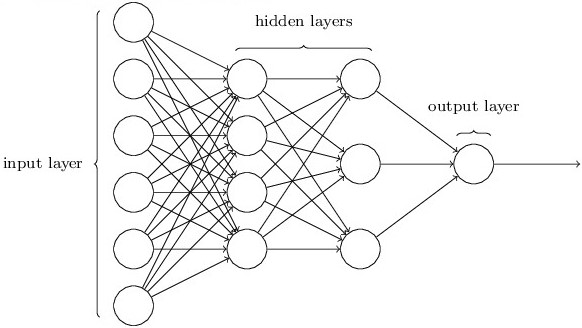
\includegraphics[scale=0.75]{Images/Experiments/ann_architecture.jpg}
    \caption{Four-layer neural network\cite{ann}.}
     \label{fig:ann}
\end{figure}

\subsection{Forward Propagation}
The phase of propagating an input vector through the network and getting an output is called \textit{forward propagation}. The \gls{ann} takes a vector as input which is passed to the input layer in \textbf{\autoref{fig:ann}}. The network can have one or several hidden layers after the input layer, each layer containing neurons. To get the output of a layer, the neurons or weights are multiplied by the input, and an activation function is applied to the result of the aforementioned computation.
%The number of neurons in the output layer equals the number of possible classifications. 
The output of the output layer will be the final prediction made by the \gls{ann}.\cite{ann} An activation function is applied in the layers of the \gls{ann} to introduce non-linearity. Without non-linear activation functions, several hidden layers do not make sense, as they do not add additional power compared to a single layer. Non-linear activation function also makes it possible to non-linearly map the input to the output, which is necessary for most real world application.%, which is also the reason for the \gls{ann} being called the universal function approximator. 
%to represent the value given by the node as preferred\cite{nnadl}. In this example, the node output is a probability. That is, a value between 0 and 1.
In the \gls{ann}, the output of the previous layer is given an input to the next layer, while the output of the output layer is the final prediction.%, known as \textit{feedforward} neural networks, where cycles are not allowed as in \textit{recurrent} neural networks.\cite{ann}

\subsection{Backpropagation}

The backpropagation algorithm is used for understanding how much the weights in a network contributes to the loss. When the network consists of multiple layers, the loss is a composition function of the weights in the earlier layers. The backpropagation algorithm is used to find the gradient of the composition function, which includes the magnitude and direction of the function. The algorithm uses the chain rule of differential calculus, which will compute the error gradient through summations of the local-gradient product over the different paths in the network from a node to the output. %This calculation can be done efficiently using dynamic programming, and the backpropagation algorithm is an application of dynamic programming. 

%The backpropagation includes two main phases: the forward phase and the backward phase.

The backpropagation includes two main steps: the forward pass to calculate loss and a backtracking step, which traverses backwards from the deeper layers to calculate the derivatives of the weights, with respect to the loss. The forward pass is calculated through forward propagation.
%In the forward phase, the training data is fed to the neural network, and a cascade of computations will happen throughout the layers using the current weights. The output from the training will be compared to the final predicted output, and the derivative of the loss function is computed. 
In the backwards phase, the goal is to use the chain rule to compute the gradient of the loss function, in respect to the different weights. The gradients can thereafter be used to update the weights, through gradient descent explained in the following section. In this way, we optimize the weights, so the neural network will gain knowledge of how to correctly map the inputs to the outputs of the neural network.\cite{nnadl}

\subsection{Gradient Descent}
Gradient Descent is an algorithm that updates weights and biases for neurons so that the output from the neural network approximates its prediction for all training inputs. The main idea is to find the weights and biases so that the cost, the \gls{mse}, is as small as possible. Minimising \gls{mse} makes it easier to change the weights and biases in order to improve performance compared to maximizing the number of correct detection outputs.\cite{ann}

We let \gls{mse} be a function defined as $C(v)$, where $v$ is a set of many variables. We can minimise the function $C(v)$ by finding where $C$, in the optimal case, achieves its global minimum. We find the minimum by computing derivatives of $C$, since this would tell us the slopes of the function, which in turn tells the minimum of $C$.\cite{ann}
\section{Long Short-Term Memory (LSTM)}

As mentioned in \textbf{\autoref{rnn1}}, there are different types of \gls{rnn}s, but the \gls{lstm} model is one of the most widely used in regards to \gls{ips}. We will therefore also use the \gls{lstm} structure for our experiment with \gls{rnn}.

In a recurrent network, the output from a previous step will be used as input for the next step. In an \gls{lstm} model, the nodes are recurrent, and they also include a cell state. This cell state is the working memory space which is used by the node, so the information can be stored and retrieved over multiple time steps. Therefore, in an \gls{lstm}, the input value, the previous output, and the cell state are all used in the calculations of the node. The results of this calculation are used to get an output value, but also to update the cell state. Besides from having parameters for defining how inputs should be used in the calculations, as in standard neural networks, the \gls{lstm}'s nodes also include gates. The gates are responsible for controlling the flow within the node, which especially includes determining how much of the saved information should be used in a given calculation. The gate parameters are made of weights and biases, and therefore, the input determines the behaviour. There are three types of gates in an \gls{lstm} network; the input gate, the forget gate and the output gate. The \gls{lstm} network can therefore be divided into three different parts, as shown in \textbf{\autoref{fig:lstm}}. 

\begin{figure}[H]
    \centering
    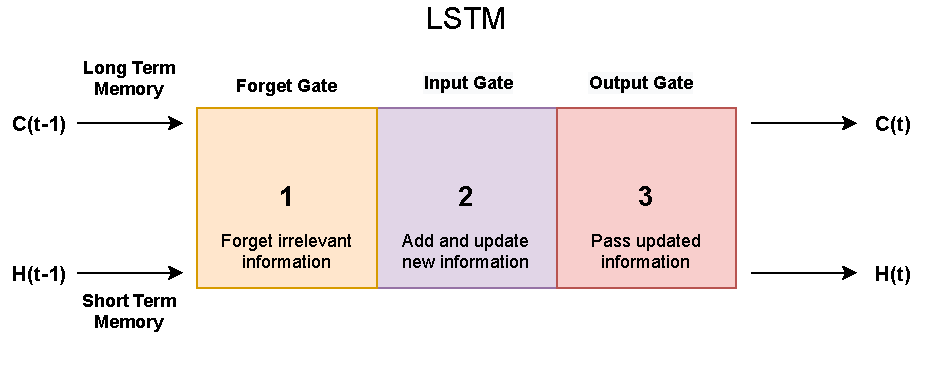
\includegraphics[scale=0.85]{Images/Experiments/lstm.pdf}
    \caption{Overview of an LSTM network.}
    \label{fig:lstm}
\end{figure}

In the first part of the \gls{lstm}, the network will try to determine whether the information from the previous timestamp is relevant or if it should be forgotten. In the second part, the cell will try to learn new information from the given input, and update the information. In the last step, the cell will pass the information that it has updated, from the current timestamp to the next timestamp. Besides from the cell state, the \gls{lstm} network also includes a hidden state, as known in standard \gls{rnn} networks. In \textbf{\autoref{fig:lstm}}, $H(t-1)$ denotes the hidden state of the previous timestamp, and $H(t)$ denotes the hidden state of the current timestamp. $C(t-1)$ and $C(t)$ denote the previous and current timestamps for the cell state, respectively. The cell state can be viewed as the long term memory of the system, and the hidden state can be seen as the short term memory. The information from the timestamps are used in the calculations in the different gates in the network.\cite{lstmVidhya}

The \gls{lstm} networks are less exposed to the vanishing gradient problem, mentioned in \textbf{\autoref{sec:vanishing_exploding_gradient_problem}}, but the exploding gradient problem can still be encountered. Another disadvantage of the \gls{lstm} is that they are very computational intensive.\cite{Yalcın2021}
\section{Problems with Machine Learning Models} \label{sec:problemsmachinelearning}
In this section, we will explore the disadvantages that can occur when working with machine learning models. Doing so will benefit to understand the problems and avoid mistakes.  

\subsection{Overfitting and Underfitting}\label{sec:over_underfit}

When working with machine learning, one of the biggest challenges is to create a model that is complex enough to solve hard problems, but not complex enough to misunderstand the concept. If the concept is too simple, we have a risk of underfitting. If the concept is too complex and only works for the training data, we have a risk of overfitting. In overfitting, the model is highly accurate on the training data, but would not generalise well, meaning that it would not perform well on unseen data. In underfitting, the model is often too simple, and will therefore struggle to identify the concept, and will therefore neither model the training data nor generalise to new data. It is therefore important to balance the complexity, so the model that is created produces the best generalisation.\cite{Hulten2018}

\subsection{Vanishing and Exploding Gradient Problem} \label{sec:vanishing_exploding_gradient_problem}

In \textbf{\autoref{neuralnetwork}}, the training of a neural network through gradient-based learning is described. When using gradients, there are different issues that can happen. The error gradient, which is used to update the weights in the network, can accumulate and result in a large gradient. Because of the large gradient, large updates to the weights will occur, and the network is in risk of being unstable. When the network is unstable, it may not learn from the training data, or result in Not A Number (NaN) weight values, which can not be updated. These large gradients are also referred to as exploding gradients.\cite{vanishingexploding}

Alternatively, we can also have derivatives that are too small, and the gradient will exponentially grow smaller when we propagate through the model, so we risk having a gradient that will vanish. This is referred to as the vanishing gradient problem.\cite{vanishingexploding}


\chapter{Experiments}
\section{Pedestrian Dead Reckoning} \label{sec:IMUPositioning_eval}
This section describes the evaluation of the \gls{pdr} algorithm using Madgwick orientation filter and Extended Kalman Filter for heading estimation.

%We will present a cumulative distribution graph of the evaluation results of the two experiments, one for each heading estimation filter. 
%Furthermore, 
An average positioning error has been computed of all positioning errors, but it is important to note that this value is highly affected by the length of each path in the evaluation. This is because the positioning error is accumulative for \gls{pdr}, as mentioned in \textbf{\autoref{sec:IMUPositioning}}. Therefore, the shorter a path in the evaluation is, the more the average positioning error is dragged towards a lower value, and therefore, this value does not truly represent the performance of a \gls{pdr} implementation of one heading estimation filter. However, the average positioning error can be used to compare the different \gls{pdr} implementations with the two different heading estimation filters, since both are evaluated on the same data and paths. Furthermore, the position errors of both filters for selected paths have been shown and evaluated on, as seen in \textbf{\autoref{PDR:results}}. The most remarkable diagrams are the diagrams shown in \textbf{\autoref{fig:pdr_performance}}. As it can be seen from the experiment results in \textbf{\autoref{PDR:results}}, the \gls{pdr} algorithm using Madgwick Filter for heading estimations performs best, since its positioning error is lower than the \gls{pdr} algorithm using Extended Kalman Filter for heading estimation. Furthermore, as explained in \textbf{\autoref{sec:IMUPositioning}}, the \gls{pdr} algorithm drifts the longer the path is, resulting in higher positioning errors per measurement. It is noticeable that the \gls{pdr} algorithm improves its estimations per measurement in \textbf{\autoref{fig:pdr_performance}(c)}. The reason for this might be that the \gls{pdr} algorithm makes three wrong heading estimations at measurement 748, 1654 and 2089 that turns the pedestrian toward the ground truth path.

The mean positioning errors across all paths for Madgwick and Extended Kalman Filter are 34.78 meters and 43.83 meters, respectively.

\begin{figure}[H]
\centering
\SetFigLayout{2}{2}
  \subfigure[]{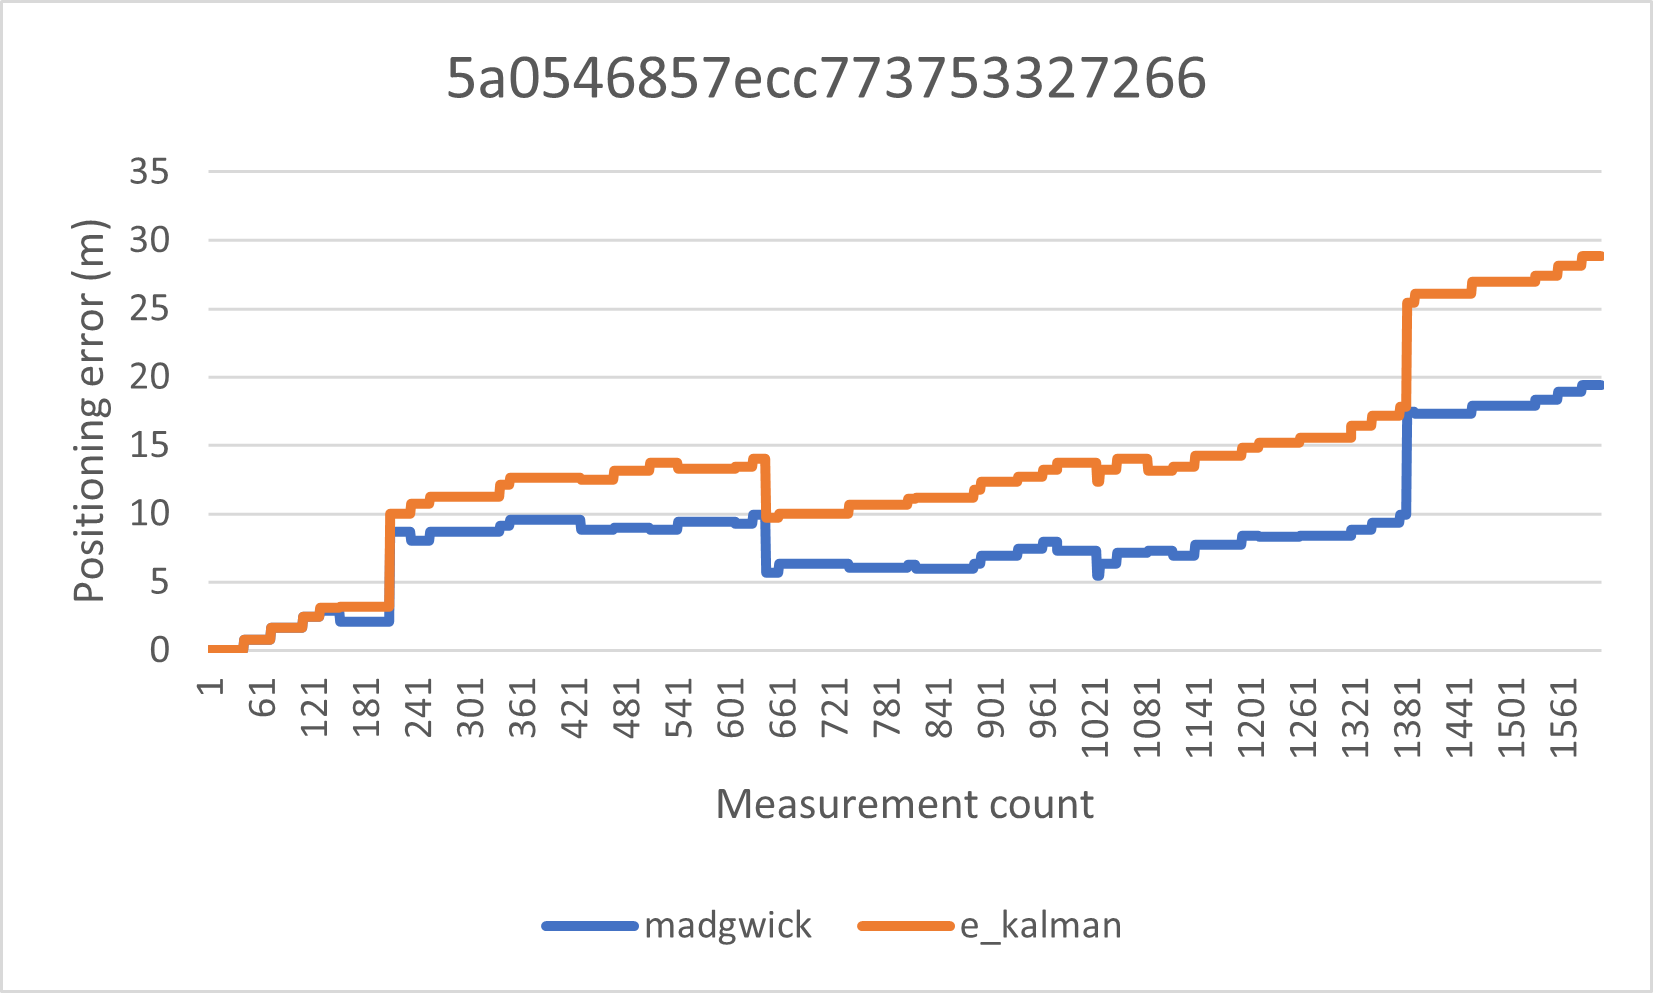
\includegraphics{Images/Experiments/pdr/pdr1.png}}
  \hfill
  \subfigure[]{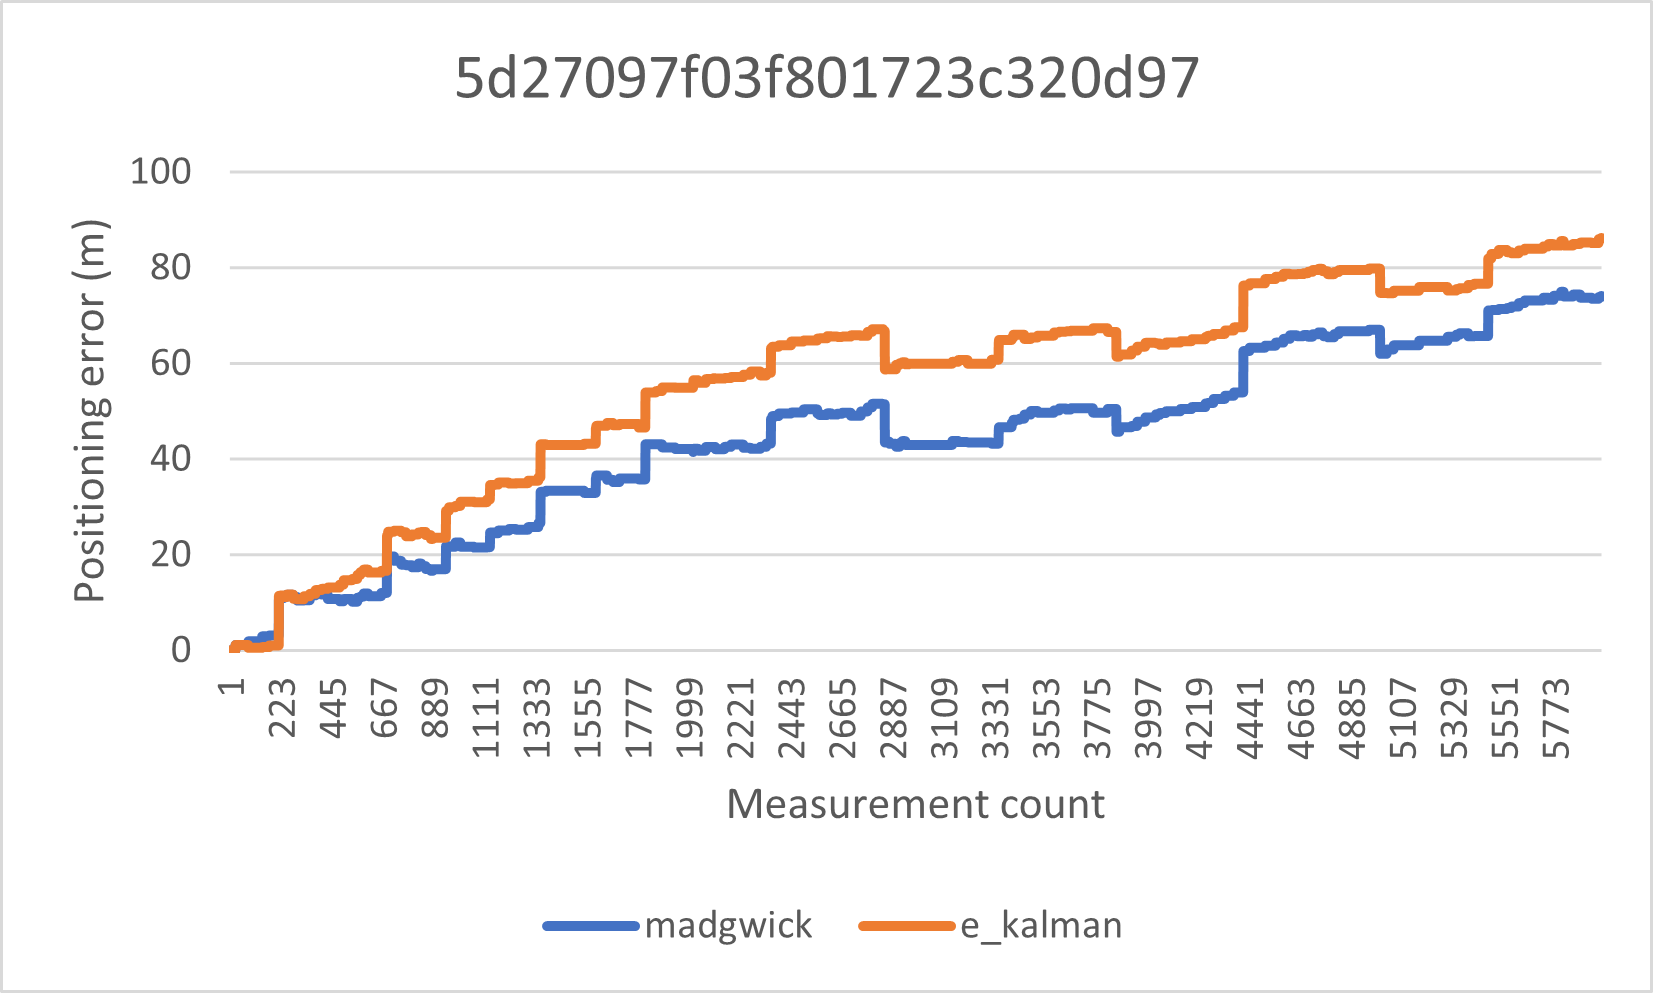
\includegraphics{Images/Experiments/pdr/pdr10.png}}
  \hfill
  \subfigure[]{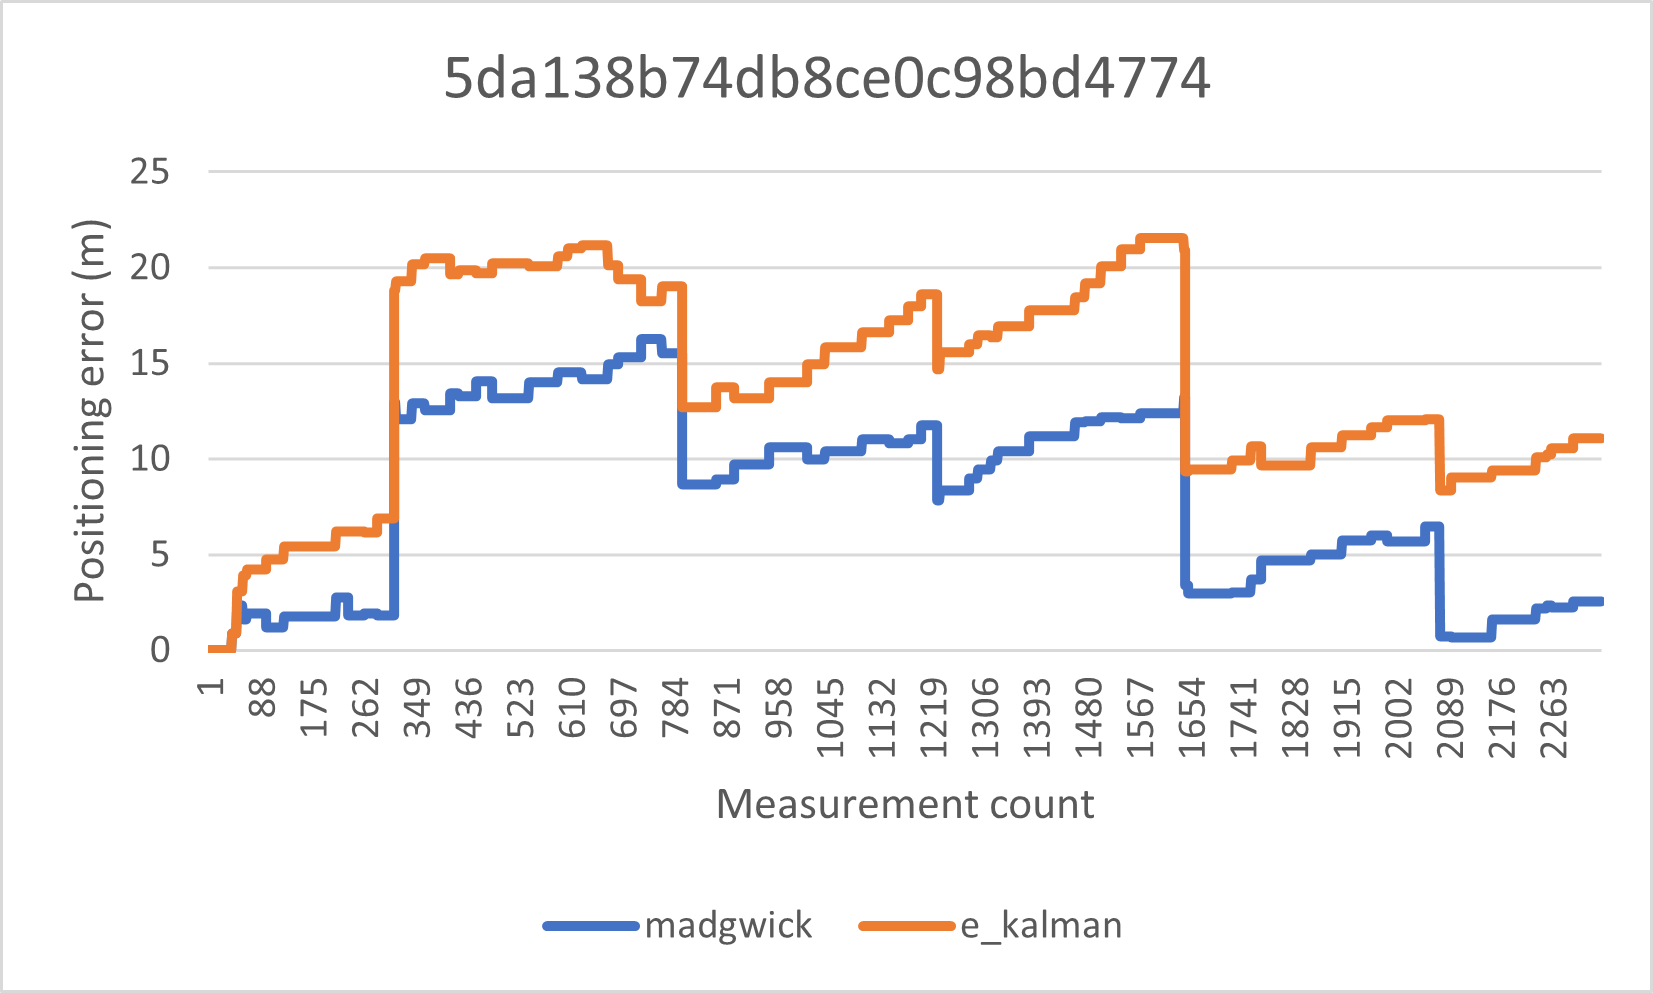
\includegraphics{Images/Experiments/pdr/pdr12.png}}
  \hfill
  \subfigure[]{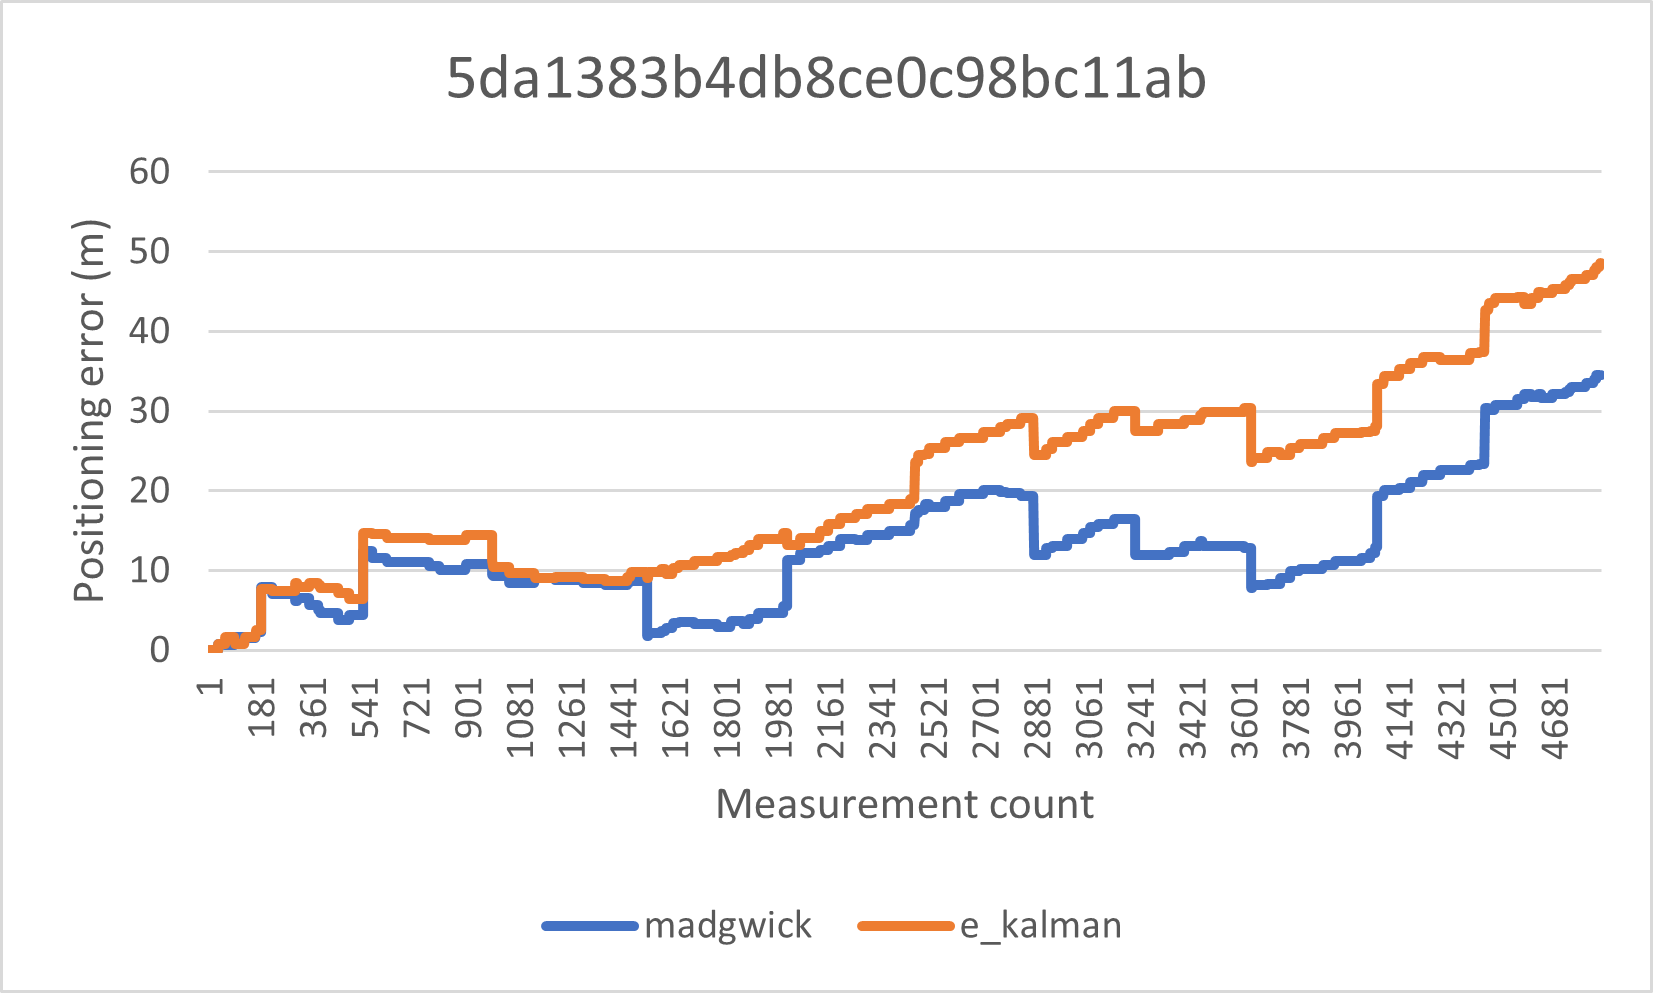
\includegraphics{Images/Experiments/pdr/pdr15.png}}
  \hfill
  \caption{\gls{pdr} performance using Madgwick Filter and Extended Kalman Filter for heading estimation.}
  \label{fig:pdr_performance}
\end{figure}

Furthermore, we have analysed the timestamps between the measurements. The longer the \gls{pdr} algorithm has to wait till next measurement, the more likely the position estimation is to be inaccurate. On \textbf{\autoref{fig:pdr_boxplot}} is seen a diagram that depicts the minimum, maximum and median variance in measurement timestamps.

\begin{figure}[H]
    \centering
    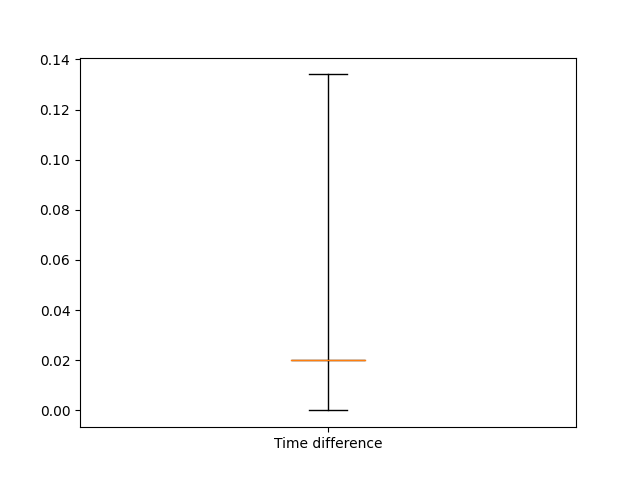
\includegraphics[scale = 0.55]{Images/Experiments/pdr/boxplot.png}
    \caption{Variance in measurement timestamps in seconds. The lowest line is the minimum timestamp difference, the middle line is the median and the highest line is the maximum.}
    \label{fig:pdr_boxplot}
\end{figure}

As seen on \textbf{\autoref{fig:pdr_boxplot}}, there is quite a difference from the median to the maximum measurement timestamp difference. The middle line consists of three lines; the median, 1st quartile and 3rd quartile. Because these three lines are so close to each other, it means that only a few of the measurement timestamps differ more than 0.02 from the previous measurement timestamp. These few measurement timestamps that differ more than 0.02 may be the reason to some of the major wrong heading estimations, since the heading estimation is based on receiving data with a given frequency. Therefore, these few measurement timestamps will temporarily decrease the expected frequency.

As seen on \textbf{\autoref{fig:pdr_cdf}}, it is clear that the Madgwick Filter implementation outperforms the Extended Kalman Filter implementation by their \gls{cdf}, since it can be seen in \textbf{\autoref{fig:pdr_cdf}(b)} that positioning errors using Extended Kalman Filter reach higher position error values with 565.02 meters for 100\% of the data compared to using Madgwick Filter with a positioning error of 400.40 meters for 100 \% of the data, seen in \textbf{\autoref{fig:pdr_cdf}(a)}. Furthermore, the positive slope of \gls{cdf} decreases at positioning error around 50 meters for \textbf{\autoref{fig:pdr_cdf}(a)}, whereas this does not happen until at around 100 meters for \textbf{\autoref{fig:pdr_cdf}(b)}. This generally means that the Extended Kalman Filter implementation outputs position estimations that are further off the ground truth position compared to the Madgwick Filter implementation.

\begin{figure}[H]
\centering
  \SetFigLayout{1}{2}
  \subfigure[]{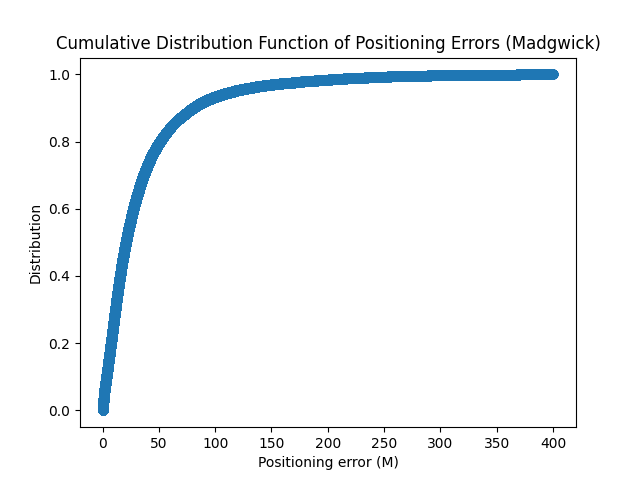
\includegraphics{Images/Experiments/pdr/cdf_madgwick.png}}
  \hfill
  \subfigure[]{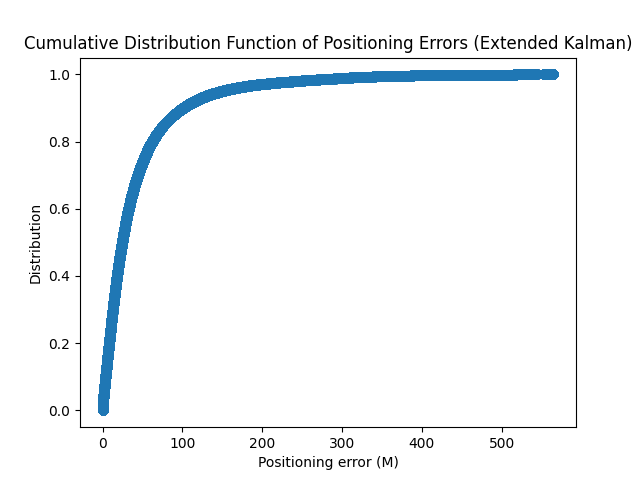
\includegraphics{Images/Experiments/pdr/cdf_kalman.png}}
  \caption{\gls{cdf} for Madgwick Filter implementation (a) and Extended Kalman Filter implementation (b).}
  \label{fig:pdr_cdf}
\end{figure}

Because the \gls{pdr} algorithm performs best using Madgwick Filter, this will be our choice of heading estimation filter for the algorithm.
\section{Artificial Neural Network} 
In this section, we will describe and reflect upon the result of the \gls{ann} experiments conducted in this project. We will also evaluate the performance of the \gls{ann} architecture proposed by \cite{} as we mentioned in \textbf{\autoref{}}. For the evaluation of the 
 
\subsection{Initial Model}
Initially, we have tested a variety of models, and we end up with the following initial model, which comparatively speaking performs well.
For our initial model, we have tested a model with the following specification:

\begin{table}[H]
    \centering
    \caption{Model Specification for initial \gls{ann} experiment.}
    \begin{tabular}{m{0.3\textwidth}m{0.2\textwidth} m{0.2\textwidth}}
        \hline
        \multicolumn{1}{c}{\textbf{Description}} & \multicolumn{1}{c}{\textbf{Neurons}} & \multicolumn{1}{c}{\textbf{Activation}}\\
        \hline
        
        Input Layer         &   \multicolumn{1}{c}{$N$} & \multicolumn{1}{c}{None}        \\
        1. Hidden Layer     &   \multicolumn{1}{c}{$\frac{1}{4}N$}  & \multicolumn{1}{c}{ReLU}     \\
        2. Hidden Layer     &   \multicolumn{1}{c}{$\frac{1}{2}N$}  & \multicolumn{1}{c}{ReLU}     \\
        Output Layer     &   \multicolumn{1}{c}{$1$}  & \multicolumn{1}{c}{None}     \\
        \hline
    \end{tabular}
    \label{tab:NN01}
\end{table}

% \begin{itemize}
%     \item A hidden layer with neurons amounting to half of the input neurons and relu activation function
%     \item A hidden layer with neurons amounting to $1/4$ of the input neurons and relu activation function
%     \item A hidden layer with neurons amounting to half of the input neurons and relu activation function
%     \item A output layer with one neuron
%     \item As gradient descent, Adam has been used with a learning rate of 0.01 in a batch size of 32.
% \end{itemize}
Models with the specification mentioned in \textbf{\autoref{tab:NN01}} have been trained for each site and for each X, Y, and floor. We have decided to implement models for X, Y, and floor separately as we believe that a more specific model will have better performance as it does not need to focus on more than one prediction. The models have been trained with the optimiser Adam, which is a variation of stochastic gradient descent, and in batches of size 32. The models have been trained for 100 epochs, but with early stopping with patience of 10 epoch in the validation loss. This means that if the validation loss does not improve in 10 epochs, the training of the model will end.

\subsubsection{Results of First Test}
The results of this model specification varies depending on the whether the prediction is X,Y or floor. We will evaluate each of them respectively. For the Y-values, when looking at the development of the training and validation loss, we can see that for most of the cases the initial loss is high. This can be seen on (a) on \textbf{\autoref{fig:NN01}}. Even when investigating the training after the initial training period, we can still see that the model struggles to find the optimal state and the final loss furthermore also seems to be quite high. This is indicated on (b) on \textbf{\autoref{fig:NN01}}. Furthermore, the mean of the \gls{mse}s for all sites for the training data and validation data are at 9372 and 2407.32, respectively. This further illustrates the issue of not finding an optima. 

\begin{figure}[H]
\centering
  \SetFigLayout{1}{2}
  \subfigure[]{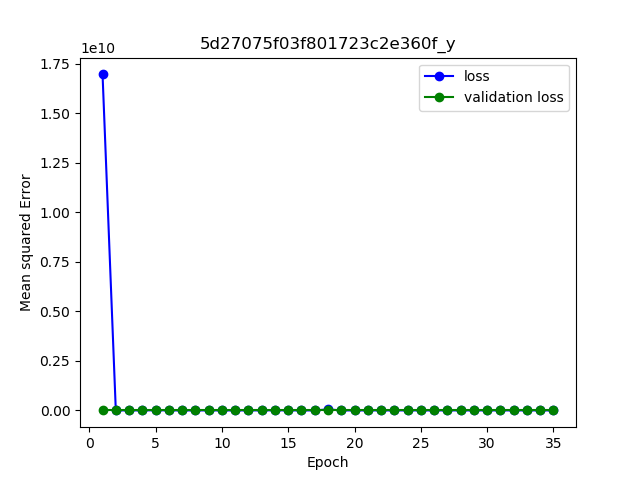
\includegraphics{Images/Experiments/NN/1.initial/all/5d27075f03f801723c2e360f_y.png}
  }
  \hfill
  \subfigure[]{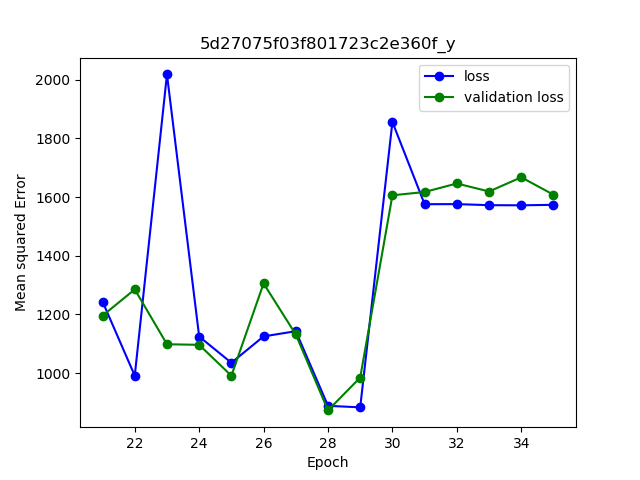
\includegraphics{Images/Experiments/NN/1.initial/after20/5d27075f03f801723c2e360f_y.png}}
  \caption{The performance for a site.}
  \label{fig:NN01}
\end{figure}
% \begin{figure}[h]
%     \centering
%     \includegraphics[scale=0.5]{Images/Experiments/NN/expr01/5da138764db8ce0c98bcaa46_y(0).png}
%     \caption{Training with all epochs}
%     \label{fig:NN_01}
% \end{figure}
% \begin{figure}[h]
%     \centering
%     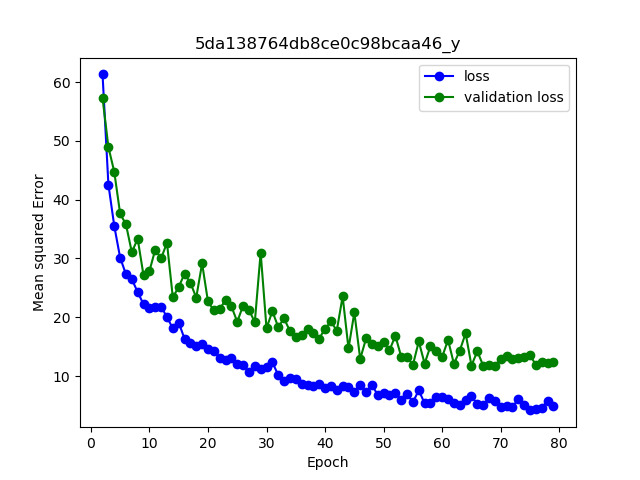
\includegraphics[scale=0.5]{Images/Experiments/NN/expr01/5da138764db8ce0c98bcaa46_y.png}
%     \caption{Training with epoch 2 and onward}
%     \label{fig:NN_02}
% \end{figure}
As with Y, we notice the same tendencies with results for the X predictions. The result of the same site as in \textbf{\autoref{fig:NN01}} is shown for the result for X estimations in \textbf{\autoref{fig:NN01_x}}. The mean of the \gls{mse}s for the sites for the X estimations are at 4967 and 3077 for the training and validation datasets, respectively.
\begin{figure}[H]
    \centering
    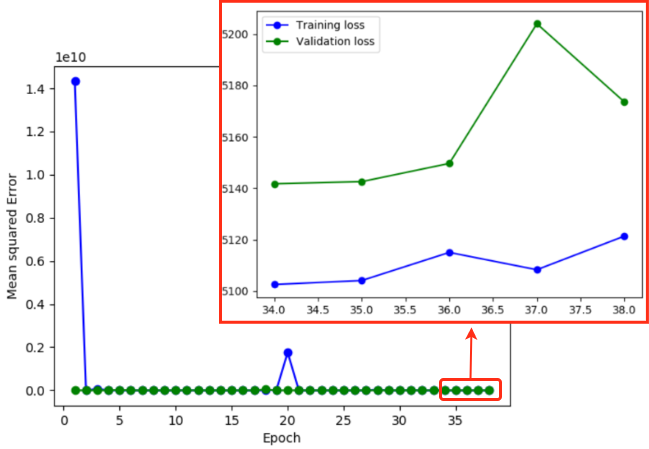
\includegraphics[scale=0.4]{Images/Experiments/NN/1.initial/5d27075f03f801723c2e360f_x.png}
    \caption{Results for site 5d27075f03f801723c2e360f for X estimations.}
    \label{fig:NN01_x}
\end{figure}
Among the estimations, we observe the worst behaviour for the floor estimations, when considering the mean of \gls{mse}s, which are at $166586.22$ and $8538.34$ for the training and validation data, respectively. However, for most of the sites for the floor predictions, we achieve good results, but the overall mean is dragged up due to a few extreme results. One of the good results is displayed in \textbf{\autoref{fig:NN01_floor}}.
\begin{figure}[H]
    \centering
    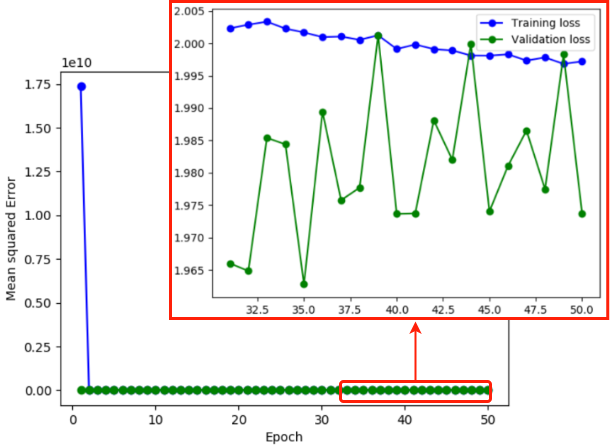
\includegraphics[scale=0.4]{Images/Experiments/NN/1.initial/5d27075f03f801723c2e360f_floor.png}
    \caption{Results for site 5d27075f03f801723c2e360f for floor estimations.}
    \label{fig:NN01_floor}
\end{figure}

The overall issue with struggling to find the optima, which we observe especially for the X and Y estimations, can have a number of reasons. The reasoning for this, which we think is most likely, might be due to a high learning rate or due to the model being unable to properly localise the optimum in the raw dataset. To this end, we will try to decrease the learning rate in one experiment and try training with the normalised dataset in another experiment.


\subsubsection{Results of Second Test}
After conducting the experiment with an adjusted learning rate of 0.001, we achieve better results compared to the initial experiment for all the models. This is deemed from the mean of \gls{mse}s on both training and validation dataset. 

%The results for the site, which we have shown for the earlier experiment, is shown here. 
%In the initial experiment, we end up with a loss around 1600, while in with the adjusted learning rate we achieve a loss around 50. This is further illustrated by the mean of the \gls{mse}s on the training and validation dataset, which is 1590 and 2191 for the initial experiment, while it becomes 516 and 475 for the second experiment for the training and validation \gls{mse}s, respectively.
% \begin{figure}[H]
% \centering
%   \SetFigLayout{1}{2}
%   \subfigure[]{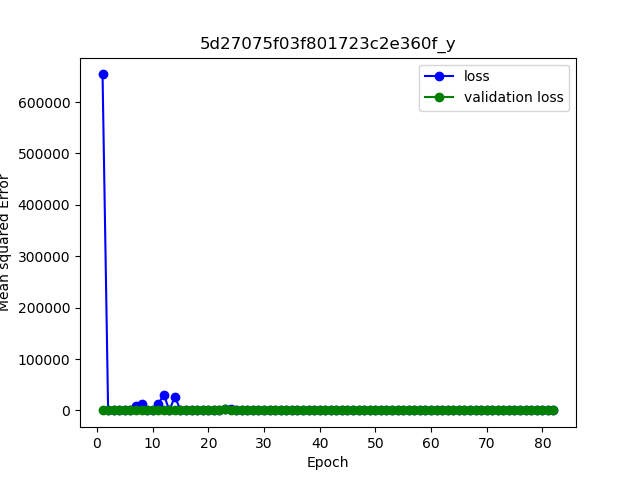
\includegraphics{Images/Experiments/NN/2.adjustedLR/5d27075f03f801723c2e360f_y_all.png}
%   }
%   \hfill
%   \subfigure[]{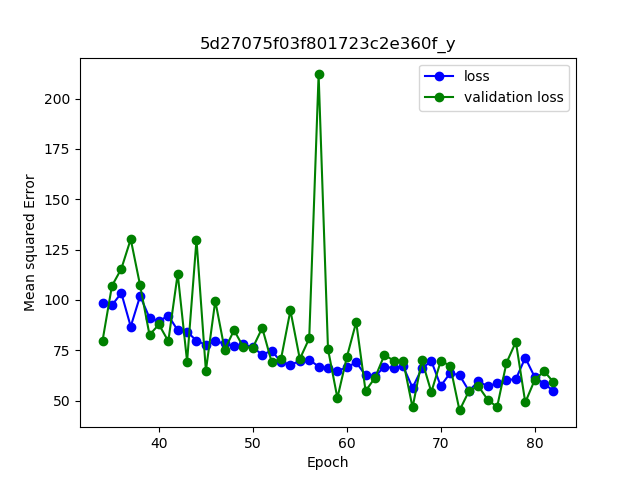
\includegraphics{Images/Experiments/NN/2.adjustedLR/5d27075f03f801723c2e360f_y_34.png}
%   }
%   \caption{The performance for a site.}
%   \label{fig:NN02}
% \end{figure}
\begin{figure}[H]
\centering
  \SetFigLayout{1}{2}
  \subfigure[]{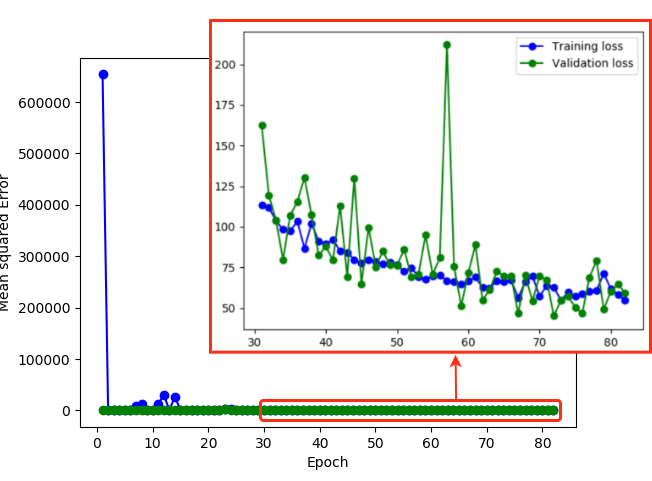
\includegraphics{Images/Experiments/NN/1.initial/exp2_y_5d27075f03f801723c2e360f.png}
  }
  \hfill
  \subfigure[]{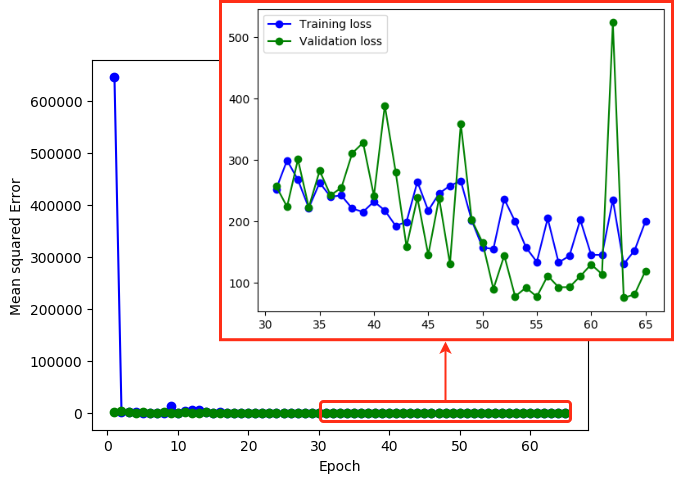
\includegraphics{Images/Experiments/NN/1.initial/exp2_x_5d27075f03f801723c2e360f.png}}
  \caption{Results for site 5d27075f03f801723c2e360f for y estimations (a) and x estimations (b).}
  \label{fig:exp2}
\end{figure}

\textbf{\autoref{fig:exp2}} displays the result of the X and Y estimations. For the X estimations, the mean of \gls{mse}s are 669 \& 2298.73 for training and validation, respectively. This is still a quite huge gap between the training and validation loss. For the Y estimations, we achieve a mean of \gls{mse}s of 1159 for training and 230.59 for validation.  Lastly for the Floor model, we achieve 8891 for training dataset and 533.03 for validation dataset. We see an improvement in comparison to the initial test, but overall the performance still does not seem ideal.

%\begin{figure}[H]
   % \centering
   % \includegraphics[scale=0.5]{Images/Experiments/NN/1.initial/e%xp2_floor_5d27075f03f801723c2e360f.png}
   % \caption{Results for site 5d27075f03f801723c2e360f for floor %estimations.}
   % \label{fig:exp2_floor}
%\end{figure}

\subsubsection{Results of Third Test}
We have also conducted the experiment with a normalised dataset. The data is normalised through Min-Max Normalisation, which is used to scale features as mentioned in \autoref{sec:minmaxnormalisation}. Applying this to the \gls{ann} model should lead to a decrease in the loss and an increase in the performance of the model.

\begin{figure}[H]
\centering
  \SetFigLayout{1}{2}
  \subfigure[]{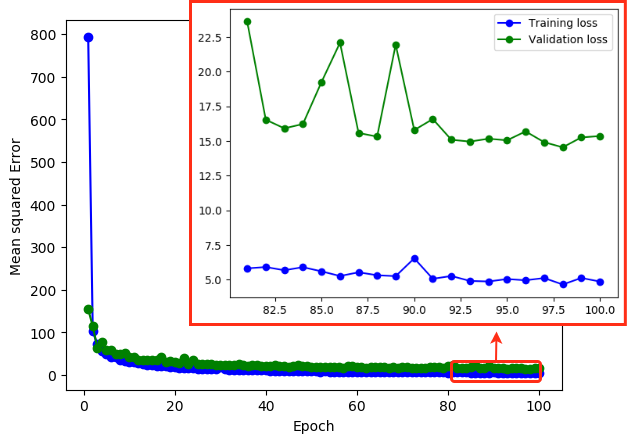
\includegraphics{Images/Experiments/NN/1.initial/exp3_y_5d27075f03f801723c2e360f.png}
  }
  \hfill
  \subfigure[]{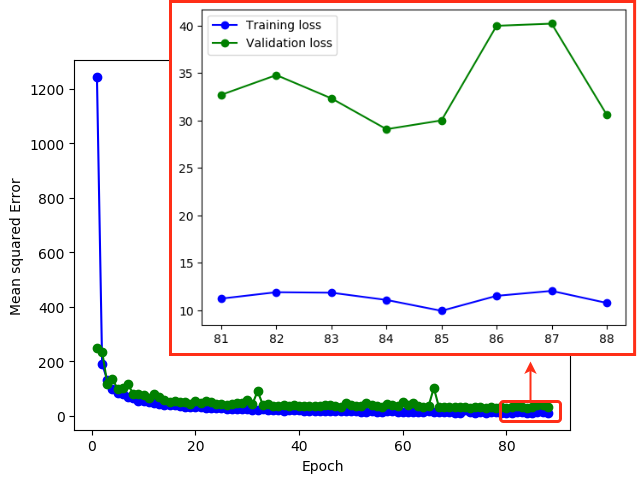
\includegraphics{Images/Experiments/NN/1.initial/exp3_x_5d27075f03f801723c2e360f.png}}
  \caption{Results for site 5d27075f03f801723c2e360f for y estimations (a) and x estimations (b).}
  \label{fig:exp3}
\end{figure}

After using the normalised data instead, the mean of \gls{mse}s dropped significantly, which can be seen on \textbf{\autoref{fig:exp3}}. The \textit{X} model has dropped from a mean of \gls{mse}s from 4967 on the initial model to 10.41 on the training data. The \textit{Y} model has decreased from a mean of \gls{mse}s from 9372 on the initial model to 8.98 on the training data. As can be seen from the graphs, the validation loss is quite high compared to the training loss, which is not an issue of same degree with adjusting the learning rate.

%\begin{figure}[H]
    %\centering
    %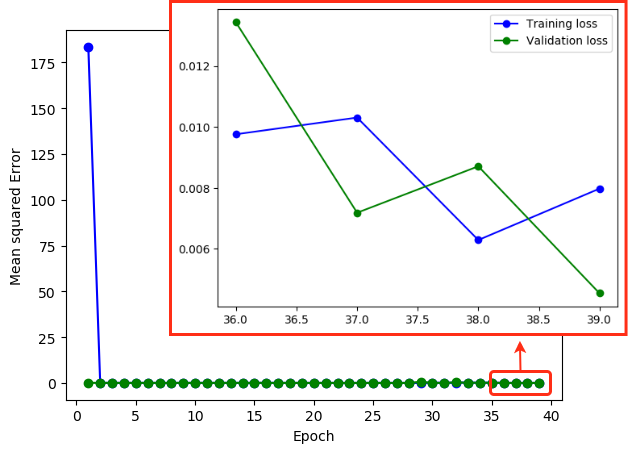
\includegraphics[scale=0.5]{Images/Experiments/NN/1.initial/exp3_floor_5d27075f03f801723c2e360f.png}
    %\caption{Results for site 5d27075f03f801723c2e360f for floor estimations.}
    %\label{fig:exp3_floor}
%\end{figure}
%Here we get a mean on \gls{mse}s for training and validation of 5.6 and 14.9, respectively. The loss is significantly less compared to the previous experiments. 

The most significant change is in the \textit{Floor} model, which decreases the mean of \gls{mse}s to 0.034 for the training dataset and 0.0334 for validation dataset. This proves the assumption about the data making the model unable to properly localise the optimum. Since both reducing the learning rate and using the normalised data combined might lead to even better results. 


\subsection{Result of Fourth Test}
We have also tried a combination of min-max normalised dataset as well as less learning rate, which seems to give good performance. 

\begin{figure}[H]
\centering
  \SetFigLayout{1}{2}
  \subfigure[]{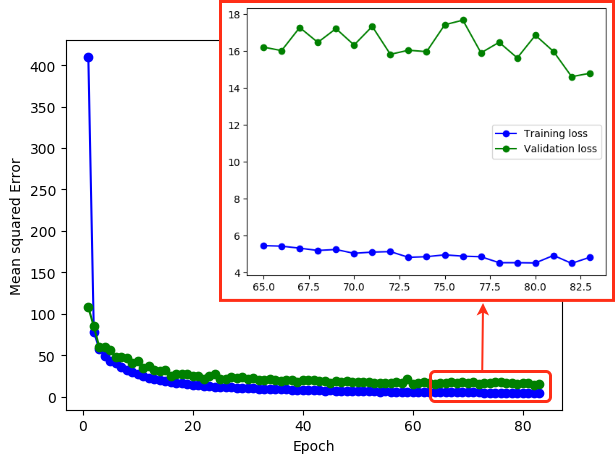
\includegraphics{Images/Experiments/NN/1.initial/exp4_y_5d27075f03f801723c2e360f.png}
  }
  \hfill
  \subfigure[]{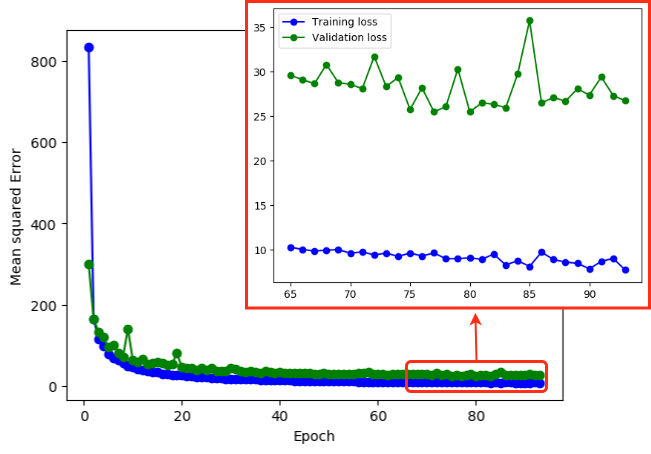
\includegraphics{Images/Experiments/NN/1.initial/exp4_x_5d27075f03f801723c2e360f.png}}
  \caption{Results for site 5d27075f03f801723c2e360f for y estimations (a) and x estimations (b).}
  \label{fig:exp4}
\end{figure}

This for the X and Y model resulted in losses as displayed in \textbf{\autoref{fig:exp3}}, which displays quite a decrease in loss compared to the prior experiments. The graphs seem to perform a bit worse on the validation dataset than for the training dataset, which could be due to slight overfitting.

\begin{figure}[H]
    \centering
    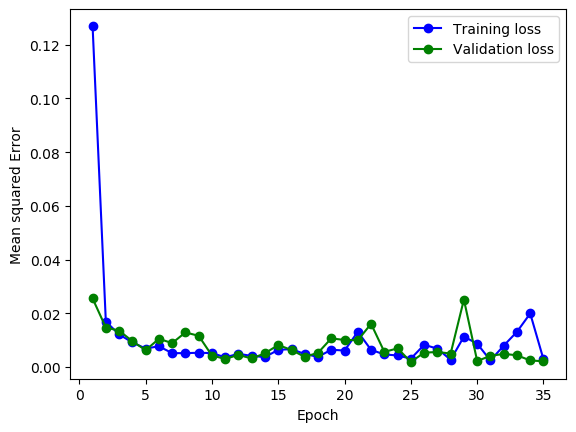
\includegraphics[scale=0.5]{Images/Experiments/NN/1.initial/exp4_floor_5d27075f03f801723c2e360f.png}
    \caption{Results for site 5d27075f03f801723c2e360f for floor estimations.}
    \label{fig:exp4_floor}
\end{figure}

For the \textit{Floor} model, the performance has increased severely since the initial model. The final mean of \gls{mse}s for the training set is 0.0019 and for the validation set is 0.0027.

%We have also calculated the mean of the \gls{mse} for training data and test data is 4.4 and 12.2, respectively. The result, which we achieve for the normalised and less learning rate, seem to perform the best.




\subsubsection{Evaluation of Initial Model}
To evaluate the initial model, we use the \gls{mse}. After determining the most optimal hyper parameters, the k for k-fold should be determined. On \textbf{\autoref{tab:NN_train_initial_results}} and \textbf{\autoref{tab:NN_val_initial_results}}, we see the results for the training data and validation data for the three models (\textit{X}, \textit{Y} and \textit{Floor}). Each model is decribed by the best of k \gls{mse}s, the mean of the \gls{mse}s and the worst of k \gls{mse}s.

\begin{table}[H]
    \centering
    \caption{Results of the training dataset for initial \gls{ann} models, where \textbf{B} stands for the best of k \gls{mse}s, while \textbf{M} stands for the mean of the \gls{mse}s, and \textbf{W} stands for the worst.}
    \begin{adjustbox}{max width=\textwidth}
    \begin{tabular}{m{0.15\textwidth}@{\extracolsep{0.1cm}} m{0.05\textwidth}@{\extracolsep{0pt}} m{0.05\textwidth} m{0.05\textwidth} @{\extracolsep{0.1cm}} m{0.05\textwidth}
    @{\extracolsep{0pt}}
    m{0.05\textwidth} m{0.05\textwidth} @{\extracolsep{0.1cm}} m{0.05\textwidth}@{\extracolsep{0pt}} m{0.05\textwidth} m{0.05\textwidth}}
        \hline
         \multirow{2}{*}{\centering
         \textbf{Description}} & \multicolumn{3}{c}{\textbf{X}} & \multicolumn{3}{c}{\textbf{Y}}& \multicolumn{3}{c}{\textbf{Floor}}\\
         \cline{2-10}
         & \multicolumn{1}{c}{\textbf{B}} & \multicolumn{1}{c}{\textbf{M}}& \multicolumn{1}{c}{\textbf{W}}& \multicolumn{1}{c}{\textbf{B}}& \multicolumn{1}{c}{\textbf{M}}& \multicolumn{1}{c}{\textbf{W}}& \multicolumn{1}{c}{\textbf{B}}& \multicolumn{1}{c}{\textbf{M}}& \multicolumn{1}{c}{\textbf{W}}\\
        \hline\\
        Initial Model & \multicolumn{1}{c}{1073} & \multicolumn{1}{c}{4967} & \multicolumn{1}{c}{$3.1\cdot10^{4}$} & \multicolumn{1}{c}{731} & \multicolumn{1}{c}{9372} & \multicolumn{1}{c}{$7.3\cdot10^{4}$} & \multicolumn{1}{c}{2.67} & \multicolumn{1}{c}{$1.6\cdot10^{5}$} & \multicolumn{1}{c}{$1.6\cdot10^{6}$}
        \\\\
        %\\\hline\\
        Adjusted LR & \multicolumn{1}{c}{72.38} & \multicolumn{1}{c}{669} & \multicolumn{1}{c}{5414} & \multicolumn{1}{c}{77.30} & \multicolumn{1}{c}{1159} & \multicolumn{1}{c}{807} & \multicolumn{1}{c}{1.25} & \multicolumn{1}{c}{8891} & \multicolumn{1}{c}{79966}
        \\\\
        %\\\hline\\
        Normalised Data & \multicolumn{1}{c}{8.03} & \multicolumn{1}{c}{10.41} & \multicolumn{1}{c}{15.89} & \multicolumn{1}{c}{6.75} & \multicolumn{1}{c}{8.98} & \multicolumn{1}{c}{11.63} & \multicolumn{1}{c}{$9.3\cdot 10^{-4}$} & \multicolumn{1}{c}{0.034} & \multicolumn{1}{c}{0.25}
        \\\\
        %\\\hline\\
        Adjusted LR \& Normalised Data & \multicolumn{1}{c}{5.41} & \multicolumn{1}{c}{7.45} & \multicolumn{1}{c}{9.40} & \multicolumn{1}{c}{4.87} & \multicolumn{1}{c}{6.47} & \multicolumn{1}{c}{7.25} & \multicolumn{1}{c}{$9.5\cdot 10^{-4}$} & \multicolumn{1}{c}{0.0019} & \multicolumn{1}{c}{0.0047}
        \\\hline
    \end{tabular}
    \end{adjustbox}
    \label{tab:NN_train_initial_results}
\end{table}

\textbf{\autoref{tab:NN_train_initial_results}} displays the \gls{mse}s for the training dataset. The first row displays information about the initial model before adjusting the learning rate and using the normalised data. Especially, using the normalised data decreases the \gls{mse}s for all the models with both best and worst k \gls{mse}s. Last row describes the model after both adjusting the learning rate and using the normalised data. This model clearly decreases the \gls{mse}s compared to the previous models. The \textit{X} model has decreased from a mean of \gls{mse}s of 4967 to 7.45, and the \textit{Y} model has decreased from a mean of \gls{mse}s of 9372 to 6.47. The model for predicting floors has decreased extremely from a mean of \gls{mse}s of 160000 to 0.0019.

\begin{table}[H]
    \centering
    \caption{Results of the validation dataset for initial \gls{ann} models, where \textbf{B} stands for the best of k \gls{mse}s, while \textbf{M} stands for the mean of the \gls{mse}s, and \textbf{W} stands for the worst.}
    \begin{adjustbox}{max width=\textwidth}
    \begin{tabular}{m{0.15\textwidth}@{\extracolsep{0.1cm}} m{0.05\textwidth}@{\extracolsep{0pt}} m{0.05\textwidth} m{0.05\textwidth} @{\extracolsep{0.1cm}} m{0.05\textwidth}
    @{\extracolsep{0pt}}
    m{0.05\textwidth} m{0.05\textwidth} @{\extracolsep{0.1cm}} m{0.05\textwidth}@{\extracolsep{0pt}} m{0.05\textwidth} m{0.05\textwidth}}
        \hline
         \multirow{2}{*}{\centering
         \textbf{Description}} & \multicolumn{3}{c}{\textbf{X}} & \multicolumn{3}{c}{\textbf{Y}}& \multicolumn{3}{c}{\textbf{Floor}}\\
         \cline{2-10}
         & \multicolumn{1}{c}{\textbf{B}} & \multicolumn{1}{c}{\textbf{M}}& \multicolumn{1}{c}{\textbf{W}}& \multicolumn{1}{c}{\textbf{B}}& \multicolumn{1}{c}{\textbf{M}}& \multicolumn{1}{c}{\textbf{W}}& \multicolumn{1}{c}{\textbf{B}}& \multicolumn{1}{c}{\textbf{M}}& \multicolumn{1}{c}{\textbf{W}}\\
        \hline\\
        Initial Model & \multicolumn{1}{c}{780.27} & \multicolumn{1}{c}{3077.49} & \multicolumn{1}{c}{13291.79} & \multicolumn{1}{c}{681.45} & \multicolumn{1}{c}{2407.32} & \multicolumn{1}{c}{7130.71} & \multicolumn{1}{c}{2.02} & \multicolumn{1}{c}{8538.34} & \multicolumn{1}{c}{$85035.24$}
        \\\\
        %\\\hline\\
        Adjusted LR & \multicolumn{1}{c}{62.50} & \multicolumn{1}{c}{2298.73} & \multicolumn{1}{c}{5413.96} & \multicolumn{1}{c}{57.66} & \multicolumn{1}{c}{230.59} & \multicolumn{1}{c}{966.00} & \multicolumn{1}{c}{0.81} & \multicolumn{1}{c}{533.03} & \multicolumn{1}{c}{5300.95}
        \\\\
        %\\\hline\\
        Normalised Data & \multicolumn{1}{c}{14.57} & \multicolumn{1}{c}{21.21} & \multicolumn{1}{c}{39.74} & \multicolumn{1}{c}{12.31} & \multicolumn{1}{c}{19.74} & \multicolumn{1}{c}{41.58} & \multicolumn{1}{c}{0.00094} & \multicolumn{1}{c}{0.0334} & \multicolumn{1}{c}{0.25}
        \\\\
        %\\\hline\\
        Adjusted LR \& Normalised Data & \multicolumn{1}{c}{12.26} & \multicolumn{1}{c}{17.29} & \multicolumn{1}{c}{26.54} & \multicolumn{1}{c}{10.90} & \multicolumn{1}{c}{14.41} & \multicolumn{1}{c}{19.13} & \multicolumn{1}{c}{0.00041} & \multicolumn{1}{c}{0.0027} & \multicolumn{1}{c}{0.014}
        \\\hline
    \end{tabular}
    \end{adjustbox}
    \label{tab:NN_val_initial_results}
\end{table}

\textbf{\autoref{tab:NN_val_initial_results}} displays the \gls{mse}s for the validation dataset. The different \gls{mse}s follow similar values to the \gls{mse}s training data in \textbf{\autoref{tab:NN_train_initial_results}}. Similarly, adjusting the learning rate and using the normalised data has decreased the models for \textit{X}, \textit{Y} and \textit{Floor} respectively to 17.29, 14.41 and 0.0027. The mean of the \gls{mse}s for the Floor model is quite similar from training and validation. Where the models for \textit{X} and \textit{Y} increases the mean of \gls{mse}s by 9.84 and 7.94 respectively for validation. This increase could potentially mean that the model is slightly overfitting, since it performs worse on the validation data.

In general, for all of the initial \gls{ann} experiments, none of them have a high degree of overfitting. Meaning that the model does not over specialise for the training data and thereby get good results for the training data while getting bad results for the validation data. This might be an indication of the initial model might not have enough expressive power. So for the next model, we will try to increase the expressive power of the model.

\subsection{Second Model}
We have also experimented with a deeper model. 
\begin{table}[H]
    \centering
    \caption{Model Specification for a deeper \gls{ann} experiment.}
    \begin{tabular}{m{0.3\textwidth}m{0.2\textwidth} m{0.2\textwidth}}
        \hline
        \multicolumn{1}{c}{\textbf{Description}} & \multicolumn{1}{c}{\textbf{Neurons}} & \multicolumn{1}{c}{\textbf{Activation}}\\
        \hline
        
        Input Layer         &   \multicolumn{1}{c}{$N$} & \multicolumn{1}{c}{None}        \\
        1. Hidden Layer     &   \multicolumn{1}{c}{$N$}  & \multicolumn{1}{c}{ReLU}     \\
        2. Hidden Layer     &   \multicolumn{1}{c}{$\frac{1}{2}N$}  & \multicolumn{1}{c}{ReLU}     \\
        3. Hidden Layer         &   \multicolumn{1}{c}{$\frac{1}{2}N$} & \multicolumn{1}{c}{ReLU}        \\
        4. Hidden Layer         &   \multicolumn{1}{c}{$\frac{1}{2}N$} & \multicolumn{1}{c}{ReLU}        \\
        5. Hidden Layer         &   \multicolumn{1}{c}{$\frac{1}{4}N$} & \multicolumn{1}{c}{ReLU}        \\
        Output Layer     &   \multicolumn{1}{c}{$1$}  & \multicolumn{1}{c}{None}     \\
        \hline
    \end{tabular}
    \label{tab:NN02}
\end{table}
We have trained this model using the normalised dataset. For X estimations, we achieves mean of \gls{mse}s of 124.72 and 18.65 for training and validation dataset. The best of k mean of \gls{mse}s for X estimations are 5.89 and 10.85 for training and validation, while the worst of k mean of \gls{mse}s are 532.67 and 31.76.

For Y estimations, we achieve a mean of \gls{mse}s of 13.08 and 115.10 for training and validation, respectively. For the best k mean of \gls{mse}s, we get 5.94 \& 11.08 for training and validation, respectively, while we get 33.61 and 520.30 of the worst k.

For the floor estimations, we achieve a mean of \gls{mse}s of 5.54 and 0.99 for the training and validation. For the best k mean of \gls{mse}s, we get 0.23 and 0.21, while we get for the worst 3.27 and 2.39 for training and validation.

So looking at the results overall, it does not seem to be an improvement compared to the initial models. Perhaps with further testing of increasingly deep model, we might get a good performance, but due to time constraints we cannot keep testing models.


\subsection{Reflection on Experiments}
\todo{Abi ved hvad der menes, så han fixer :) -flet ind således at det står imellem intial model og second model}
%In general, for all of the \gls{ann} experiments, none of them have a high degree of overfitting. Meaning that the model does not over specialise for the training data and thereby get good results for the training data while getting bad results for the validation data. This might be an indication of the initial model might not have enough expressive power. So for the next model, we will try to increase the expressive power of the model. 
The training time with 10-fold cross validation is long, so we would like to test with 5-fold cross validation. If we do not identify a big difference in performance, we will be using 5-fold cross validation. 
%The mean of \gls{mse}s for training and validation data for 5-fold cross validation is 4.6 and 13.3, respectively. As this difference is minor compared to the 10-fold cross validation, we will be using 5-fold henceforth in order to save training time.

\chapter{Technology}
\section{Mobility}

As the project which we are working on is an indoor positioning system and the motivation behind the project is to estimate and track the location of a user based on data from a smartphone, we also need to look at the concept of mobility, which is the overall theme of this project module. This is the case as the developed solution should be mobile. We will expand on the definition of mobility, approaches for building mobile applications/services, constraints for mobile applications/services and location-based services.

\subsection{Definition of Mobility}
Mobility is defined as the ability to be on the move, and a mobile application is anything that can be used when being on the move, such as devices as smart phones, laptops, etc. When dealing with mobile applications, the architecture types for mobile applications can broadly be divided into four, namely standalone, client-server, peer-to-peer, and hybrid. A standalone application means that no external communication is necessary for the application or service to function. In the client-server based application or service, the mobile application (client) will communicate to a third party through the HTTP protocol or an equivalent protocol. The peer-to-peer mobile systems make data communication possible by short range wireless communication (e.g. Bluetooth). The hybrid type support data communication by automatically switching between the client-server and peer-to-peer.\cite{mallick2003mobile}

\subsection{Constraints of Mobile-Software}

When developing mobile services and applications, there are multiple factors to consider. One of the issues is battery consumption, because mobile devices rely on their battery to keep working. Because many of the mobile devices are compact in size, they are often not equipped with massive batteries with long battery life. It is therefore important to focus on developing software that is not too power consuming. Another constraint is the bandwidth on mobile connections. Wired connections are usually faster than wireless connections. The constraints with bandwidth can be improved through bulking operations, compression of information before transmitting, and caching.\cite{mobileconstraints}

%\subsection{\acrlong{lbs}}
%As defined by \cite{lbs_foundations}, an \gls{lbs} is a mobile service that makes use of a mobile network and geographic information to provide a location. In order to provide geographic information, different components are utilised depending on the environment. That is, in case the environment is indoors, the geographic information comes from external hardware, such as Wi-Fi beacons, Bluetooth beacons, \gls{rfid}, etc., as mentioned in \textbf{\autoref{sec:actuator_sensor}}. Otherwise, in outdoor environments, one would usually use \gls{gps}, Wi-Fi beacons or Bluetooth beacons. Since an \gls{lbs} is also a service, the system requires a component that handles requests, for example to an \gls{lbs} server.\cite{LBSSlides}


\newpage
\listoftodos
\newpage

\renewcommand{\glsgroupskip}{}
\printglossaries

\addcontentsline{toc}{chapter}{References}

\printbibliography

\part{Appendix}
\appendix
\chapter{PDR Evaluation}\label{PDR:results}
\begin{figure}
\centering
\SetFigLayout{3}{2}
  \subfigure[]{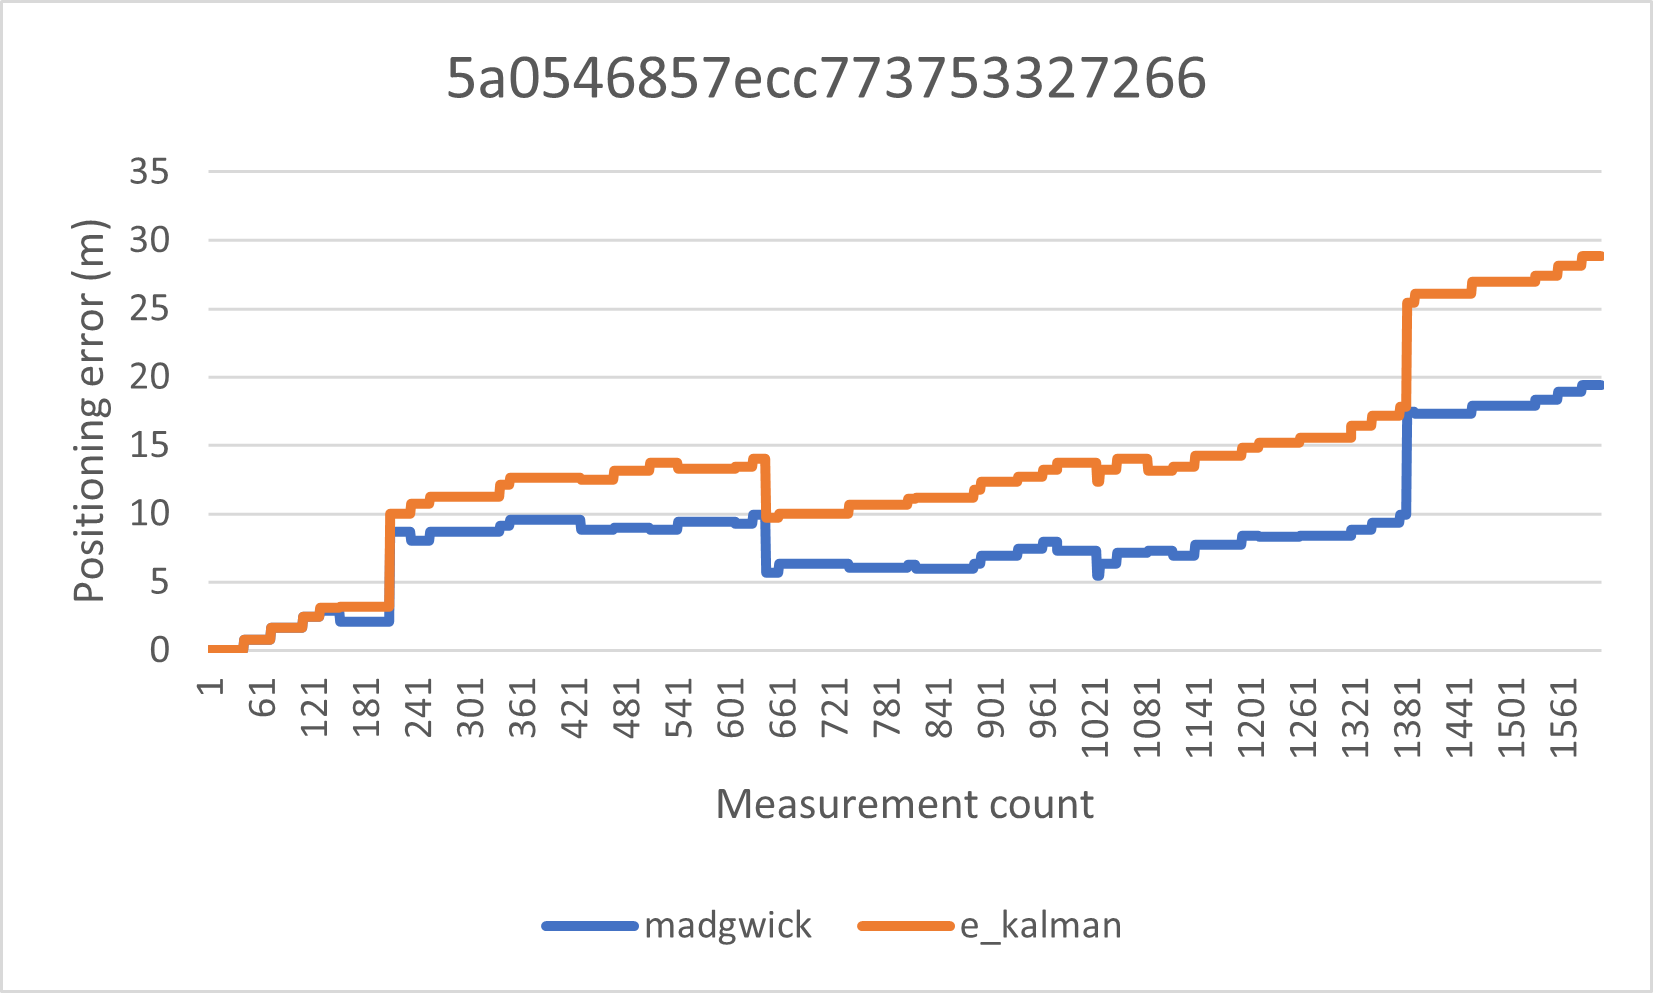
\includegraphics{Images/Experiments/pdr/pdr1.png}}
  \hfill
  \subfigure[]{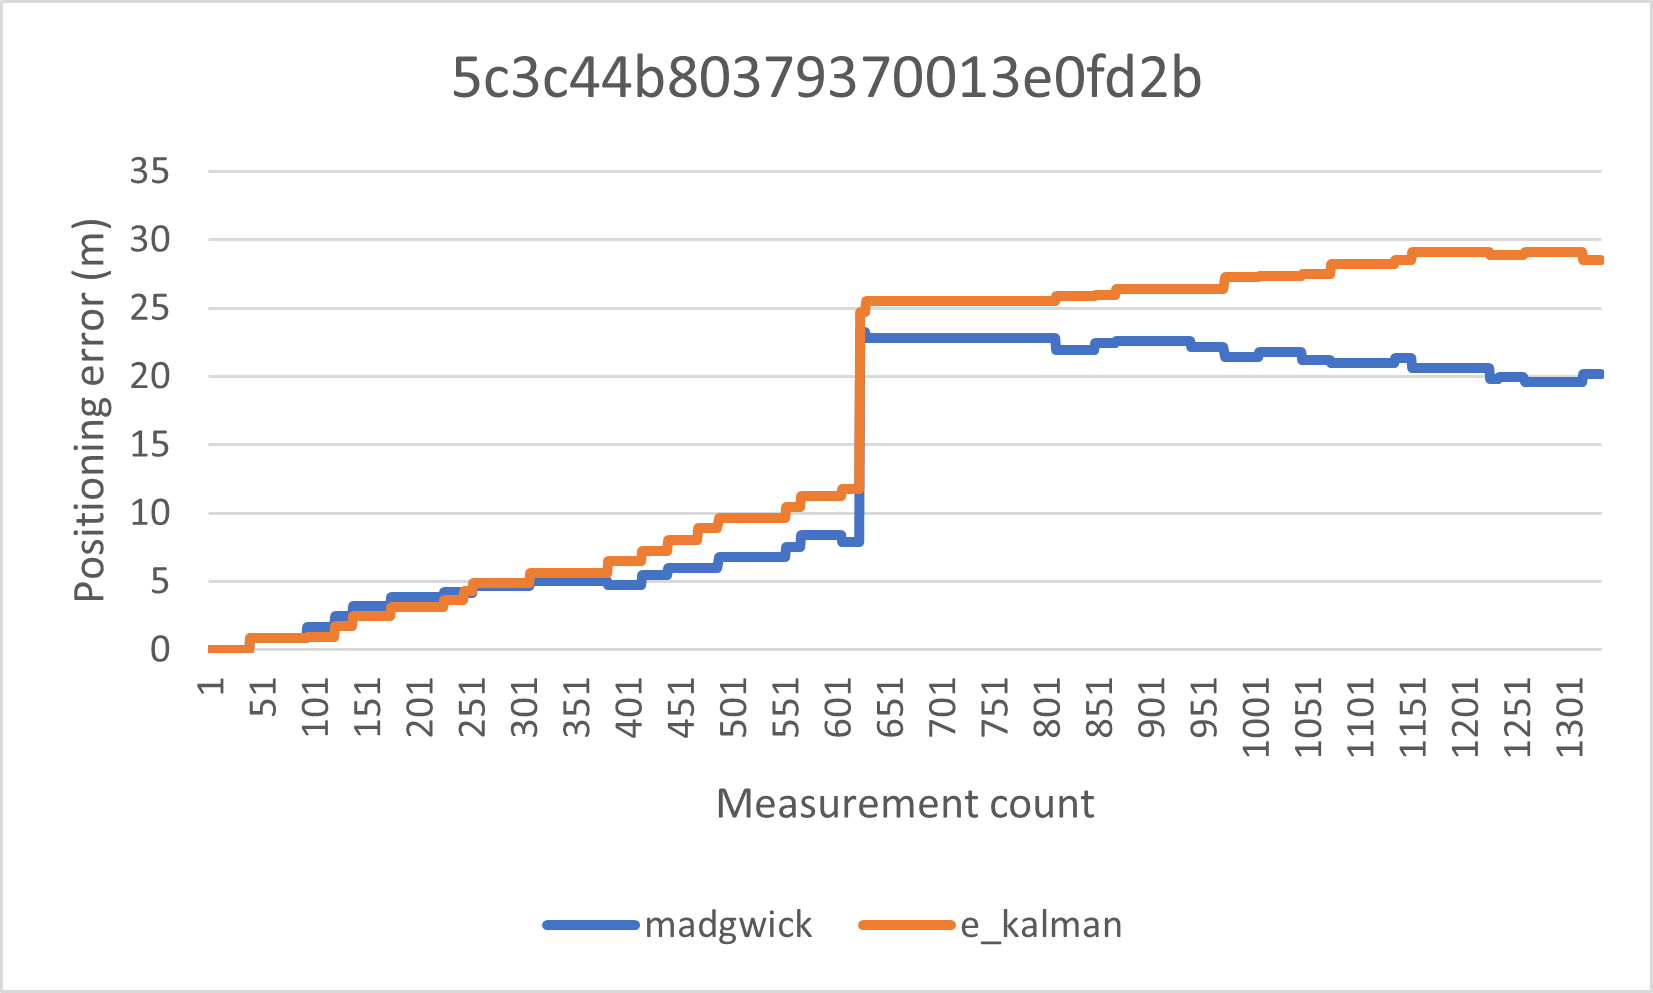
\includegraphics{Images/Experiments/pdr/pdr2.png}}
  \hfill
  \subfigure[]{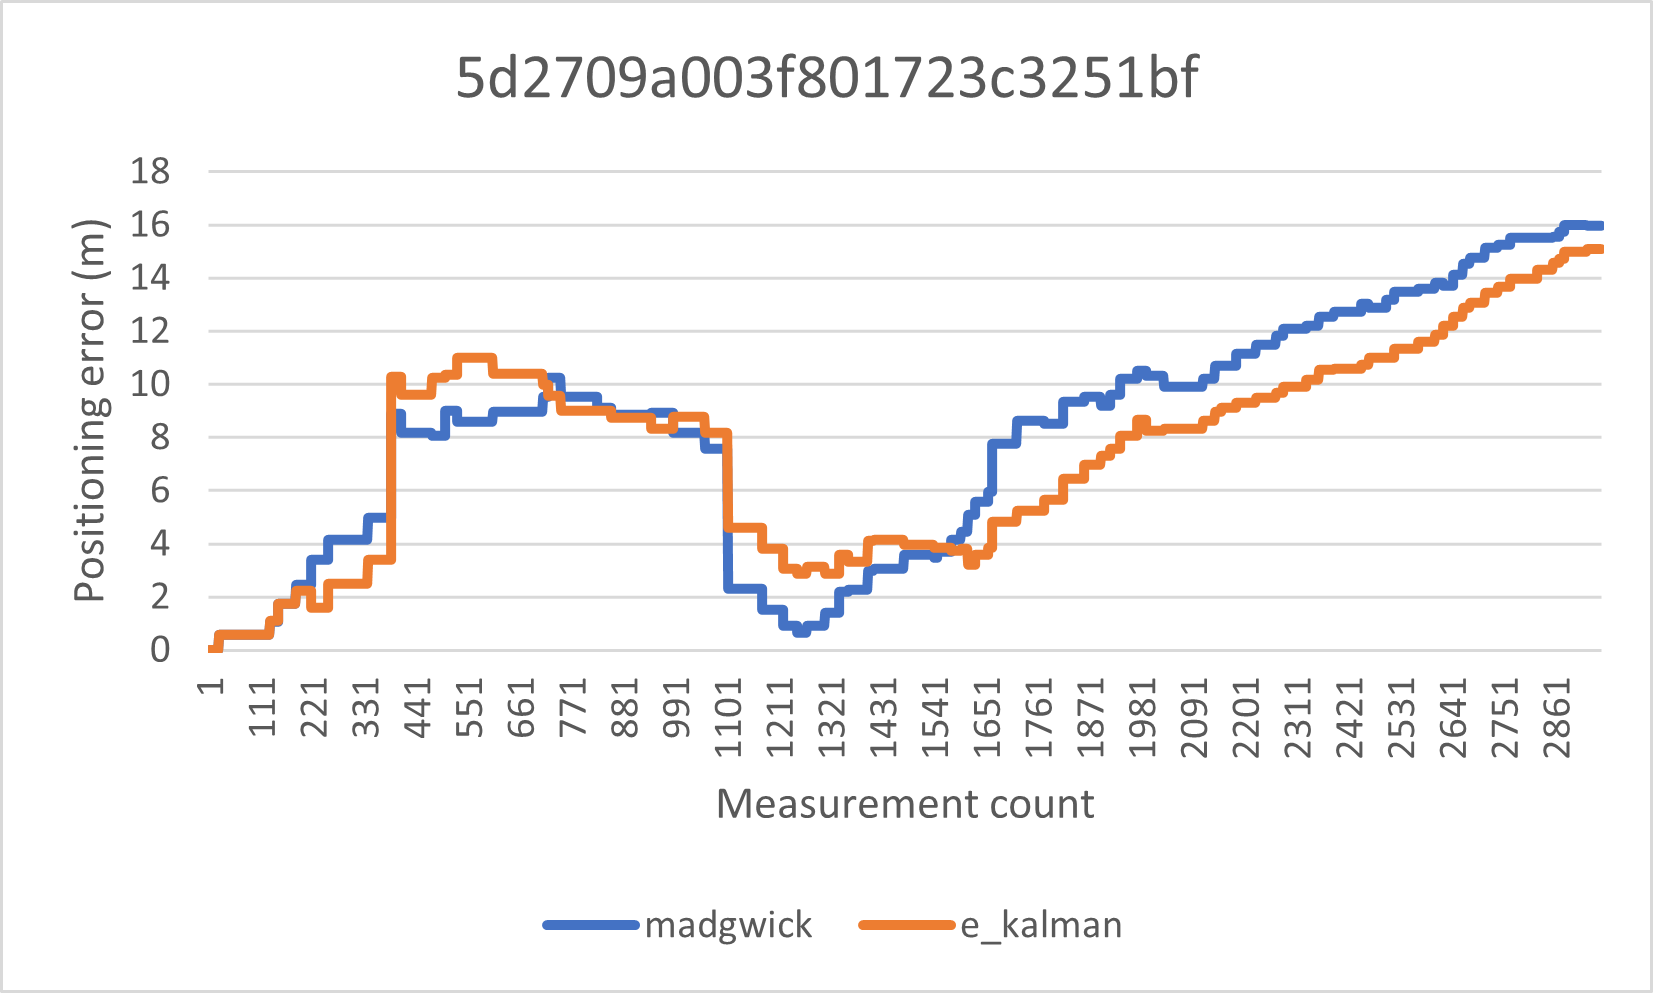
\includegraphics{Images/Experiments/pdr/pdr3.png}}
  \hfill
  \subfigure[]{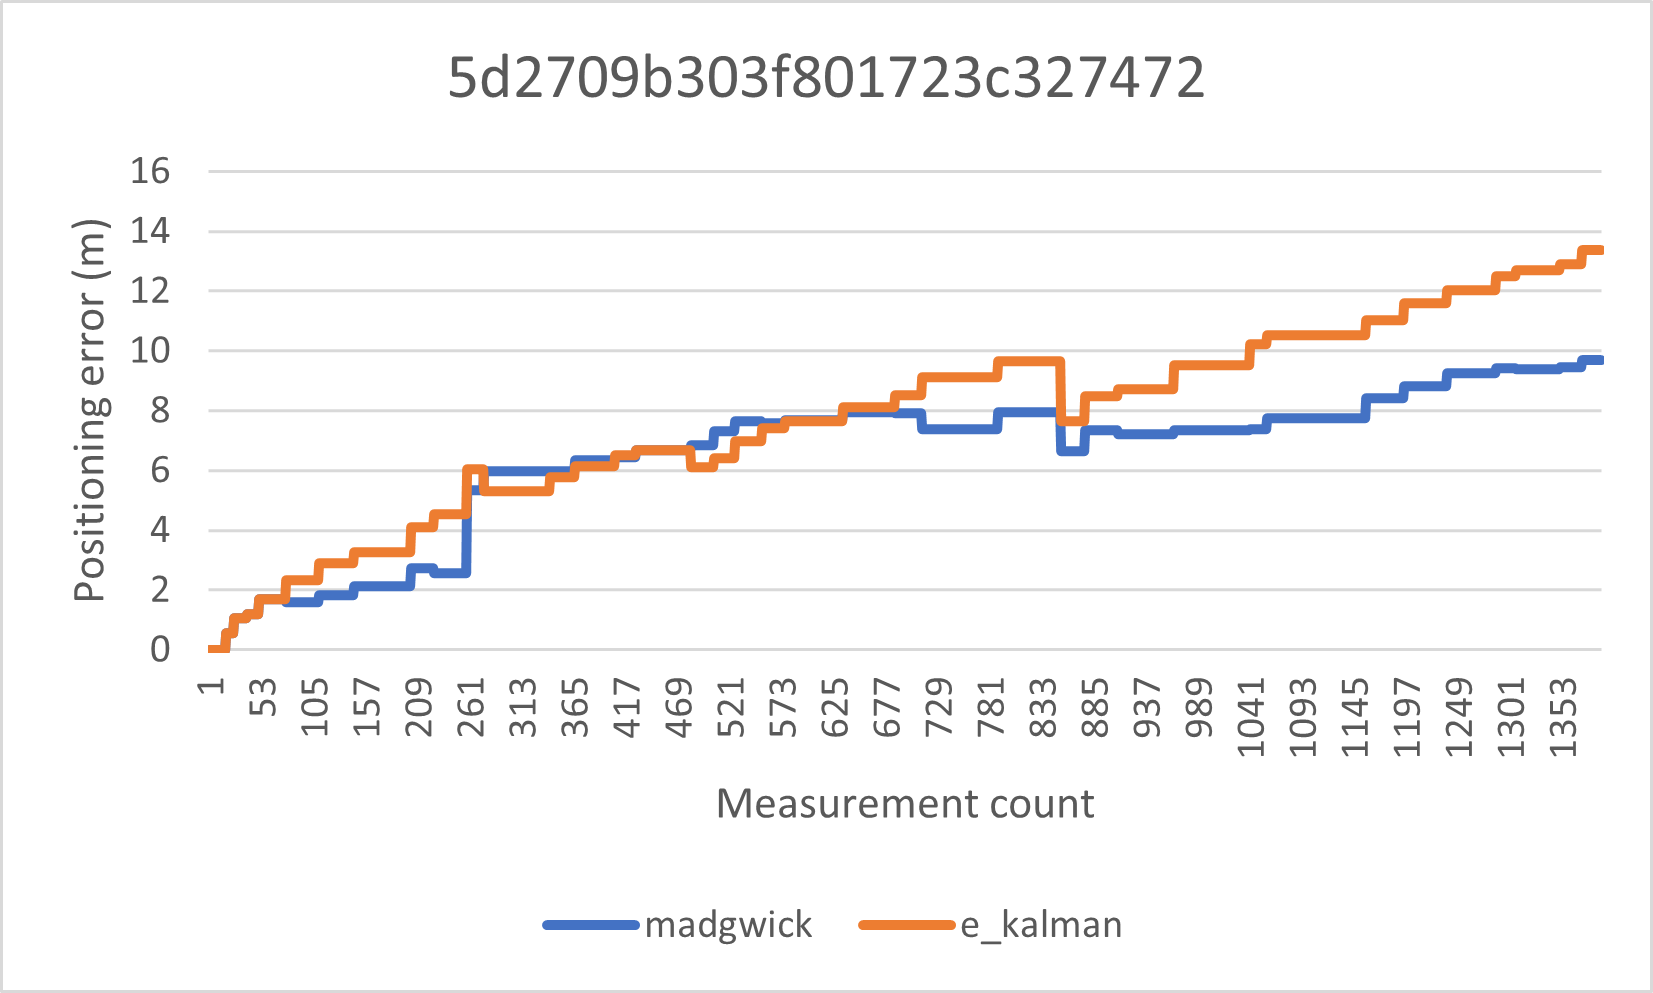
\includegraphics{Images/Experiments/pdr/pdr4.png}}
  \hfill
  \subfigure[]{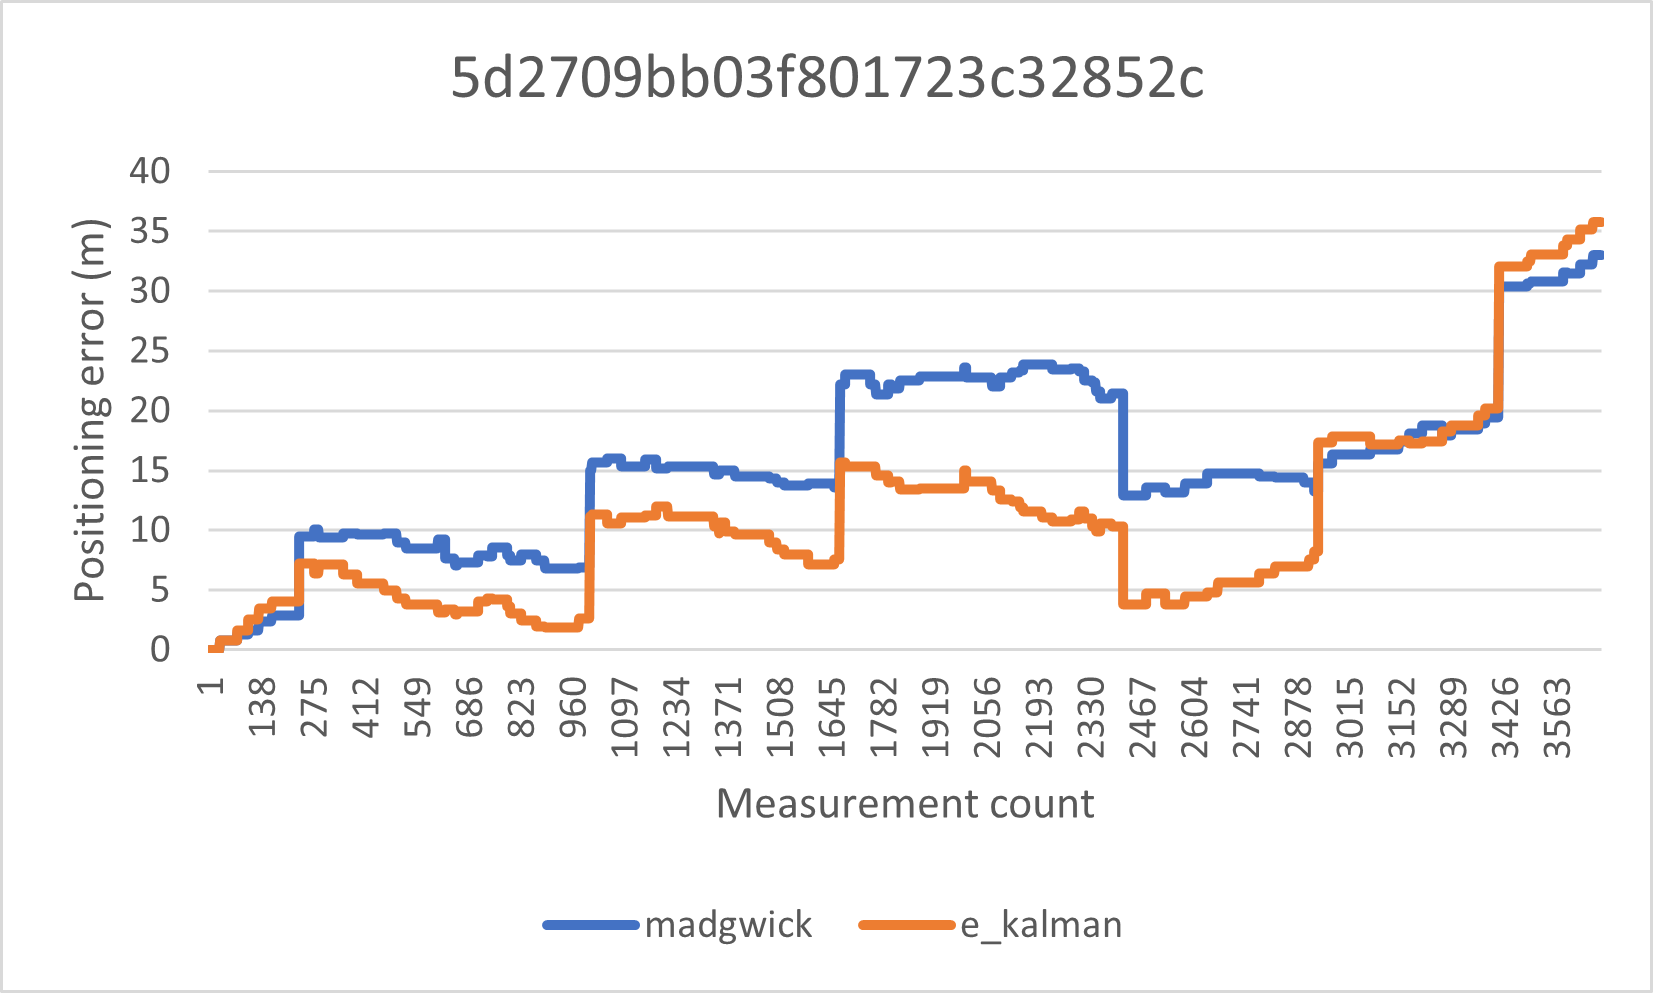
\includegraphics{Images/Experiments/pdr/pdr5.png}}
  \hfill  
  \subfigure[]{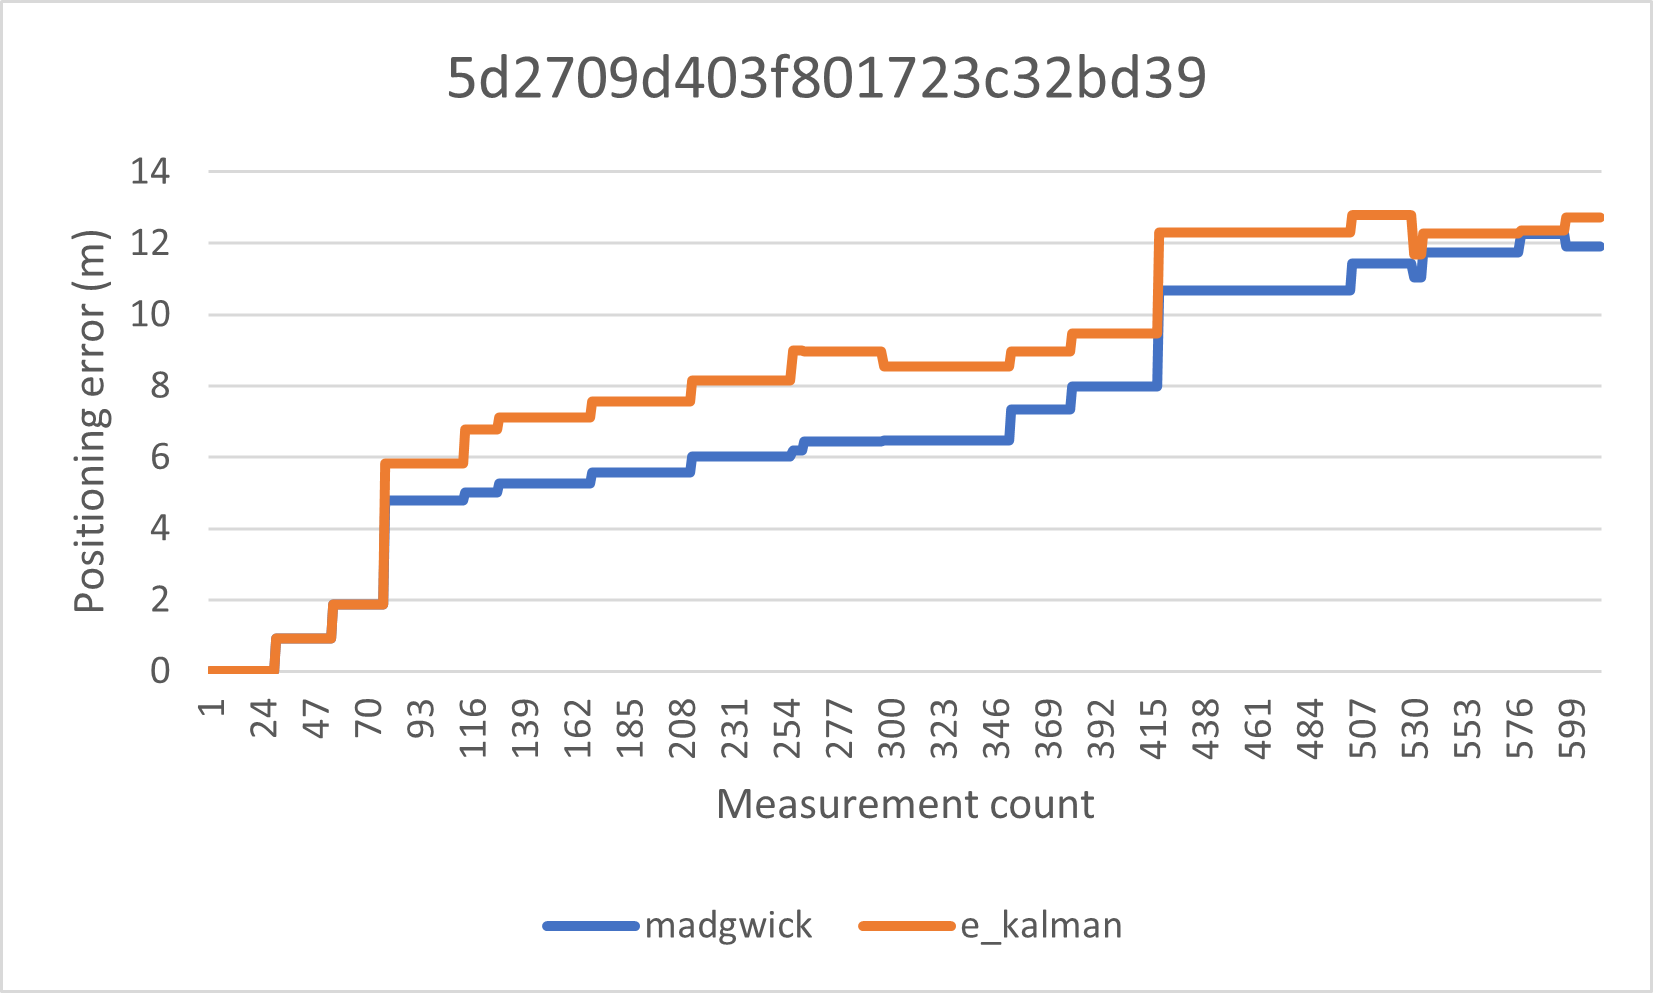
\includegraphics{Images/Experiments/pdr/pdr6.png}}
  \hfill
  \caption{\gls{pdr} performance using Madgwick Filter and Extended Kalman Filter for heading estimation.}
\end{figure}

\begin{figure}
\ContinuedFloat
\centering
\SetFigLayout{3}{2}  
  \subfigure[]{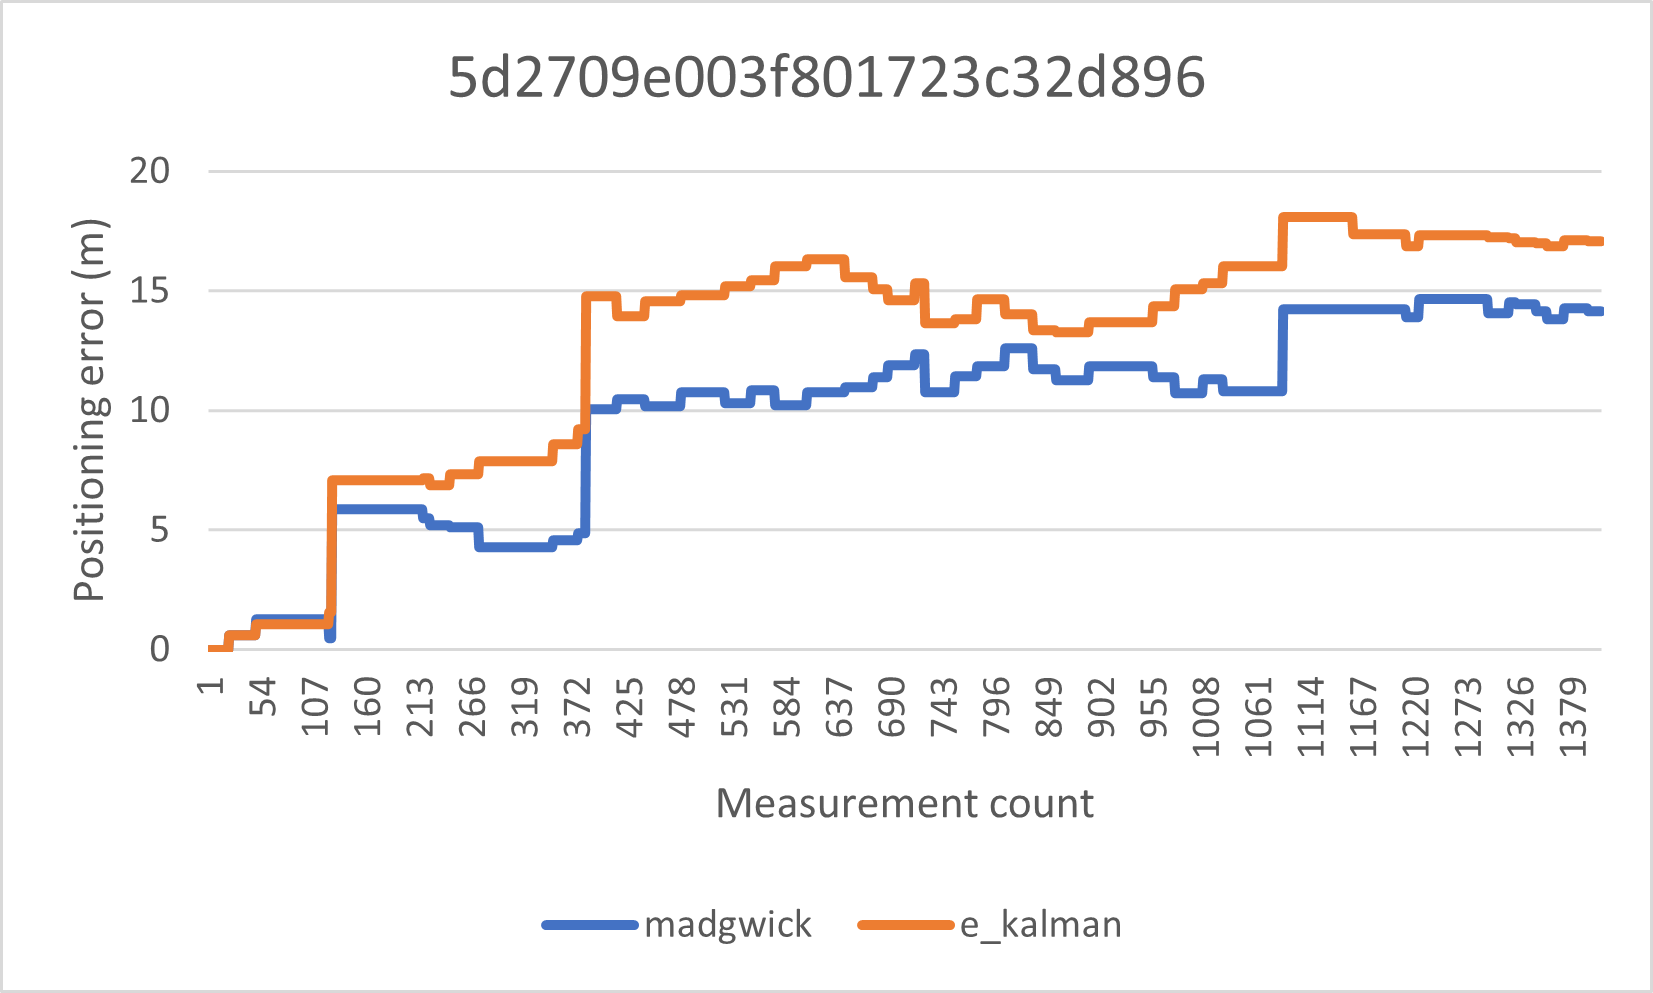
\includegraphics{Images/Experiments/pdr/pdr7.png}}
  \hfill
  \subfigure[]{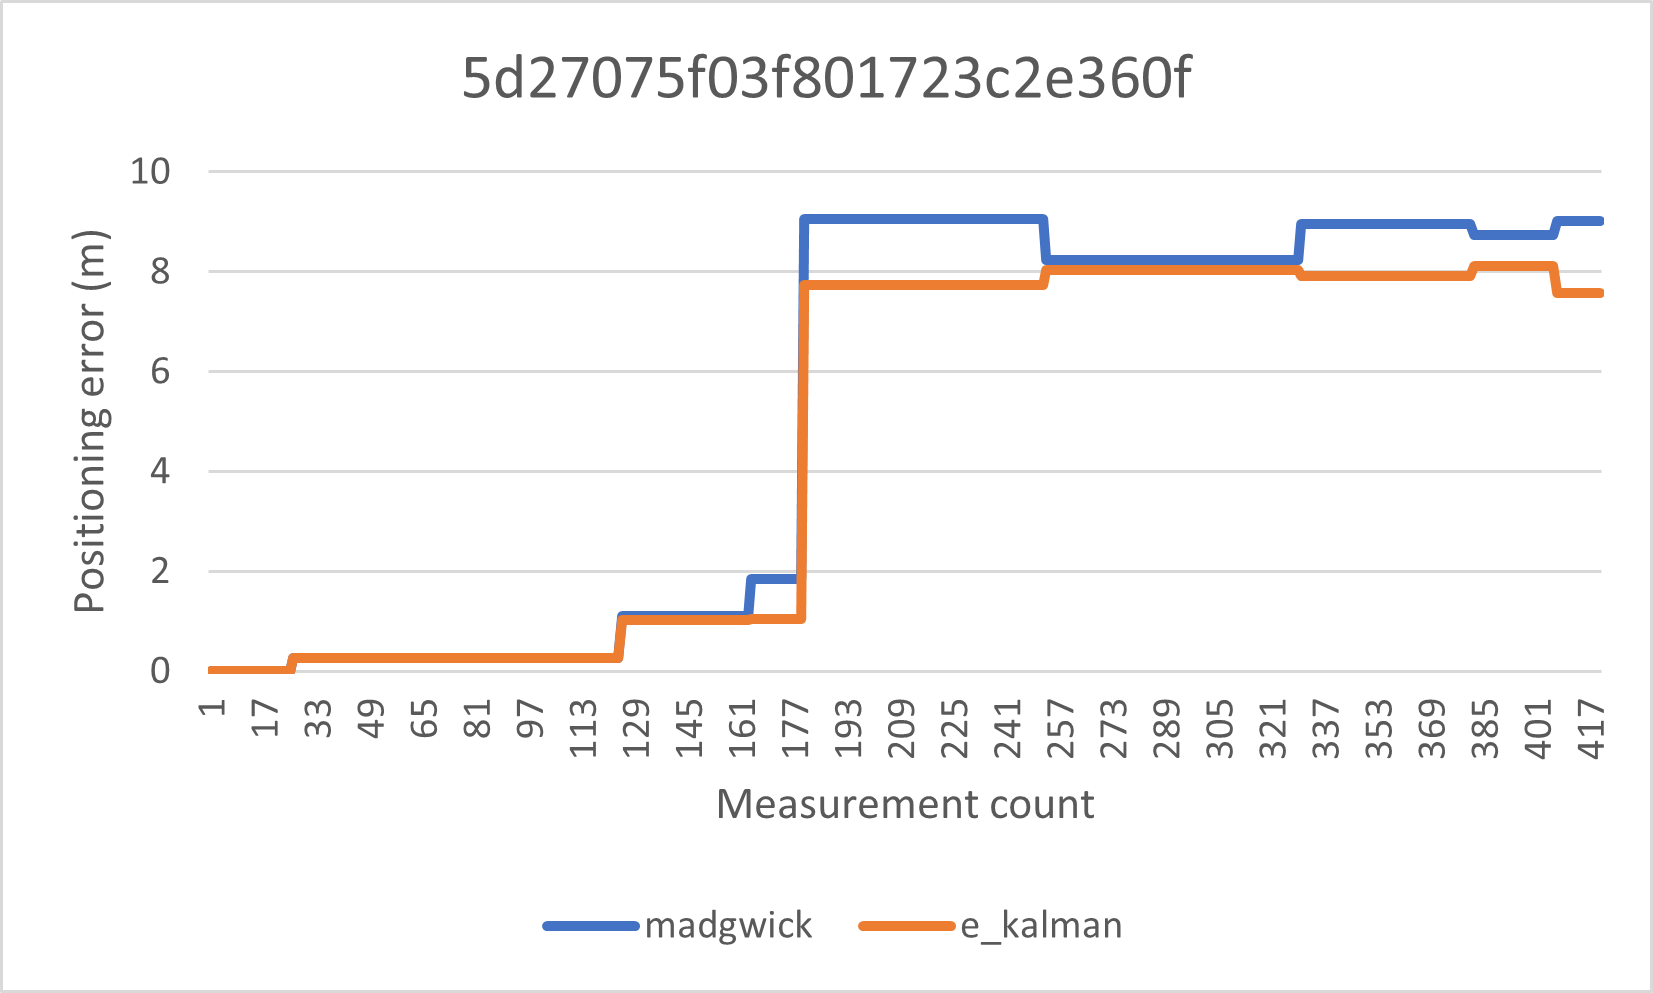
\includegraphics{Images/Experiments/pdr/pdr8.png}}
  \hfill
  \subfigure[]{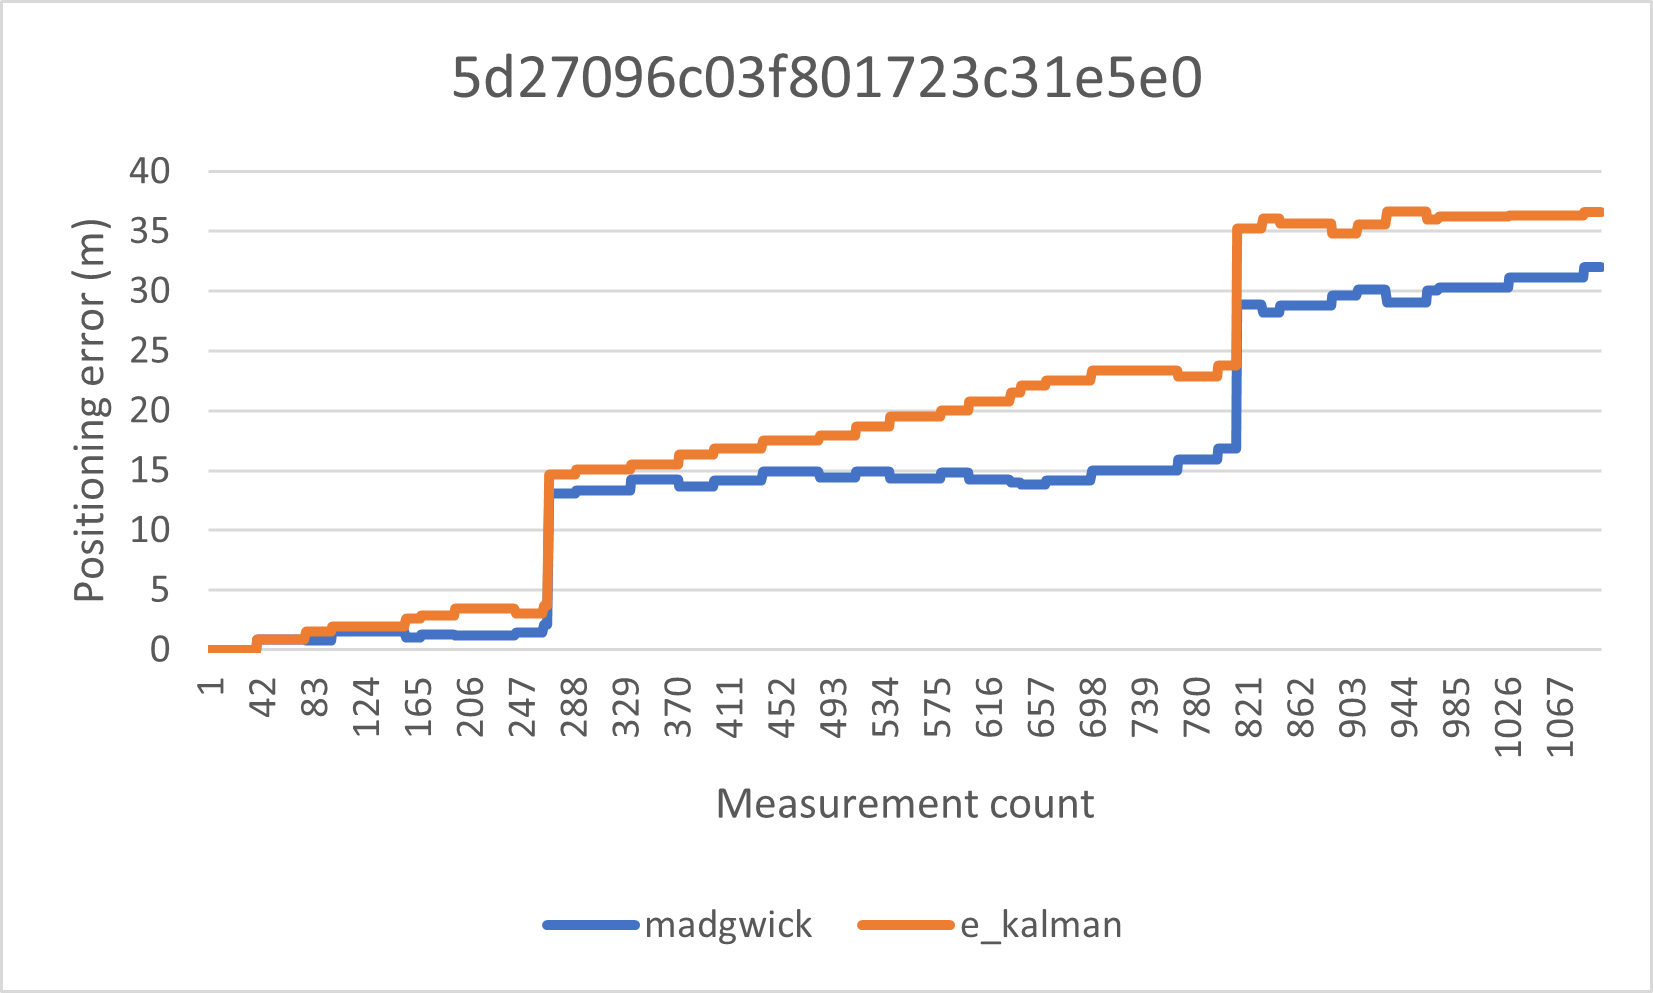
\includegraphics{Images/Experiments/pdr/pdr9.png}}
  \hfill
  \subfigure[]{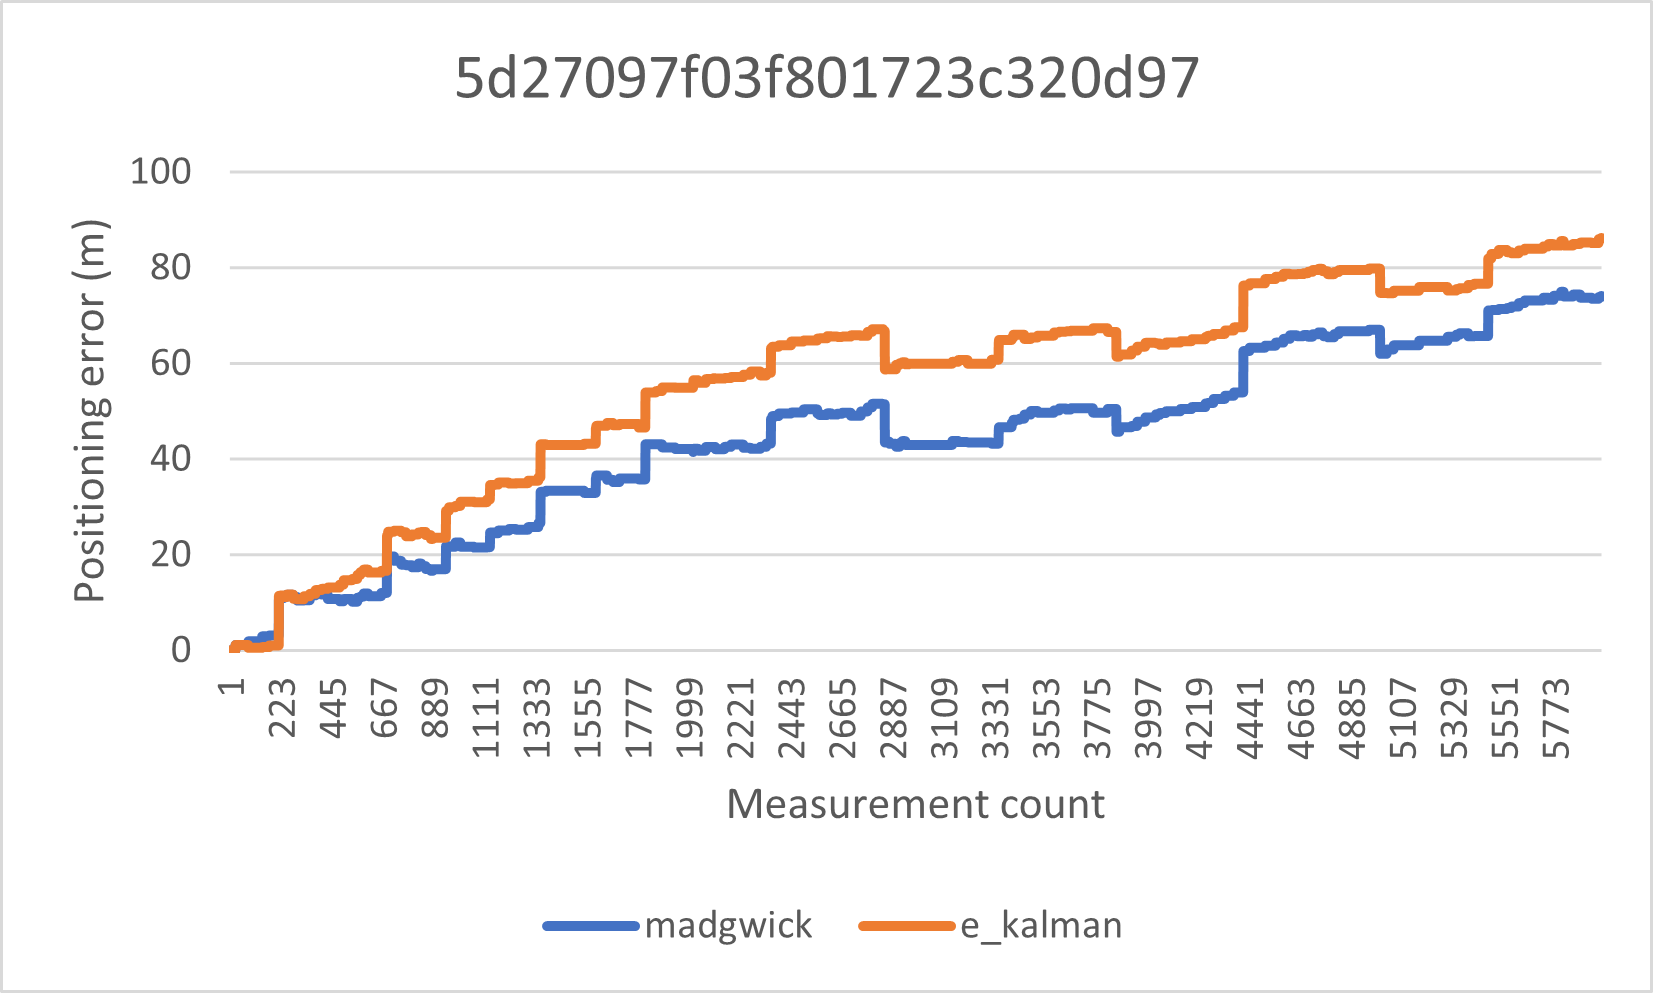
\includegraphics{Images/Experiments/pdr/pdr10.png}}
  \hfill
  \subfigure[]{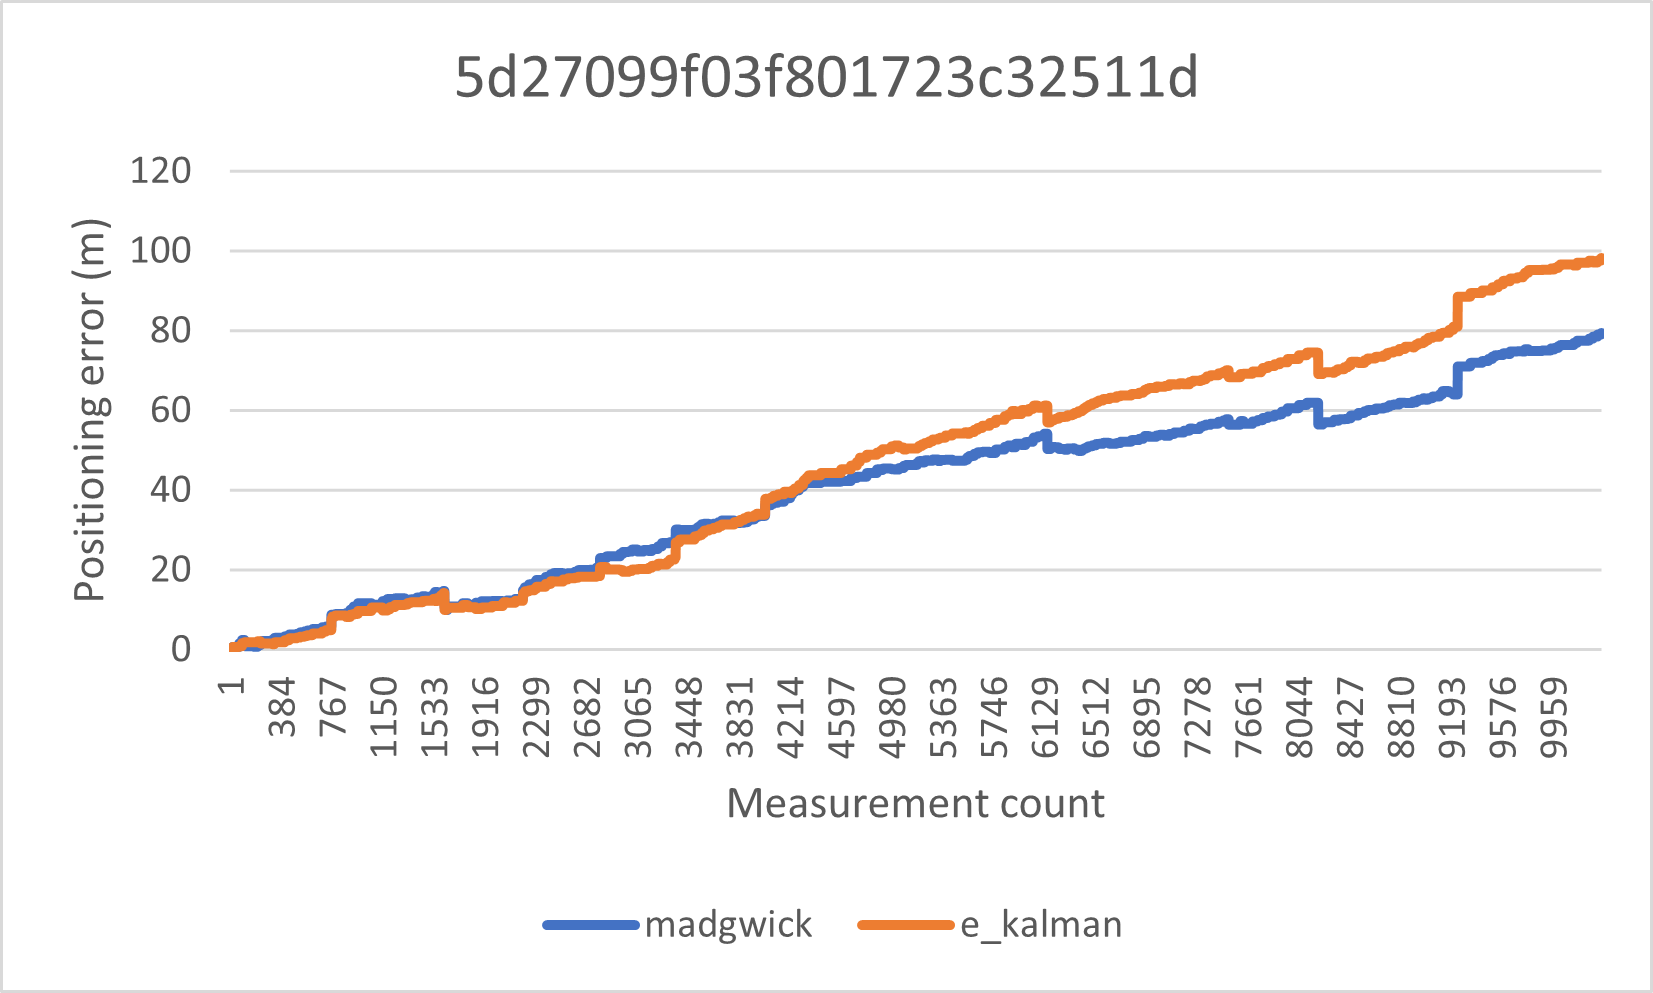
\includegraphics{Images/Experiments/pdr/pdr11.png}}
  \hfill
  \subfigure[]{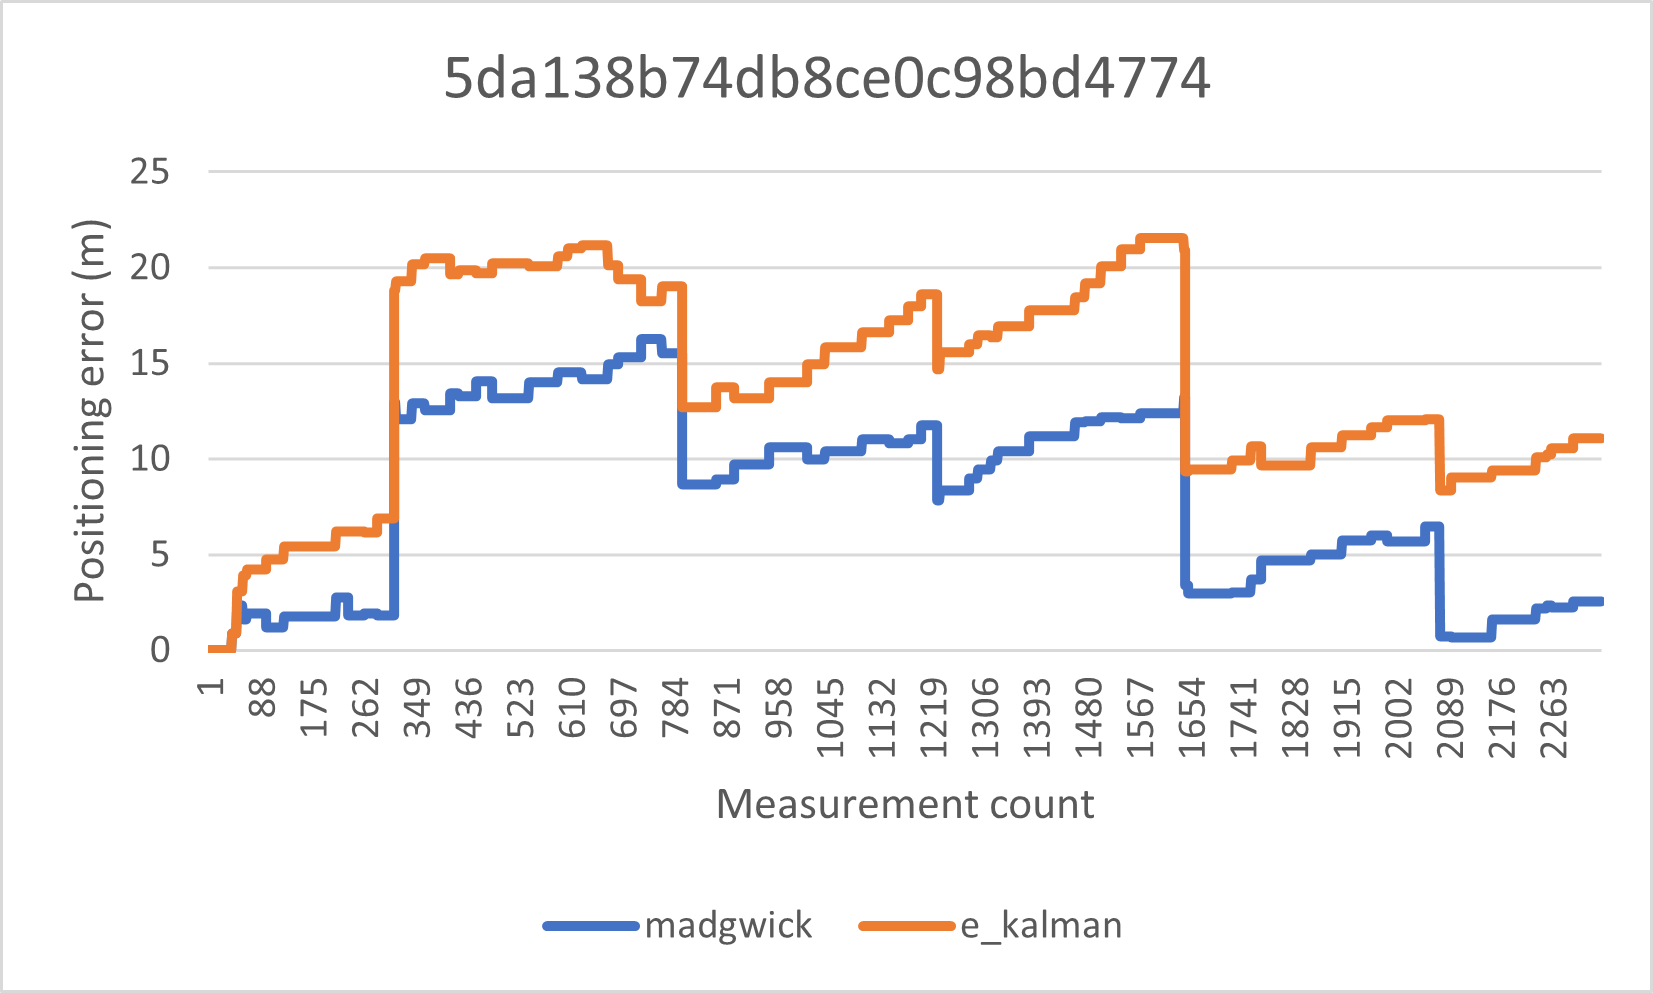
\includegraphics{Images/Experiments/pdr/pdr12.png}}
  \hfill
\caption{\gls{pdr} performance using Madgwick Filter and Extended Kalman Filter for heading estimation.}
\end{figure}

  \begin{figure}
\ContinuedFloat
\centering
\SetFigLayout{3}{2}  
  \subfigure[]{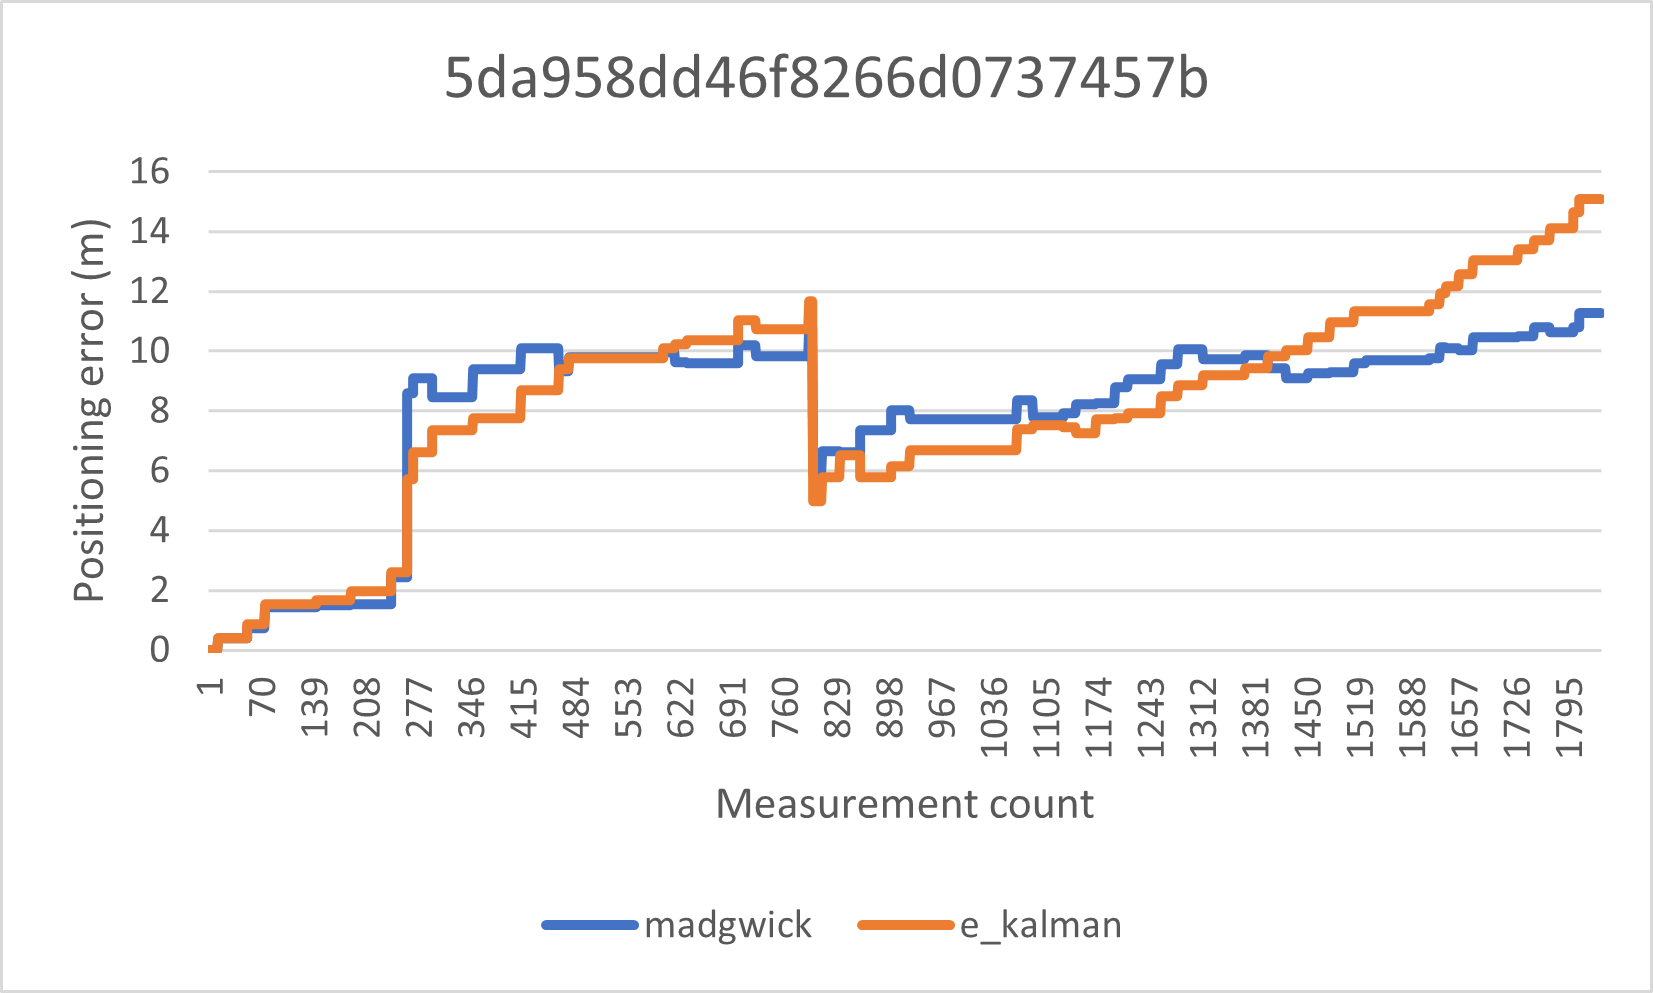
\includegraphics{Images/Experiments/pdr/pdr13.png}}
  \hfill
  \subfigure[]{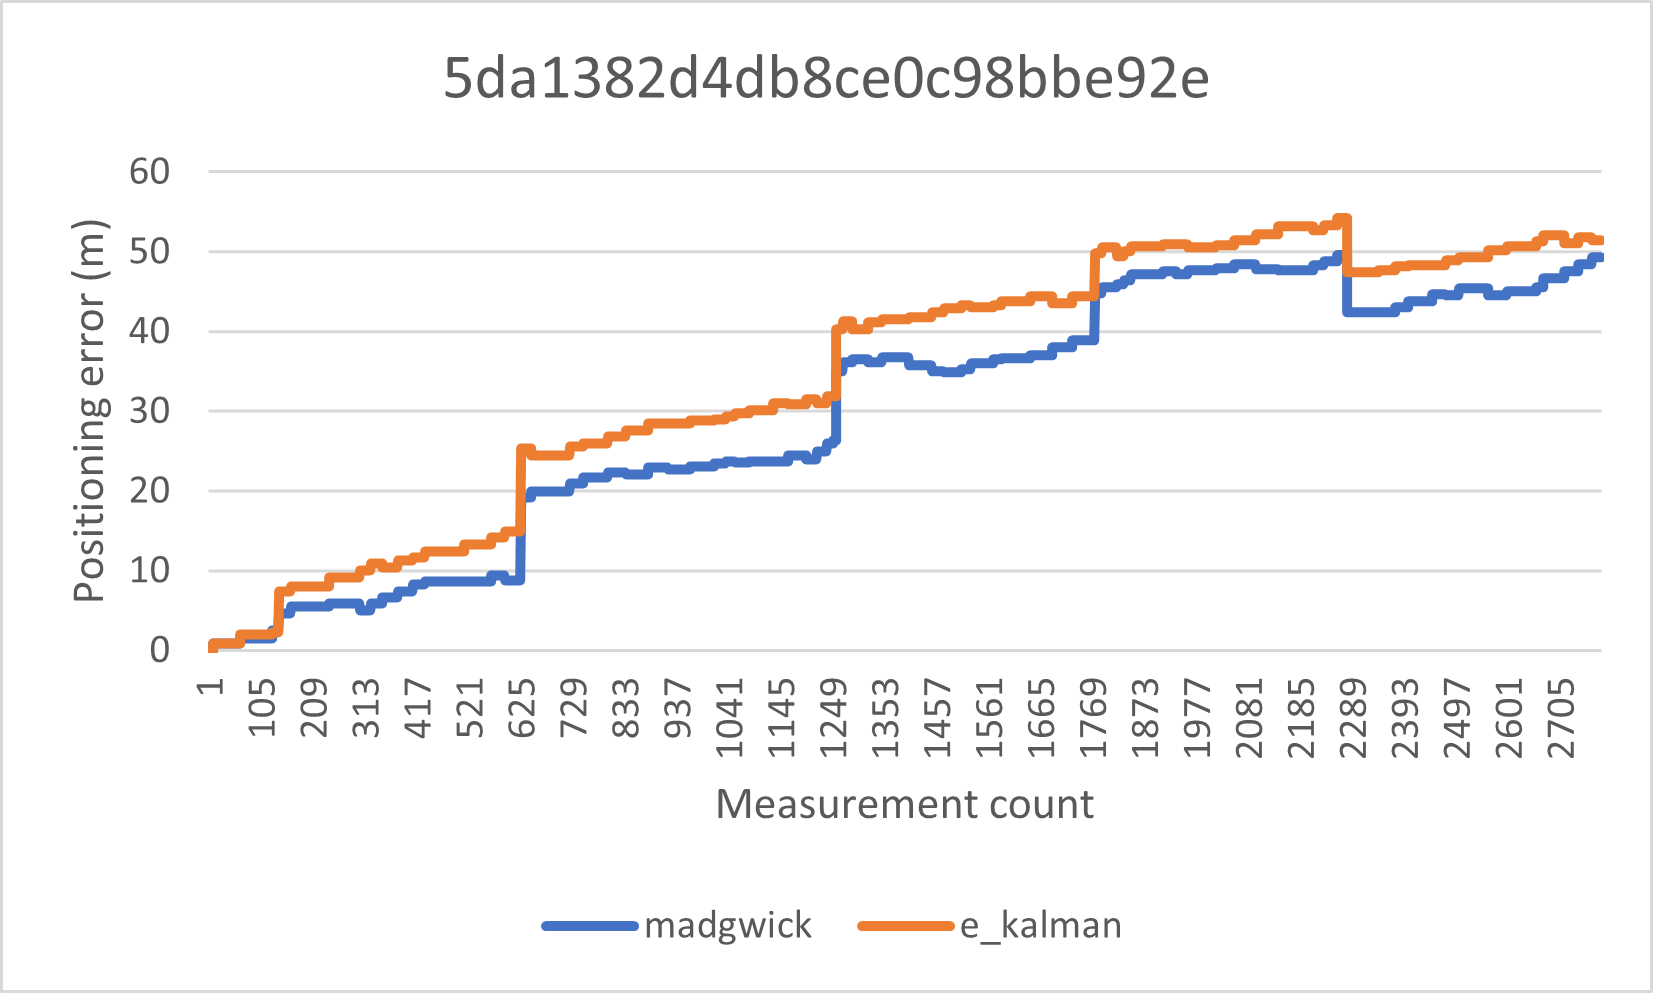
\includegraphics{Images/Experiments/pdr/pdr14.png}}
  \hfill
  \subfigure[]{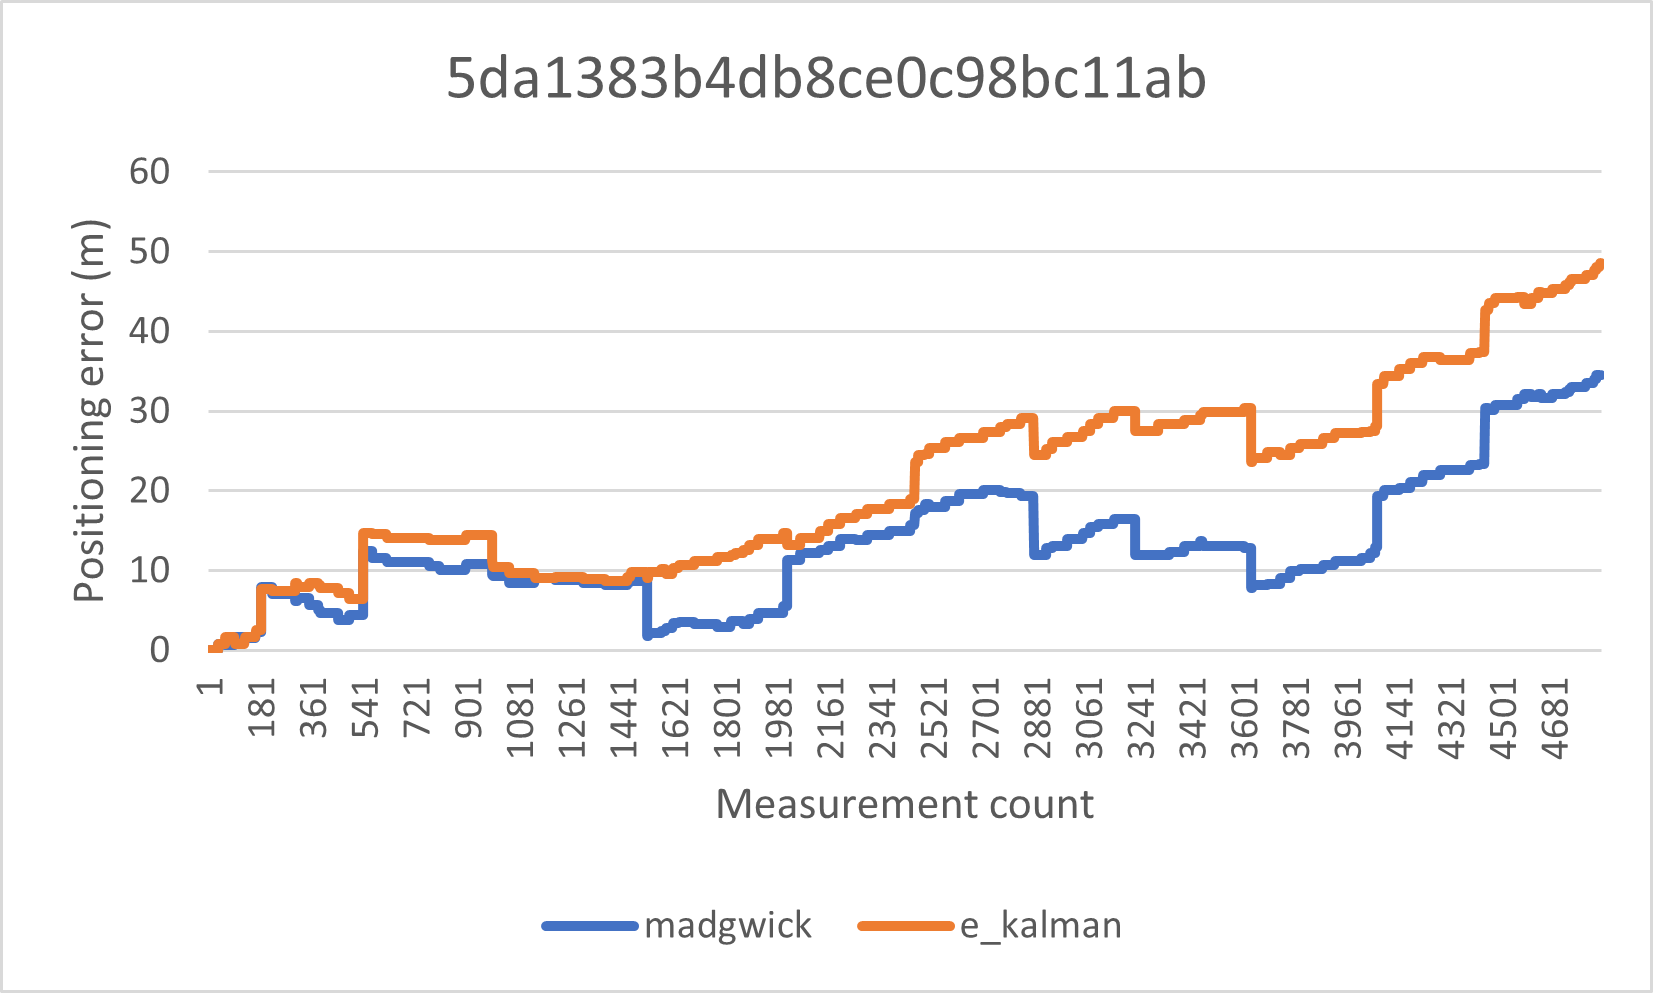
\includegraphics{Images/Experiments/pdr/pdr15.png}}
  \hfill
  \subfigure[]{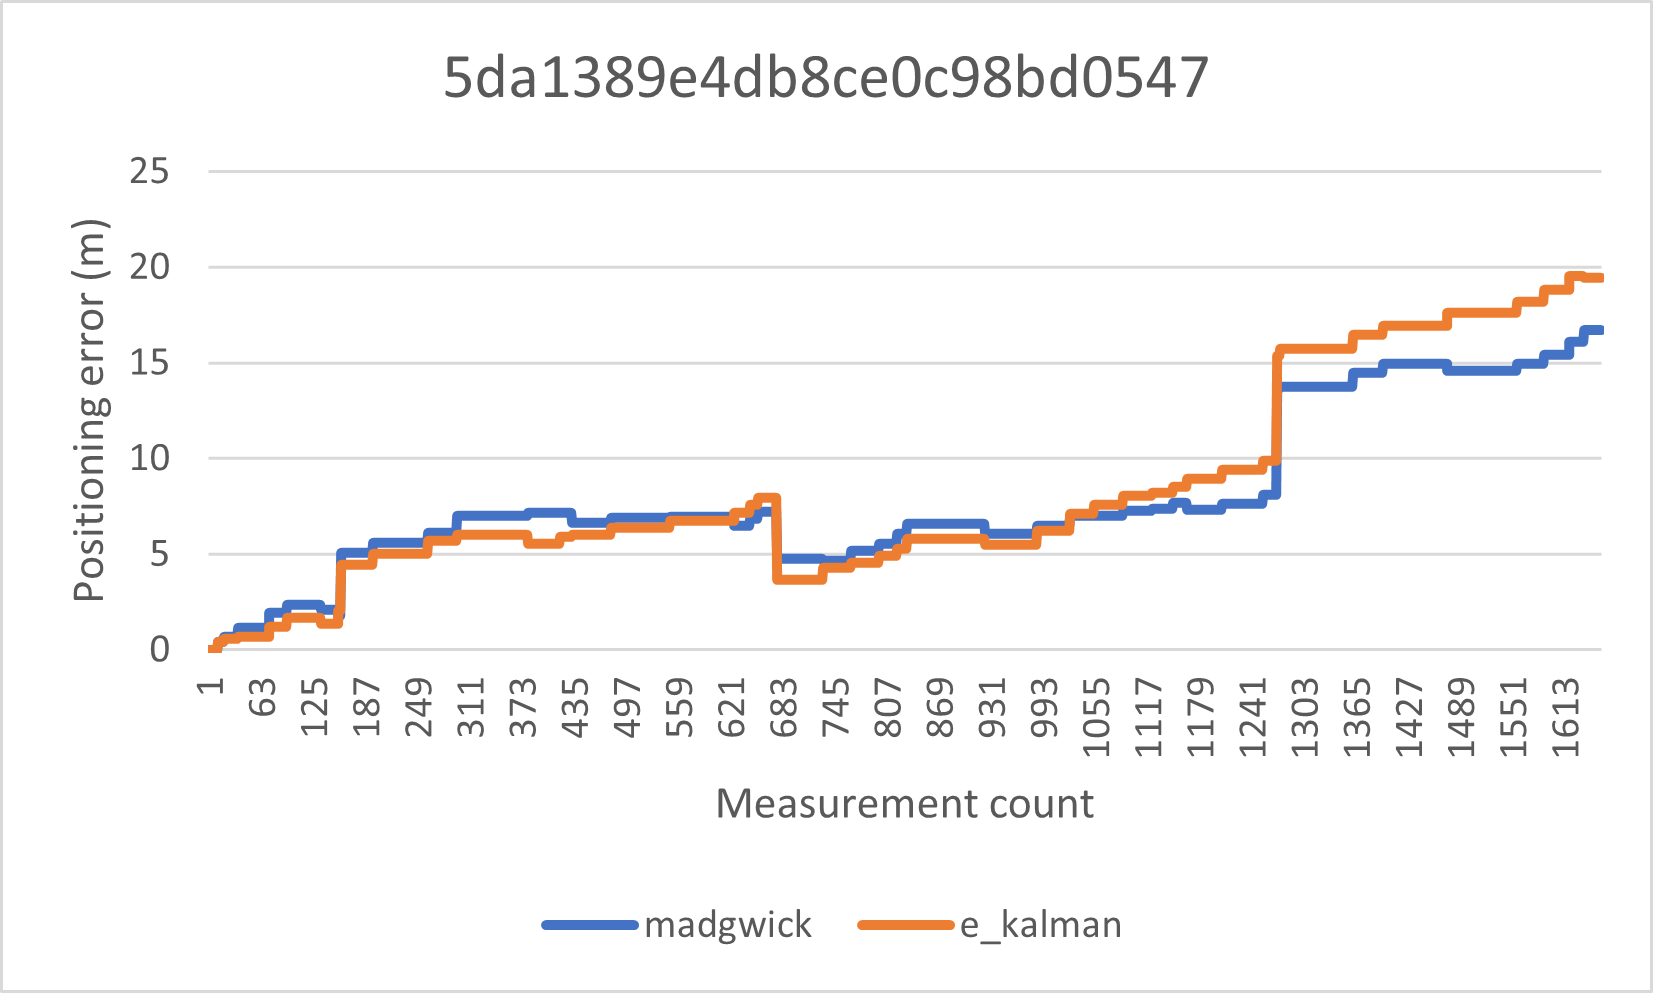
\includegraphics{Images/Experiments/pdr/pdr16.png}}
  \hfill
  \subfigure[]{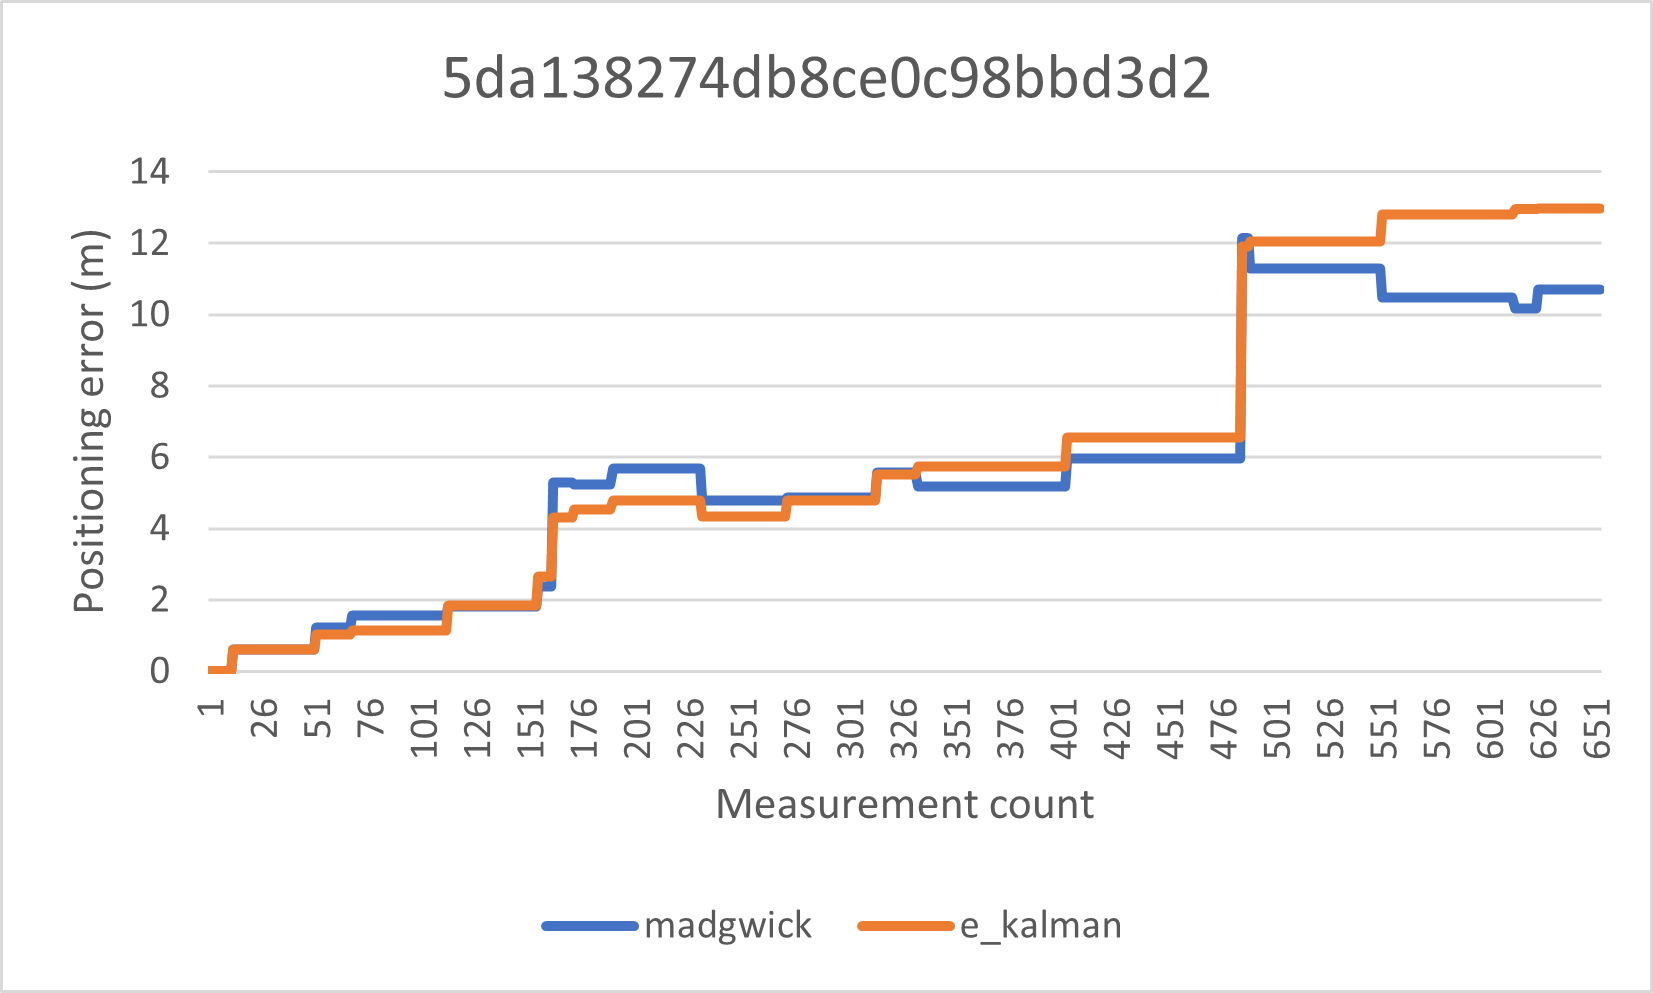
\includegraphics{Images/Experiments/pdr/pdr17.png}}
  \hfill
  \subfigure[]{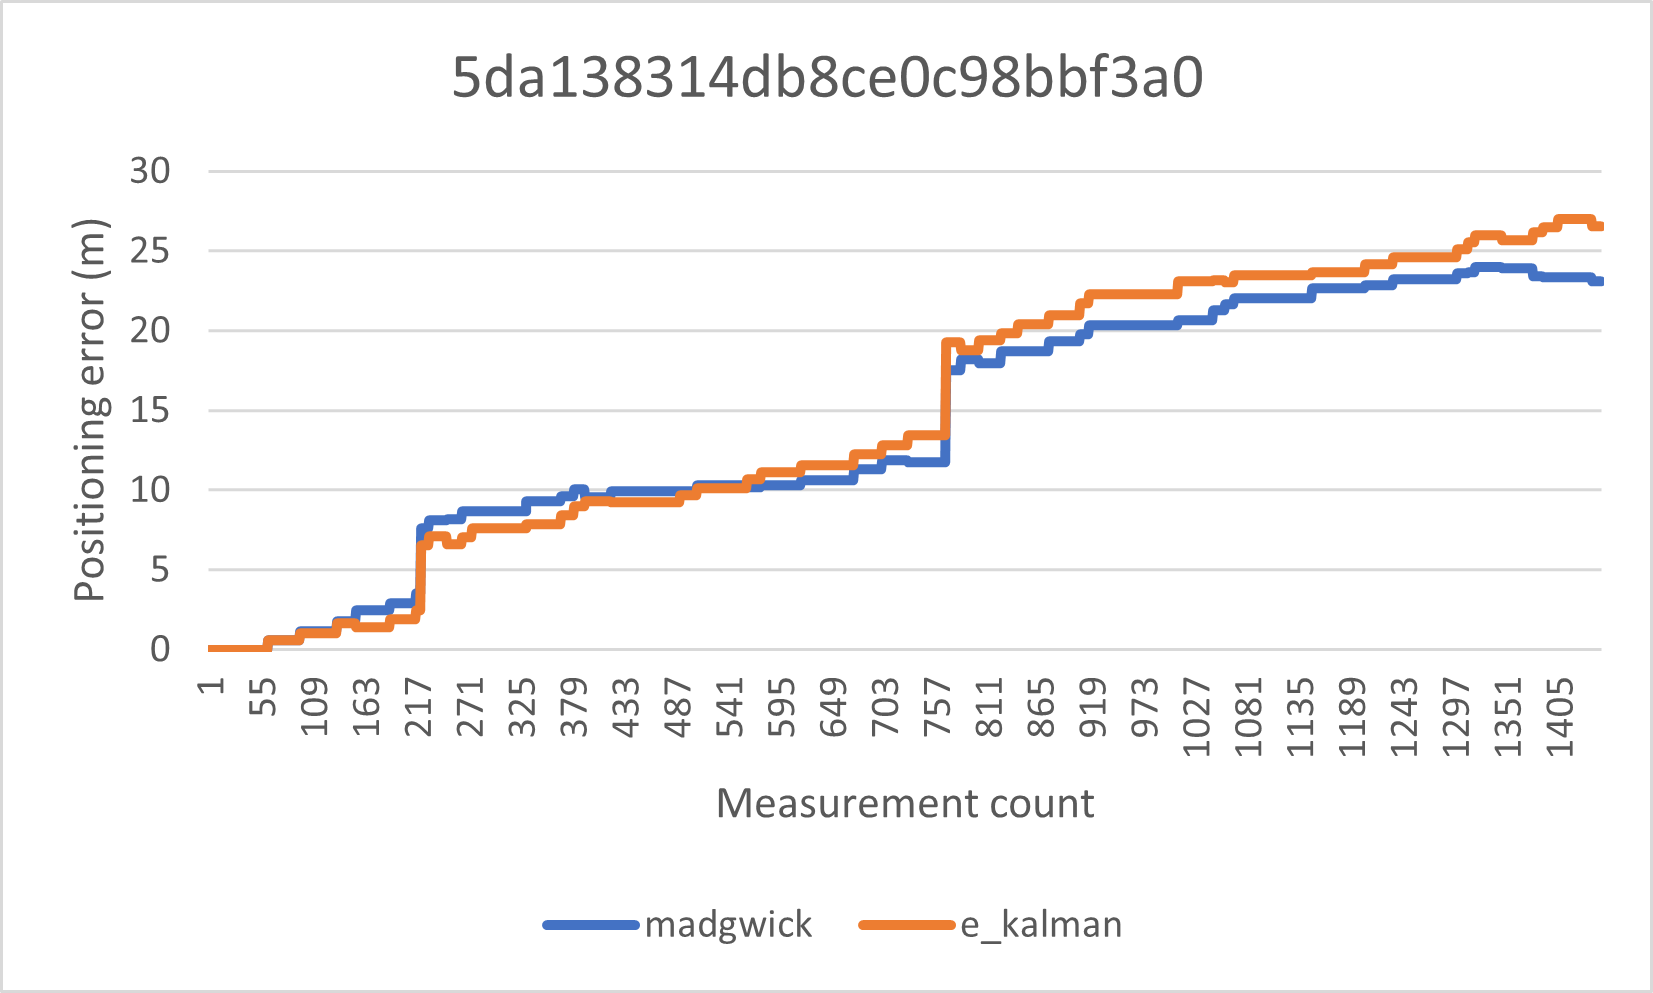
\includegraphics{Images/Experiments/pdr/pdr18.png}}
  \hfill
\caption{\gls{pdr} performance using Madgwick Filter and Extended Kalman Filter for heading estimation.}
\end{figure}

  \begin{figure}
\ContinuedFloat
\centering
\SetFigLayout{3}{2}  
  \subfigure[]{\includegraphics{Images/Experiments/pdr/pdr19.png}}
  \hfill
  \subfigure[]{\includegraphics{Images/Experiments/pdr/pdr20.png}}
  \hfill
  \subfigure[]{\includegraphics{Images/Experiments/pdr/pdr21.png}}
  \hfill
  \subfigure[]{\includegraphics{Images/Experiments/pdr/pdr22.png}}
  \hfill
  \subfigure[]{\includegraphics{Images/Experiments/pdr/pdr23.png}}
  \hfill
  \subfigure[]{\includegraphics{Images/Experiments/pdr/pdr24.png}}
  \hfill
\caption{\gls{pdr} performance using Madgwick Filter and Extended Kalman Filter for heading estimation.}
\end{figure}

%\markdownInput{offline.md}

%\part{Appendices}
%\appendixpageoff
%\begin{appendices}

%\end{appendices}
\end{document}